%%%%%%%% ICML 2025 EXAMPLE LATEX SUBMISSION FILE %%%%%%%%%%%%%%%%%

\documentclass{article}

% Recommended, but optional, packages for figures and better typesetting:
\usepackage{microtype}
\usepackage{graphicx}
\usepackage{subfigure}
\usepackage{booktabs} % for professional tables
\usepackage{longtable}
\usepackage{arydshln}
\usepackage{changepage} % provides adjustwidth



\usepackage{tikz}              % TikZ/PGF base
\usetikzlibrary{arrows.meta}   % modern arrow tips
\usetikzlibrary{positioning}   % for node distance etc.
\usetikzlibrary{calc}          % for coordinate math

\usetikzlibrary{arrows.meta,positioning,fit,calc}


\usepackage{amsmath, amssymb, bm}

% hyperref makes hyperlinks in the resulting PDF.
% If your build breaks (sometimes temporarily if a hyperlink spans a page)
% please comment out the following usepackage line and replace
% \usepackage{icml2025} with \usepackage[nohyperref]{icml2025} above.
\usepackage{hyperref}

%\usepackage{algorithm}
\usepackage{algpseudocode}

% Attempt to make hyperref and algorithmic work together better:
%\newcommand{\theHalgorithm}{\arabic{algorithm}}

% Use the following line for the initial blind version submitted for review:
% \usepackage{icml2025}

% If accepted, instead use the following line for the camera-ready submission:
\usepackage[preprint]{icml2026}
%\usepackage{icml2025}

% For theorems and such
\usepackage{amsmath}
\usepackage{amssymb}
\usepackage{mathtools}
\usepackage{amsthm}
\usepackage{arydshln}

% if you use cleveref..
\usepackage[capitalize,noabbrev]{cleveref}

\input{math_commands}


%%%%%%%%%%%%%%%%%%%%%%%%%%%%%%%%
% THEOREMS
%%%%%%%%%%%%%%%%%%%%%%%%%%%%%%%%
\theoremstyle{plain}
\newtheorem{theorem}{Theorem}[section]
\newtheorem{proposition}[theorem]{Proposition}
\newtheorem{lemma}[theorem]{Lemma}
\newtheorem{corollary}[theorem]{Corollary}
\theoremstyle{definition}
\newtheorem{definition}[theorem]{Definition}
\newtheorem{assumption}[theorem]{Assumption}
\theoremstyle{remark}
\newtheorem{remark}[theorem]{Remark}
\renewcommand{\appendixautorefname}{App.}

% Todonotes is useful during development; simply uncomment the next line
%    and comment out the line below the next line to turn off comments
%\usepackage[disable,textsize=tiny]{todonotes}
\usepackage[textsize=tiny]{todonotes}
\usepackage{xcolor}

\definecolor{mygray}{gray}{0.9}


% The \icmltitle you define below is probably too long as a header.
% Therefore, a short form for the running title is supplied here:
\icmltitlerunning{Leech Lattice Vector Quantization}

\begin{document}

\twocolumn[
%\icmltitle{A Leech Lattice Vector Quantizer}
%\icmltitle{Quantizing LLMs using the Leech Lattice}
%\icmltitle{Quantizing LLMs using Leech Spherical Codes}
%\icmltitle{LLVQ: Leech Lattice Vector Quantization}
%\icmltitle{LLVQ: Leech Lattice Vector Quantization for efficient LLM Compression}
%\icmltitle{Quantizing LLMs using Leech Lattice Spherical Codes}
% \icmltitle{A Leech Lattice Vector Quantizer for LLM Model Efficiency}
\icmltitle{Leech Lattice Vector Quantization for Efficient LLM Compression}
%\icmltitle{A Leech Lattice Vector Quantizer for \\ 2 bit Post-Training LLM Quantization}

% It is OKAY to include author information, even for blind
% submissions: the style file will automatically remove it for you
% unless you've provided the [accepted] option to the icml2025
% package.

% List of affiliations: The first argument should be a (short)
% identifier you will use later to specify author affiliations
% Academic affiliations should list Department, University, City, Region, Country
% Industry affiliations should list Company, City, Region, Country

% You can specify symbols, otherwise they are numbered in order.
% Ideally, you should not use this facility. Affiliations will be numbered
% in order of appearance and this is the preferred way.
%\icmlsetsymbol{equal}{*}

\begin{icmlauthorlist}
\icmlauthor{Tycho F. A. van der Ouderaa}{qualcomm}
\icmlauthor{Mart van Baalen}{qualcomm}
\icmlauthor{Paul Whatmough}{qualcomm}
\icmlauthor{Markus Nagel}{qualcomm}
%\icmlauthor{}{sch}
%\icmlauthor{}{sch}
\end{icmlauthorlist}

\icmlaffiliation{qualcomm}{Qualcomm AI Research. Qualcomm AI Research is an initiative of Qualcomm Technologies, Inc}

% \icmlcorrespondingauthor{Tycho F. A. van der Ouderaa}{touderaa@qti.qualcomm.com}
\icmlcorrespondingauthor{}{\{touderaa,mart,pwhatmou,markusn\}@qti.qualcomm.com}

% You may provide any keywords that you
% find helpful for describing your paper; these are used to populate
% the "keywords" metadata in the PDF but will not be shown in the document
\icmlkeywords{Machine Learning, ICML}

\vskip 0.3in
]

% this must go after the closing bracket ] following \twocolumn[ ...

% This command actually creates the footnote in the first column
% listing the affiliations and the copyright notice.
% The command takes one argument, which is text to display at the start of the footnote.
% The \icmlEqualContribution command is standard text for equal contribution.
% Remove it (just {}) if you do not need this facility.

\printAffiliationsAndNotice{}  % leave blank if no need to mention equal contribution
% \printAffiliationsAndNotice{\icmlEqualContribution} % otherwise use the standard text.

% While recent work leveraged the E8 lattice (8 dimensions), t
\begin{abstract}
Scalar quantization of large language models (LLMs) is fundamentally limited by information-theoretic bounds. While vector quantization (VQ) overcomes these limits by encoding blocks of parameters jointly,  practical implementations must avoid the need for expensive lookup mechanisms or other explicit codebook storage. Lattice approaches address this through highly structured and dense packing.
This paper explores the Leech lattice, which, with its optimal sphere packing and kissing configurations at 24 dimensions, is the highest dimensional lattice known with such optimal properties. To make the Leech lattice usable for LLM quantization, we extend an existing search algorithm based on the extended Golay code construction, to i) support indexing, enabling conversion to and from bitstrings without materializing the codebook, ii) allow angular search over union of Leech lattice shells, iii) propose fully-parallelisable dequantization kernel. Together this yields a practical algorithm, namely \emph{Leech Lattice Vector Quantization} (LLVQ). LLVQ delivers state-of-the-art LLM quantization performance, outperforming recent methods such as Quip\#, QTIP, and PVQ. These results highlight the importance of high-dimensional lattices for scalable, theoretically grounded model compression.
\end{abstract}

\section{Introduction}
\label{introduction}

Quantization is a critical technique for compressing large language models (LLMs). Traditionally, this has been approached through scalar quantization, where individual weights are represented using fewer bits. While simple and widely adopted, classical results in rate–distortion theory (originating with Shannon) show that memoryless mappings are, in general, suboptimal: achieving the optimal distortion at a given rate typically requires coding over blocks rather than symbol-by-symbol mappings \citep{shannon1948mathematical,shannon1959coding}. Perhaps surprisingly, this even holds for completely independent and isotropically distributed sources, such as Gaussian vectors, where block coding strictly outperforms scalar methods in the rate-distortion trade-off \citep{gray2002quantization}. Consequently, scalar quantization is fundamentally limited when targeting aggressive compression without significant accuracy loss.

To overcome these limitations, vector quantization (VQ) \citep{gersho2012vector} encodes \emph{blocks} of weights jointly. Concretely, a $d$‑dimensional block represented by a $b$‑bit index selects one codeword from a set of size $2^{b}$, yielding an average rate of $b/d$ bits per weight. From a deep‑learning practitioner’s perspective, this is akin to assigning a dedicated \emph{dtype} to an entire block of weights rather than to each scalar entry: the block is stored as a single compact integer index instead of many independent scalars. A \emph{naive} realization of this idea is to materialize the codebook explicitly and perform nearest‑neighbor lookup among its $2^{b}$ high‑dimensional codewords. \emph{GPTVQ} \citep{van2024gptvq} demonstrates that such unstructured VQ can be applied to LLMs; however, the explicit‑table approach scales poorly with dimension $d$, because both storage and lookup costs grow exponentially with the vector dimensionality.


This underscores a limitation of the classical theory: Shannon’s results establish the optimality of block coding in principle, yet offer no guidance on practical implementations. The key challenge, therefore, is to design VQ schemes that avoid an explicitly stored codebook and exhaustive nearest-neighbor search, while still admitting large representable sets. A considerable body of research has explored how to impose structure on vector quantizers to avoid the prohibitive cost of unstructured nearest‑neighbor search. Recent work on LLM quantization have exploited such structured representations, such as Quip\# \citep{tseng2024quip}, which uses the $E_8$ lattice; QTIP \citep{tseng2024qtip}, which employs trellis-based constructions to scale to higher dimensions; and PVQ \citep{van2024pyramid}, which uses flexible high-dimensional pyramids as quantization rules.

The use of lattices for quantizing LLM weights was recently popularized by QuIP\#, which employs the $E_8$ lattice in eight dimensions. Together with the Leech lattice, these occupy a distinguished place in mathematics: $E_8$ achieves optimal sphere packing in dimension~8, while the Leech lattice does so in dimension~24. These are the highest dimensions in which optimal lattice packings are known, proven only recently through breakthroughs in harmonic analysis and modular forms, work that earned Maryna Viazovska the 2022 Fields Medal \citep{IMU_FieldsMedals_2022}.

%To form a finite representation from infinite lattice, we consider taking the ball-cut, i.e., all lattice points within a specified radius, in a scheme known as \emph{spherical shaping}. In addition, we consider a structured \emph{shape–gain} coding scheme, both discussed in \autoref{sec:finite-. In such schemes, the direction of a vector is quantized using a spherical code (a finite set of points on the hypersphere), while the vector norm is quantized using a closed-form scalar quantizer. To construct a spherical code, we normalize the ball-cut of the Leech lattice, which requires modifying the search algorithm to perform closest-angular, rather than closest-Euclidean, search.

Practical scalable VQ methods must deliver good rate–distortion performance on target distributions while enabling fast quantization and dequantization. To do so, it should support: (i) efficient nearest‑neighbour search on the (implicit) quantization grid, (ii) a compact integer or bitstring representation of each quantized vector, and (iii) a fast mapping from this index back to its corresponding representative vector. All without explicitly storing the codebook in memory.

Our proposed method, Leech Lattice Vector Quantization (LLVQ), a codebook‑free quantization framework built on the structure of the Leech lattice, satisfies all these criteria. LLVQ leverages the geometric structure of the Leech lattice to provide state-of-the-art vector quantization for large language models, delivering superior accuracy–model‑size trade-offs. Specifically, our contributions are as follows:
\begin{enumerate}
    \vspace{-0.6em}
    \item Extend codebook-free nearest neighbour algorithm of \citet{adoul1988nearest} on the Leech lattice to allow \textit{indexing}, enabling conversion to and from indices/bitstrings without materializing a codebook, required for actual compressed representations.
    \vspace{-0.6em}
    \item Extend codebook-free nearest neighbour algorithm on the Leech lattice to allow \textit{angular search over union of Leech lattice shells}, enabling shape-gain quantization with the Leech lattice.
    \vspace{-0.6em}
    \item Propose a fully parallelizable kernel for fast dequantization of spherically bounded Leech lattice points using fast modulo arithmetic.
    \vspace{-0.6em}
    \item Scientific findings on Gaussian source: establish that union of shells achieves lower angular distortion than using single shells (\autoref{app:union-of-shells}), and demonstrate that Leech shape-gain codes can improve signal-to-noise over spherical shaping (\autoref{app:spherical-bounding-vs-shape-gain}).
\end{enumerate}
LLVQ achieves state‑of‑the‑art \textbf{2 bit per weight} PTQ quantization of large language models, consistently surpassing AQLM, QuIP\# and QTIP across perplexity metrics and downstream tasks on various common LLM models, such as from the Llama-2, Llama-3, Ministral-3 and Qwen-v3 architectures. In addition, the algorithm naturally allow a wide variety of bit-widths (unlike competing approaches, often relyng on techniques such as residual vector quantization RVQ \citep{tseng2024quip} to increase bitrates). Altogether, the findings highlight high‑dimensional lattice methods as a powerful path toward scalable, low‑distortion compression of modern neural networks.

\section{The Leech Lattice}

In this work, we use the \emph{Leech lattice} \(\Lambda_{24}\) as the foundation for our quantization codebook. Its exceptional symmetry, high minimum distance, and rich shell structure make it uniquely suited for constructing efficient, low-distortion spherical codes with fast encoding and decoding procedures.

\subsection{Definition and Properties}

A lattice in \(\mathbb{R}^n\) is a discrete additive subgroup generated by an integer linear combination of basis vectors \(b_1,\dots,b_n\):
{\setlength{\abovedisplayskip}{4pt}
\setlength{\belowdisplayskip}{4pt}
\setlength{\abovedisplayshortskip}{0pt}
\setlength{\belowdisplayshortskip}{1pt} % for short lines
\setlength{\jot}{3pt} % controls interline space within align
\begin{align}
\Lambda = \left\{ \sum_{i=1}^n k_i b_i \,\middle|\, k_i\in\mathbb{Z} \right\}.
\end{align}
}
\noindent The Leech lattice \(\Lambda_{24}\) is a renowned 24-dimensional lattice, owing to its numerous optimal geometric properties. It achieves the densest and provably optimal sphere packing in 24 dimensions and exhibits a massive automorphism group (of size roughly \(8.3\times 10^{18}\)), reflecting a high degree of symmetry. Dense sphere packing is often cited as a desirable property for quantization because, under the standard high-rate assumption that the source is approximately uniform at the scale of the Voronoi cell. In addition, the Voronoi cell of \(\Lambda_{24}\) has an exceptionally low normalized second moment, further minimizing distortion under these second-order (quadratic) approximations. We note that normalizing Leech lattice vectors also produce remarkably uniform spherical codes, allowing high-performant finite bitrate quantization not just in Euclidean, but also in spherical geometry (e.g. shape-gain quantization, see \autoref{sec:finite-codes-from-lattices}).

Several equivalent constructions of $\Lambda_{24}$ exist (see \citealp{conway2013sphere} for an authoritative reference). We adopt the formulation based on the extended binary Golay code, which provides an explicit coordinate representation of the lattice. The proposed neighbour search and indexing procedures operate directly in $\mathbb{R}^{24}$ while internally exploiting the Golay-derived structure. This avoids having to enumerate or materialize an astronomically large set of lattice points.

%This offers a concrete, algebraically structured parameterization of $\Lambda_{24}$ that our quantization method can manipulate without ever materializing a codebook. %We discuss this structure in more detail in the following sections.

%\subsection{From Infinite Lattices to Finite Codes}
\subsection{Finite Codes from Lattice Shells}
\label{sec:finite-codes-from-lattices}

Lattices are infinite, highly structured point sets in $\mathbb{R}^n$. While they provide a rich mathematical structure, quantization requires a finite subset, where the codebook must consist of a limited number of points so that each codeword can be represented using a fixed number of bits (just as integers form an infinite set, but any integer-based datatype must restrict its representable range). To transform a lattice into a practical finite representation, it is common to use \textit{spherical shaping}, in which we retain only those lattice points whose Euclidean norm does not exceed a chosen radius.

A useful property of many lattices, including the Leech lattice, is that their points naturally partition into \emph{shells}: sets of lattice points lying at the same squared Euclidean norm. Consequently, these shells occur at discrete radii (of integer squared norm) and exhibit rich combinatorial structure that can be exploited for fast search and efficient enumeration. We now formalize the partitioning of the Leech lattice into shells. For each integer $m \geq 2$, we define the $m$-th shell as
\begin{align}
\text{Shell}(m) = \{ v \in \Lambda_{24} \quad \mid \quad \|v\|_2^2 = 2m \}.
\end{align}
The minimal squared norm of $\Lambda_{24}$ is $4$, corresponding to $m{=}2$. The shells are disjoint and partition the full lattice:{\setlength{\abovedisplayskip}{2pt}
\setlength{\belowdisplayskip}{1pt}
\setlength{\abovedisplayshortskip}{0pt}
\setlength{\belowdisplayshortskip}{1pt} % for short lines
\setlength{\jot}{3pt} % controls interline space within align
\begin{align}
\Lambda_{24} = \bigcup_{m=2}^{\infty} \text{Shell}(m).
\end{align}
with ball-cut including points up to squared norm $M{=}2m$,
\begin{align}
\Lambda_{24}(M) = \bigcup_{m=2}^{M} \text{Shell}(m).
\end{align}
Since shells are disjoint, the cardinality is a cumulative sum:
\begin{align}
N(M) = |\Lambda_{24}(M)| = \sum_{m=2}^{M} n(m), 
\end{align}
}
where $n(m) = |\text{Shell}(m)|$. These shell sizes are the coefficients of the Leech lattice theta series \citep{leech1967notes}, but for our purposes they can be treated as fixed combinatorial quantities that can be precomputed or tabulated. Since $M$ controls the size of the bounded lattice subset, it can be thought of as a parameter that governs both the bitrate and the effective fineness of the quantization grid. Table~\ref{tab:shell-sizes} reports the number of points per shell $n(m)$, cumulative number of points $N(M)$ together with the required bits per dimension $\lceil \log_2 N(M) \rceil / 24$ needed to store an index identifying any lattice point within the bounded set.

An alternative way to construct a finite subset from a lattice, beyond spherical shaping, is the \textit{shape–gain} approach \citep{sabin1982product, hamkins2002gaussian}, in which vector magnitudes and directions are quantized separately. The magnitude is handled by a standard scalar quantizer, while the direction is mapped to a \textit{spherical code}, i.e., a finite set of points on the high‑dimensional unit sphere. Such spherical codes can be constructed by normalizing all lattice points in one or more shells. For shape–gain, it is not so much the packing density of a lattice, but rather the uniformity of the constructed spherical code that determines the quantization performance. Interestingly, the Leech lattice excels on both fronts: it has exceptionally high packing density \citep{conway2013sphere}, and its shells yield remarkably uniform spherical codes. In \autoref{app:spherical-bounding-vs-shape-gain}, we compare spherical shaping with shape–gain quantization for Gaussian sources using the Leech lattice and find that both perform very well, with shape–gain achieving slightly improved rate–distortion in our setting, motivating its use.

One may also wonder whether it is preferable to form a spherical code using individual shells or using a cumulative union of shells. We investigate this in \autoref{app:union-of-shells} and find that using the union of shells up to $m$ yields a more uniform spherical code, by a lower empirical angular error to the closest point per bitwidth, compared to using individual shells. We conjecture that this trend persists, and that in the limit of infinite bitrate, cumulative unions of shells achieve strictly lower distortion than the rate–distortion curve of individual shells. This observation motivates our use of cumulative shell unions whenever we use shape-gain.
\begin{table}[h!]
\vspace{-0.8em}
\centering
\caption{Shell structure of the Leech lattice $\Lambda_{24}$.}
\vspace{-0.2em}
\resizebox{\linewidth}{!}{
\begin{tabular}{c | c r r c }
\textbf{$\,m\,$} & \textbf{Radius $\sqrt{2m}$} & \textbf{Shell cardinality} $n(m)$ & \textbf{Cumulative count} $N(m)$ & \textbf{Bits / dim} \\
\hline
2 & 2 & 196{,}560 & 196{,}560 & 0.75 \\
3 & $\sqrt{6}$ & 16{,}773{,}120 & 16{,}969{,}680 & 1.042 \\ 
4 & 2$\sqrt{2}$ & 398{,}034{,}000 & 415{,}003{,}680 & 1.208 \\
5 & $\sqrt{10}$ & 4{,}629{,}381{,}120 & 5{,}044{,}384{,}800 & 1.375 \\
%6 & $2\sqrt{3}$ & 34{,}417{,}656{,}000 & 39{,}462{,}040{,}800 & 1.500 \\
. & & & \\
\textbf{13} & $\sqrt{26} $ & 16{,}993{,}109{,}532{,}672 & 280{,}974{,}212{,}784{,}720 & \textbf{2.000} \\
. & & & \\
19 & $\sqrt{38} $ & 1{,}104{,}550{,}081{,}689{,}600 & 23{,}546{,}209{,}100{,}646{,}960 & 2.292 \\
\end{tabular}
}
\label{tab:shell-sizes}
\vspace{-1.5em}
\end{table}

\subsection{Constructing $\Lambda_{24}$ from the Extended Golay Code}

For efficient search in $\Lambda_{24}$, we follow \citep{adoul1988nearest} and
use the classical construction of the Leech lattice from the extended Golay
code \citep{conway2013sphere}. This representation organizes the lattice as an
implicit hierarchy of integer vectors. The extended Golay code
$\mathcal{G}_{24} \subset \mathbb{F}_2^{24}$ is the unique binary code of size $4096$, whose nonzero codewords have Hamming weights
in $\{8,12,16,24\}$. 

Vectors in $\Lambda_{24}$ are first grouped by \emph{shell}, and within shells, vectors share the same unordered multiset of absolute values form a \emph{class}, represented by a canonical leader up to admissible permutations and sign choices. Each class is intrinsically \emph{even} or \emph{odd} (whether it is a subset of $L^{\text{even}}$ or $L^{\text{odd}}$, defined shortly), determining the permissible coordinate permutations and sign assignments, dictated by the underlying Golay structure. Our proposed indexing scheme follows the same hierarchy. For example, the first shell contains $19{,}560$ lattice points, of which the first $1{,}104$ belong to the first class, consisting of vectors with four coordinates equal to~2 and twenty‑two equal to~0 (see \autoref{tab:leaders-table}). The (nearest neighbour) quantization algorithm and dequantization algorithm exploit the hierarchy and completely avoid having to explicitly enumerate lattice points.

\paragraph{Integer-coordinate formulation.}
The Leech lattice can be defined as the scaled union of integer-valued vectors:
{\setlength{\abovedisplayskip}{0pt}
\setlength{\belowdisplayskip}{0pt}
\setlength{\abovedisplayshortskip}{0pt}
\setlength{\belowdisplayshortskip}{1pt} % for short lines
\setlength{\jot}{3pt} % controls interline space within align
\begin{align}
L^{\mathrm{int}} = L^{\mathrm{even}} \,\cup\, L^{\mathrm{odd}},
\qquad
\Lambda_{24} = \frac{1}{\sqrt{8}}\, L^{\mathrm{int}} \subset \mathbb{R}^{24}.
\end{align}
}
which we call the \textit{even} and \textit{odd} cosets,
\begin{align}
L^{\mathrm{even}}
&{=}\left\{
x \in \mathbb{Z}^{24}
\;\middle|\;
{\tiny
\begin{aligned}
&\text{(i) } x_i \equiv 0 \pmod{2} \\
&\text{(ii) } (x/2) \bmod 2 \in \mathcal{G}_{24} \\
&\text{(iii) } \sum_i x_i \equiv 0 \pmod{8}
\end{aligned}
}
\right\} \\
L^{\mathrm{odd}}
&{=}\left\{
x \in \mathbb{Z}^{24}
\;\middle|\;
{\tiny
\begin{aligned}
&\text{(i) } x_i \equiv 1 \pmod{2} \\
&\text{(ii) } \bigl((x-\mathbf{1})/2\bigr) \bmod 2 \in \mathcal{G}_{24} \\
&\text{(iii) } \sum_i x_i \equiv 4 \pmod{8}
\end{aligned}
}
\right\}
\end{align}
where the roles of the three constraints are:
\begin{itemize}
\vspace{-0.8em}
    \item[(i)] \emph{Parity constraint:} forces vector in even or odd coset.
\vspace{-0.5em}
    \item[(ii)] \emph{Golay constraint:} ensures that the mod--$2$ reduction of
    the halved vector matches a codeword of $\mathcal{G}_{24}$.
\vspace{-0.5em}
    \item[(iii)] \emph{Sum constraint:} enforces the global congruence needed for the resulting lattice to be even.
\vspace{-0.8em}
\end{itemize}
and we write $\mathbf{1}=(1,\dots,1)\in\mathbb{Z}^{24}$. With the $1/\sqrt{8}$ normalization, the lattice is even, unimodular, and has
minimum squared norm~$4$. It is equivalent to the classic description
{\setlength{\abovedisplayskip}{2pt}
\setlength{\belowdisplayskip}{1pt}
\setlength{\abovedisplayshortskip}{0pt}
\setlength{\belowdisplayshortskip}{1pt} % for short lines
\setlength{\jot}{3pt} % controls interline space within align
\begin{align}
\frac{1}{\sqrt{8}}\,(2x + y), 
\qquad x \in \mathbb{Z}^{24},\; y \in \mathcal{G}_{24},
\end{align}
}
subject to 
$
\sum_i (2x_i + y_i) \equiv 0 \pmod{4}.
$
While this form encodes the above (i)--(iii) conditions implicitly, our expanded formulation exposes them which is essential for the indexing and search procedures that we develop next.

\subsection{Class Structure and Leaders}
\label{sec:leaders}

As mentioned, each shell $\mathrm{Shell}(m)$ can be decomposed into different \emph{classes}. A class is the set of all lattice points obtainable from one another by the allowed permutations of coordinates and sign flips. \autoref{tab:leaders-table} the coordinate composition (classes) of the vectors in the first three shells of the Leech lattice, together with their cardinalities.

For convenience, we select a single representative from each equivalence class under coordinate permutations; typically this is the point whose coordinates have been reordered so that their absolute values appear in a fixed canonical order. We refer to this representative as the \emph{leader}. In the integer embedding, these leaders admit a compact combinatorial description: up to permutation of coordinates, each class is characterized by a multiset
{\setlength{\abovedisplayskip}{2pt}
\setlength{\belowdisplayskip}{1pt}
\setlength{\abovedisplayshortskip}{0pt}
\setlength{\belowdisplayshortskip}{1pt} % for short lines
\setlength{\jot}{3pt} % controls interline space within align
\begin{align}
\{\, a_1^{p_1},\, a_2^{p_2},\,\dots,\, a_k^{p_k} \,\}, \qquad \sum_i p_i=24,
\end{align}
}
where $a_i \in \tfrac{1}{\sqrt{8}}\mathbb{Z}$ are the distinct coordinate levels and the exponents $p_i$ record their multiplicities. This multiset fully specifies the coordinate composition of vectors in the class. %, and the leader is the chosen representative realizing this pattern in canonical order.

\begin{table}[h!]
\caption{Coordinate composition of lattice vectors in shells of squared norm \(2m\), grouped by equivalence class. For each class, the columns indicate the multiplicities of coordinates equal to \(\pm 7, \pm 6, \dots, \pm 0\), describing the canonical coordinate pattern of vectors in that class. Shell cardinalities increase with \(m\).}
\centering
\setlength{\tabcolsep}{3pt}
\renewcommand{\arraystretch}{0.9}
\resizebox{0.75\linewidth}{!}{
\vspace{-0.5em}
\begin{tabular}{c c r | c c c c c c c}
m & parity & count & $\pm$6 & $\pm$5 & $\pm$4 & $\pm$3 & $\pm$2 & $\pm$1 & $\pm$0 \\
\hline
2 & even & \small{1104} & \textcolor{mygray}{0} & \textcolor{mygray}{0} & 2 & \textcolor{mygray}{0} & \textcolor{mygray}{0} & \textcolor{mygray}{0} & 22 \\
 & even & \small{97152} & \textcolor{mygray}{0} & \textcolor{mygray}{0} & \textcolor{mygray}{0} & \textcolor{mygray}{0} & 8 & \textcolor{mygray}{0} & 16 \\
\cdashline{4-10}[5pt/4pt]
 & odd & \small{98304} & \textcolor{mygray}{0} & \textcolor{mygray}{0} & \textcolor{mygray}{0} & 1 & \textcolor{mygray}{0} & 23 & \textcolor{mygray}{0} \\
\hline
3 & even & \small{3108864} & \textcolor{mygray}{0} & \textcolor{mygray}{0} & 1 & \textcolor{mygray}{0} & 8 & \textcolor{mygray}{0} & 15 \\
 & even & \small{5275648} & \textcolor{mygray}{0} & \textcolor{mygray}{0} & \textcolor{mygray}{0} & \textcolor{mygray}{0} & 12 & \textcolor{mygray}{0} & 12 \\
\cdashline{4-10}[5pt/4pt]
 & odd & \small{98304} & \textcolor{mygray}{0} & 1 & \textcolor{mygray}{0} & \textcolor{mygray}{0} & \textcolor{mygray}{0} & 23 & \textcolor{mygray}{0} \\
 & odd & \small{8290304} & \textcolor{mygray}{0} & \textcolor{mygray}{0} & \textcolor{mygray}{0} & 3 & \textcolor{mygray}{0} & 21 & \textcolor{mygray}{0} \\
\hline
4 & even & \small{170016} & \textcolor{mygray}{0} & \textcolor{mygray}{0} & 4 & \textcolor{mygray}{0} & \textcolor{mygray}{0} & \textcolor{mygray}{0} & 20 \\
 & even & \small{48} & \textcolor{mygray}{0} & \textcolor{mygray}{0} & \textcolor{mygray}{0} & \textcolor{mygray}{0} & \textcolor{mygray}{0} & \textcolor{mygray}{0} & 23 \\
 & even & \small{46632960} & \textcolor{mygray}{0} & \textcolor{mygray}{0} & 2 & \textcolor{mygray}{0} & 8 & \textcolor{mygray}{0} & 14 \\
 & even & \small{777216} & 1 & \textcolor{mygray}{0} & \textcolor{mygray}{0} & \textcolor{mygray}{0} & 7 & \textcolor{mygray}{0} & 16 \\
 & even & \small{126615552} & \textcolor{mygray}{0} & \textcolor{mygray}{0} & 1 & \textcolor{mygray}{0} & 12 & \textcolor{mygray}{0} & 11 \\
 & even & \small{24870912} & \textcolor{mygray}{0} & \textcolor{mygray}{0} & \textcolor{mygray}{0} & \textcolor{mygray}{0} & 16 & \textcolor{mygray}{0} & 8 \\
\cdashline{4-10}[5pt/4pt]
 & odd & \small{24870912} & \textcolor{mygray}{0} & 1 & \textcolor{mygray}{0} & 2 & \textcolor{mygray}{0} & 21 & \textcolor{mygray}{0} \\
 & odd & \small{174096384} & \textcolor{mygray}{0} & \textcolor{mygray}{0} & \textcolor{mygray}{0} & 5 & \textcolor{mygray}{0} & 19 & \textcolor{mygray}{0} \\
\end{tabular}
}
\vspace{-1.3em}
\label{tab:leaders-table}
\end{table}

\subsection{Even and Odd Classes}
\label{sec:even-and-odd-leaders}

Each class lies entirely in either $L^{\mathrm{even}}$ or $L^{\mathrm{odd}}$, and this determines how its nonzero coordinates may be placed and signed. A leader fixes the multiset of absolute coordinate values and whether the class is even or odd. What remains unspecified is how those fixed coordinate values are placed across the \(24\) positions and which sign patterns are allowed. Given a Golay codeword \(c \in \mathcal{G}_{24}\), define
{\setlength{\abovedisplayskip}{4pt}
\setlength{\belowdisplayskip}{4pt}
\setlength{\abovedisplayshortskip}{0pt}
\setlength{\belowdisplayshortskip}{1pt} % for short lines
\setlength{\jot}{3pt} % controls interline space within align
\begin{align}
F_0(c) = \{\, i : c_i = 0 \,\},
\qquad
F_1(c) = \{\, i : c_i = 1 \,\}.
\end{align}
}
For \textbf{even classes}, admissible placements arise only from Golay codewords \(c\)
whose Hamming weight matches the number of coordinates of the leader
congruent to \(2 \pmod{4}\). For any such \(c\), coordinates with
\(x_i \equiv 0 \pmod{4}\) must lie in \(F_0(c)\), and those with
\(x_i \equiv 2 \pmod{4}\) must lie in \(F_1(c)\), up to permutation. Signs of
coordinates in \(F_0(c)\) are unrestricted because the \(0 \pmod{4}\)
congruence is invariant under sign flips. Signs in \(F_1(c)\) are constrained
only by the global condition \(\sum_i x_i \equiv 0 \pmod{8}\), which fixes
the parity of the number of negative signs among the \(F_1(c)\) entries.
Thus, even classes admit only those placements induced by compatible Golay
codewords and a correspondingly restricted set of sign patterns. For \textbf{odd classes}, \emph{every} codeword \(c \in \mathcal{G}_{24}\) yields a valid placement.
The congruence conditions then determine the coordinate types uniquely:
positions in \(F_0(c)\) carry entries with \(x_i \equiv 1 \pmod{4}\),
and positions in \(F_1(c)\) carry entries with \(x_i \equiv 3 \pmod{4}\).
Consequently, the sign pattern is fixed by these congruences (up to an overall
sign flip), so odd classes have maximal flexibility in Golay-based placement
but essentially no freedom in choosing signs.


\subsection{Subclass Counts and Class Cardinality}
\label{sec:subclasses}

The cardinality of each class follows directly from combinatorial considerations
on placements, signs, and coordinate multiplicities. Fix a leader with condensed multiset \(\{a_1^{p_1},\dots,a_k^{p_k}\}\). The number of lattice points in its class factorizes into: (a) the number \(A\) of
Golay codewords \(c \in \mathcal{G}_{24}\) that yield an admissible placement for
this leader (odd classes have \(A=4096\); even classes have \(A\in\{1,759,2576,759,1\}\)
depending on the required weight), (b) the number \(2^{B}\) of admissible sign
assignments consistent with parity and the global mod--\(8\) sum constraint, (c)
the multinomial factor \(\frac{24!}{\prod_i p_i!}\) accounting for permutations of
coordinates with identical absolute values, and (d) an additional divisor
\(\prod_j q_j!\) capturing permutations that act trivially because equal-valued
coordinates fall within the same Golay subset \(F_0(c)\) or \(F_1(c)\) (here the
\(q_j\) are the within-subset multiplicities induced by the placement).  Altogether,
the class cardinality is
{\setlength{\abovedisplayskip}{2pt}
\setlength{\belowdisplayskip}{1pt}
\setlength{\abovedisplayshortskip}{0pt}
\setlength{\belowdisplayshortskip}{1pt} % for short lines
\setlength{\jot}{3pt} % controls interline space within align
\begin{align}
n(m) = |\text{Shell}(m)| = 
A \cdot 2^{B}
\cdot
\frac{24!}{\prod_{i=1}^k p_i!}
\cdot
\frac{1}{\prod_j q_j!}.
\end{align}
}
matching the hierarchical indexing used in our algorithms.
%Summing over leaders within a shell recovers the known shell sizes of \(\Lambda_{24}\), and this factorization matches the hierarchical indexing used in our algorithms.

\section{Leech Lattice Vector Quantization (LLVQ)}
\label{sec:method}

We build upon the fast nearest neighbour search for single Leech lattice shells by \citet{adoul1988nearest}. Their method generates candidates via leaders (the canonical absolute-value patterns) and uses Golay-derived placements, parity-constrained sign patterns, to rank dot products with the input. On a single shell, this dot-product ranking coincides with Euclidean ranking (see Eq.~\ref{eq:spherical-euclidean-relation} below). We generalize and extend the algorithm in two important ways: (i) we enable nearest neighbour search over multiple $\Lambda_{24}(m)$ shells, where candidate norms vary and Euclidean vs.\ angular scoring no longer coincide; and allow support for both \emph{Euclidean} scoring (for spherical shaping) and \emph{angular} scoring (for shape--gain quantization), discussed in \S\ref{sec:spherical-search}; and (jii) we introduce a \emph{bijective indexing mechanism} aligned with the Leech lattice hierarchy (shells, classes, and local symmetries), yielding compact integer codes and exact reconstruction through the dequantizer (see \S\ref{sec:indexing-scheme}, \S\ref{sec:dequantizer}).

\subsection{Extending to Spherical Search in $\Lambda_{24}(m)$}
\label{sec:spherical-search}

In the original single-shell setting of Adoul--Barth, all candidates share the same norm, so Euclidean and angular distances induce the same ordering:
\begin{align}
\|x - v\|^2 = \|x\|^2 + \|v\|^2 - 2\langle x, v\rangle,
\quad \text{(fixed $\|v\|$)}
\label{eq:spherical-euclidean-relation}
\end{align}
Consequently, ranking by $-\langle x,v\rangle$ is equivalent to minimizing $\|x-v\|$. For LLVQ we generalize the search to multiple shells of $\Lambda_{24}(m)$. Across shells, candidate norms vary and the Euclidean vs.\ angular equivalence no longer holds. We therefore support two scoring modes: \emph{Euclidean distance} (suitable for spherical shaping), and \emph{angular distance} via cosine similarity (suitable for shape--gain). This can be implemented by normalizing both the input and the candidates, $\hat{x}=x/\|x\|$ and $\hat{v}=v/\|v\|$, and maximizing $\langle \hat{x}, \hat{v}\rangle$.
%These changes largely preserve the overall Adoul--Barth search while extending it to the multi-shell search using difference distance metrics.

\subsection{Indexing Scheme}
\label{sec:indexing-scheme}

While the original method by \citet{adoul1988nearest} introduced an elegant search algorithm over leaders, placements, and signs, it does not provide a bijective indexing scheme. For quantization, such a mapping is essential: each lattice vector must correspond to a unique integer index (or bitstring), and this mapping must be efficiently invertible. We therefore extend the procedure to allow indexing of Leech lattice vectors aligned with its described hierarchical structure. First, shells are ordered by increasing radius: the first 196,560 indices correspond to the first shell, the next 16,773,120 indices correspond to the second shell, and so on. Within each shell, we assign consecutive index ranges to the classes (e.g., based on cardinality or any other fixed, consistent ordering). Inside each class, the remaining degrees of freedom: permutations, sign flips, or other symmetries, are indexed locally. The local class index is combined with the shell and class indices through standard index linearization (as used when flattening a multidimensional array into a 1‑dimensional array). This yields a unique and invertible global index for every vector. The inverse mapping follows the usual unflattening procedure: integer division recovers the shell and class, and modulo recovers the index inside the class.

We index vectors according to the natural hierarchy of shells, classes, and
intra-class degrees of freedom.
\vspace{-0.4em}
\paragraph{(1) Shell level}
Shells are ordered by increasing squared norm. Let $n(m)=|\mathrm{Shell}(m)|$
and $N(m)=\sum_{\ell \le m} n(\ell)$ be cumulative offsets. The global indices
$\{0,\dots,N(2)-1\}$ enumerate $\mathrm{Shell}(2)$, the next
$\{N(2),\dots,N(3)-1\}$ enumerate $\mathrm{Shell}(3)$, and so on.
\vspace{-0.4em}
\paragraph{(2) Class level}
Within shell $m$, we fix a deterministic total order over its classes (e.g.,
lexicographic on leaders, then parity, then a fixed tie-break) and assign to
each class a contiguous subrange whose length equals its cardinality. Per shell, leaders, class sizes, and cumulative offsets are stored solely to support dequantization (shell/class lookup and vector reconstruction from indices).
\vspace{-0.4em}
\paragraph{(3) Local symmetry level}
Within each class, the local index is obtained by decomposing the integer into
successive choices: first the Golay refinement, then the sign pattern, and
finally the permutation coset. This is implemented by repeated modulo and
integer-division operations.
\vspace{-0.4em}

\subsection{Dequantizer}
\label{sec:dequantizer}

The dequantizer recovers a $24$-dimensional integer vector from its global integer index:
{\setlength{\abovedisplayskip}{6pt}
\setlength{\belowdisplayskip}{6pt}
\setlength{\abovedisplayshortskip}{0pt}
\setlength{\belowdisplayshortskip}{2pt} % for short lines
\setlength{\jot}{3pt} % controls interline space within align
\begin{align}
\mathrm{Dequantizer} : \{1,\dots,N(m)\} \to L^{\mathrm{int}}(m) \subset \mathbb{Z}^{24}.
\end{align}
}
Because the indexing is hierarchical, the inverse map of the dequantizer mirrors this structure and consists of a small number of inexpensive integer operations.
\vspace{-6pt}
\paragraph{1.\;Shell Identification.}
Given an index \(I\), determine the shell by locating the unique \(k\) such that
$
N(k) < I \le N(k+1).
$
This requires only a lookup in a small table of cumulative shell sizes. The shell-local index is
$
I_{\text{shell}} = I - N(k).
$
\vspace{-6pt}
\paragraph{2.\;Class Identification.}
Each shell contains a fixed, precomputed list of classes with cumulative offsets $
C_1, C_2, \dots, C_J.
$
The class index \(j\) satisfies
$
C_{j-1} < I_{\text{shell}} \le C_j,
$
and the class-local index is
$
I_{\text{class}} = I_{\text{shell}} - C_{j-1}.
$
\vspace{-6pt}
\paragraph{3.\;Unpacking local symmetries.}
Within a class, the degrees of freedom factor into (i) a Golay refinement of cardinality $A$, (ii) a valid sign configuration with $2^B$ possibilities, and (iii) a permutation coset encoded by a rank in its orbit. The class-local index is unflattened by successive modulo and integer-division steps:
{\setlength{\abovedisplayskip}{4pt}
\setlength{\belowdisplayskip}{4pt}
\setlength{\abovedisplayshortskip}{0pt}
\setlength{\belowdisplayshortskip}{2pt} % for short lines
\setlength{\jot}{3pt} % controls interline space within align
\begin{align}
\begin{aligned}
r &= I_{\text{class}} \bmod A, \quad & I'   &= \left\lfloor I_{\text{class}}/A \right\rfloor,\\
s &= I' \bmod 2^{B},               \quad & I'' &= \left\lfloor I'/2^{B} \right\rfloor,
\end{aligned}
\end{align}
}
where $r$ selects the Golay refinement, $s$ selects the sign pattern, and $I''$ encodes the permutation rank.
\vspace{-6pt}
\paragraph{4. Reconstruction of the integer vector.}
Starting from the class leader, reconstruction proceeds in three conceptual stages while avoiding enumerations. First, the absolute-value pattern is rearranged by applying the permutation encoded by $I''$, yielding the correct coordinate placement for the class. Next, signs are assigned in a manner consistent with the class constraints: for \emph{odd leaders}, all $4096$ Golay codewords are admissible, and sign allocation follows the fixed $1 \bmod 4$ versus $3 \bmod 4$ structure; for \emph{even leaders}, only refinements of the appropriate Golay weight are allowed, and the sign vector must satisfy the Conway--Sloane parity and sum constraints. Finally, the Golay refinement $r$ specifies the congruence class of
$(x - m\mathbf{1})/2 \ \bmod\ 2,$
thereby fixing the remaining binary degrees of freedom and completing the integer vector in $L^{\mathrm{int}}(m)$. %Scaling by $1/\sqrt{8}$ produces the corresponding Leech lattice point in $\Lambda_{24}$.
\vspace{-6pt}
\paragraph{5. Parallel Implementation (kernel).}
All components of the dequantizer, shell lookup, class lookup, and local symmetry unflattening, depend only on small static tables, integer prefix-sum scans, integer division and modulo, and local combinatorial reconstruction. There are no dependencies between vectors, no large memory accesses. Further, the procedure is therefore trivially parallelizable across blocks of 24-dimensional vectors and maps naturally to GPU execution (e.g., as a CUDA kernel).

\begin{table*}[t]
\centering
\caption{
Comparison of performance after quantizing Llama-2, Llama-3, Ministral-3 and Qwen-v3 language models using different quantization methods, evaluated by Wikitext-2 (Wiki) perplexity at 4096 context length and downstream task performance (CSR and MMLU) on own consistent training pipeline. LLVQ consistently outperforms standard vector quantization approaches.}
\vspace{-0.0em}
\label{tab:other-models}
\resizebox{\linewidth}{!}{
\begin{tabular}{l r c | c c c | c c c | c c c | c c c | c c c }% | c c c | c c c }
& \textbf{Fine-} & 
& \multicolumn{3}{c}{Llama-2 7B}
& \multicolumn{3}{c}{Llama-3 8B}
& \multicolumn{3}{c}{Ministral-3 8B instruct}
& \multicolumn{3}{c}{Qwen-3 4B}
& \multicolumn{3}{c}{Qwen-3 8B} \\
\textbf{Method} (same pipeline) & \textbf{tuned} & \textbf{BPW}
& \textbf{Wiki} $\downarrow$ & \textbf{MMLU} $\uparrow$ & \textbf{CSR} $\uparrow$ 
& \textbf{Wiki} $\downarrow$ & \textbf{MMLU} $\uparrow$ & \textbf{CSR} $\uparrow$ 
& \textbf{Wiki} $\downarrow$ & \textbf{MMLU} $\uparrow$ & \textbf{CSR} $\uparrow$ 
& \textbf{Wiki} $\downarrow$ & \textbf{MMLU} $\uparrow$ & \textbf{CSR} $\uparrow$ 
& \textbf{Wiki} $\downarrow$ & \textbf{MMLU} $\uparrow$ & \textbf{CSR} $\uparrow$ \\
\hline
Baseline & - & 2 & 5.11 & 45.7 & 70.4 &
5.75 &
65.5 &
74.6 &
6.44 & 65.1 & 76.4 & 
12.41 & 70.2 & 71.2 & 
8.99 & 74.9 & 74.0
\\
\hline
GPTQ + Rotation (Quarot)  & No & 2 & 
41.87 & 27.0 & 41.7 &
94.37 & 25.2 & 43.3 &
41.22 & 26.7 & 44.4
& 280.7 & 26.3 & 43.6 & 41.62 & 29.9 & 47.8 \\
\cdashline{0-16}[5pt/4pt] 
% 7.5?(h) & 29.3? & 59.6?
Quip\#/E8P12 & No & 2 & 7.96 & 30.5 & 61.4 & 12.25 & 40.5 & 62.0 &
10.83 & 49.6 & 65.7 
& 21.15 & 48.6 & 57.2 & 
12.80 & 60.5 & 67.0 \\
LLVQ (spherical shaping) (\textbf{ours}) & No & 2 & 7.61 & 33.4 & 62.1 &
11.49 & 41.9 & 64.8
& 10.32 & 50.2 & 66.5 & 21.80 & 50.5 & 58.7 &
12.20 & 63.7 & 68.7
 \\
LLVQ (shape-gain) (\textbf{ours}) & No & 2 & \textbf{6.83} & \textbf{34.9} & \textbf{64.6} &
\textbf{9.35} & \textbf{48.7} & \textbf{66.4} &
\textbf{8.56} & \textbf{56.6} & \textbf{71.3} & \textbf{15.54} & \textbf{59.3} & \textbf{64.1} &
\textbf{10.82} &
\textbf{67.2} &
\textbf{69.9}
\\
\hline
Quip\#/E8P12 & Yes & 2 & 5.73 & 30.6 & 64.9 
& 7.92 & 48.1 & 66.7
& 7.54 & 54.9 & 70.6
& 10.52 & 52.9 & 65.2 &
8.31 & 63.7 & 70.1 \\
LLVQ (spherical shaping) (\textbf{ours}) & Yes & 2 &
5.60 &
35.8 &
65.3 &
7.64 & 47.8 & 68.7
& 7.34 & 53.8 & 70.5
& 10.13 & 54.9 & 65.1 &
8.09 & 66.4 & 71.5 \\
LLVQ (shape-gain) (\textbf{ours}) & Yes & 2 &
\textbf{5.48} & \textbf{37.3} & \textbf{66.8} & 
\textbf{7.29} & \textbf{53.4} & \textbf{70.0} &
\textbf{7.04} & \textbf{57.6} & \textbf{72.5} &
\textbf{9.51} & \textbf{60.9} & \textbf{67.6} &
\textbf{7.79} & \textbf{68.8} & \textbf{72.6} \\
\hline
\end{tabular}
}
\vspace{-0.3em}
\end{table*}


% \begin{table*}[t]
% \centering
% \caption{Comparison of performance after quantizing Llama-v2-7B model using different quantization methods, evaluated by wikitext-2 perplexity (PPL) and downstream task performance (CSR and MMLU). LLVQ consistently outperforms standard vector quantization approaches in performance against bits per weight (BPW).}
% \vspace{-0.1em}
% \label{tab:ptq-performance}
% \resizebox{\linewidth}{!}{
% \begin{tabular}{l r | c c c c c | c c c }% | c c c | c c c }
% & & & & & & (Input+Output) & \multicolumn{3}{c}{Llama-2 7B} \\
% \textbf{Method} & (same consistent pipeline) & \textbf{Dim} & \textbf{Dtype} & \textbf{BPW} & \textbf{Hessian} & \textbf{Hadamard}
% & \textbf{Wiki} & \textbf{MMLU} & \textbf{CSR} \\
% \hline
% Baseline & & 1 \small{(scalar)} & float16 & 16 & & & 5.118 & 45.727 & 70.365 \\
% \hline
% RTN  & no finetuning  & 1 \small{(scalar)} & int2 & 2 & & & 146677.183 & 39.53 & 26.698 \\
% GPTQ  & no finetuning  & 1 \small{(scalar)}} & int2 & 2 & \checkmark & & 2755.269 & 25.951 & 40.255 \\
% Quarot  & no finetuning  & 1 \small{(scalar)}} & int2 & 2 & \checkmark & \checkmark & 36.442 & 25.858 & 47.839 \\
% \cdashline{0-9}[5pt/4pt] 
% Quip\#/E8P12 & no finetuning & 8 & e8p12 & 2 & \checkmark & \checkmark & 7.467 & 29.284 & 59.566 \\
% %Quip\#/E8P12 & no finetuning & 8 & e8p12 & 2 & \checkmark & \checkmark & 7.408 & 30.466 & .. \\
% LLVQ (spherical shaping) (\textbf{ours}) & no finetuning & 24 & leech2 & 2 & \checkmark & \checkmark & 7.024 & 26.933 & 60.616 \\
% LLVQ (shape-gain) (\textbf{ours}) & no finetuning & 24 & leech2-sg & 2 & \checkmark & \checkmark & \textbf{6.138} & \textbf{35.828} & \textbf{63.925} \\
% \hline
% \end{tabular}
% }
% \vspace{-0.3em}
% \end{table*}

\begin{table}[h]
\vspace{-0.5em}
\caption{Information retention at 2 bits/dim on Gaussian source.}
\vspace{0.1em}
\label{tab:gaussian_performance}
    \centering
\resizebox{\linewidth}{!}{
    \begin{tabular}{l | c l c | c c}
        \textbf{Method}
        %& \textbf{Dtype}
        & \textbf{Dim}
        & \textbf{$\widehat{\text{MSE}}$} $\downarrow$
        & \textbf{$\widehat{\text{SQNR}}$} (bits) $\uparrow$
        & \textbf{Ret} (\%) $\uparrow$ \\
        \hline
Uniform
& 1 %\small{(scalar)}
%& int2
& 0.15
& 1.37 & 69 \\
Lloyd-Max
& 1 %\footnotesize{(scalar)}
%& optimal scalar
& 0.12
& 1.53 & 77 \\
\cdashline{0-5}[5pt/4pt] 
E8 coset
& 8
%& cubic-e8-2b
& 0.103
& 1.64 & 82.0 \\
Quip\#/E8P %[special D8-construction]
& 8
%& e8p12
& 0.092
& 1.72 & 86.1 \\
LLVQ/Leech [spherical shaping] (\textbf{Ours})
& 24
%& leech2
& \textbf{0.084}
& \textbf{1.79} & \textbf{89.4} \\
LLVQ/Leech [shape-gain] (\textbf{Ours})
& 24
%& leech2
& \textbf{0.078}
& \textbf{1.84} & \textbf{92.1} \\
\hline
Theoretical limit & - & 0.0625 & 2 & 100 \\
\hline
    \end{tabular}
}
\end{table}
We evaluate quantization performance by generating i.i.d.\ samples $w \sim \mathcal{N}(0, 1)$ from a zero-mean, unit-variance Gaussian distribution, applying the quantization scheme at different bitrates, and measuring the resulting distortion. The distortion is computed as the mean squared error (MSE) between the original and quantized samples. For $n$ samples $\{w_i\}_{i=1}^n$ and quantizer $q(\cdot)$, we can obtain an unbiased estimate of the empirical quantization error {\setlength{\abovedisplayskip}{2pt}
\setlength{\belowdisplayskip}{1pt}
\setlength{\abovedisplayshortskip}{0pt}
\setlength{\belowdisplayshortskip}{1pt} % for short lines
\setlength{\jot}{3pt} % controls interline space within align
\begin{align}
\widehat{\text{MSE}} \;=\; \frac{1}{n}\sum_{i=1}^n \| w_i - q(w_i) \|^2_2 / D
\end{align}
per weight, $D = \text{dim}(w_i)$, and the empirical SQNR:
\begin{align}
\widehat{\text{SQNR}}_{\text{bits}}
\;=\; -\frac{1}{2}\,\log_2\!\big(\widehat{\text{MSE}}\big).
\end{align}
}
For an ideal Gaussian source, the Shannon rate--distortion function gives the minimum achievable MSE at rate $R$ as
\begin{align}
\text{MSE}^*(R) \;=\; \sigma^2\,2^{-2R}.
\end{align}
For our unit-variance source ($\sigma^2 = 1$), this becomes $\text{MSE}^*(R)=2^{-2R}$. Using the same convention for SQNR in bits, the optimal (Shannon) SQNR is
\begin{align}
\text{SQNR}^*_{\text{bits}}(R)
%\;=\; -\frac{1}{2}\,\log_2\!\big(\text{MSE}^*(R)\big) \\
\;=\; -\frac{1}{2}\,\log_2\!\big(2^{-2R}\big)
\;=\; R.
\end{align}
Thus, following this convention, the Shannon limit for a Gaussian source corresponds to the straight line $\,\text{SQNR}^*_{\text{bits}}(R)=R\,$ (i.e., a $y = x$ line) in the SQNR--versus--rate plot. To convert to the other common base-10 decibel (dB) unit, multiply $\text{SQNR}_{\text{bits}}$ with $20\log_{10}(2)\!\approx\!6.0206$.



\begin{figure}[t]
    \centering
    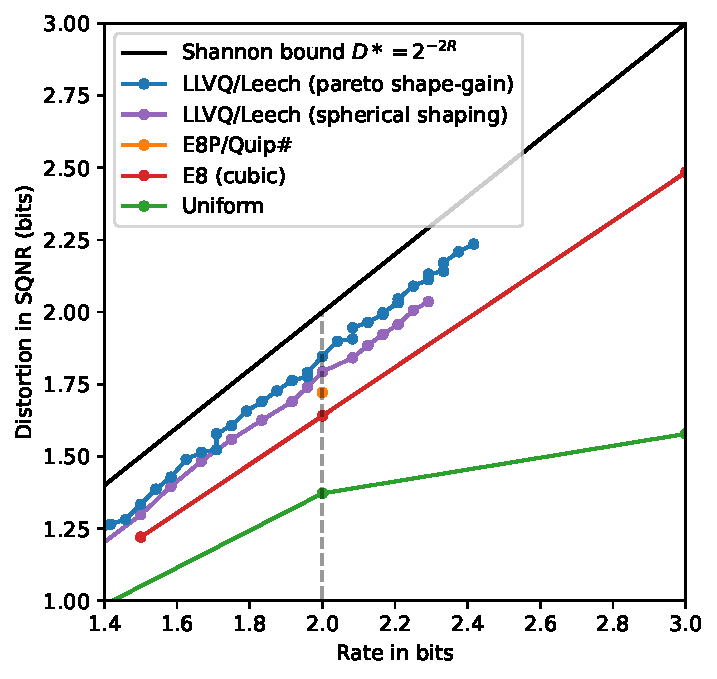
\includegraphics[width=0.33\textwidth]{figures/sqnr-plot.pdf}
    \vspace{-1em}
        \caption{$\widehat{\text{SQNR}}_{\text{bits}}$ versus bitrate (bits/dim) on Gaussian source.}
    \label{fig:rate_distortion}
    \vspace{-0.5em}
\end{figure}
\section{Performance on Idealistic Gaussian Source}


\subsection{Measured SQNR and Retention}

Due to structural constraints, practical quantizers inevitably fall below the theoretical limit. \autoref{fig:rate_distortion} shows the resulting SQNR versus bitrate behavior on an idealistic Gaussian source. Among the evaluated methods, our LLVQ construction attains the highest empirical SQNR at each tested bitrate, consistently outperforming existing approaches and tracking the Shannon bound more closely than the baselines.

To quantify how close a given method comes to the Shannon bound, we report a retention score that measures the fraction of the optimal SQNR achieved at a given bitrate. At a fixed bitrate (e.g., $R=2$ bits/dim), we report the empirical MSE and SQNR (in bits), and quantify how close the quantizer is to the Shannon limit using a \emph{retention} score:
\begin{align}
\text{Ret} (\%) = \frac{\widehat{\text{SQNR}}_{\text{bits}}}{\text{SQNR}^*_{\text{bits}}(R)} {\times} 100
= \frac{\widehat{\text{SQNR}}_{\text{bits}}}{R} {\times} 100,
\end{align}
since conveniently $\text{SQNR}^*_{\text{bits}}(R)=R$, under our convention of measuring signal-to-noise in bits.

As summarized in Table~\ref{tab:gaussian_performance}, the empirical SQNR and retention scores at $R=2$~bits/dim reveal clear gaps in performance across quantizers. Uniform quantization performs worst, reflecting its known suboptimality in Gaussian sources, while structured lattice-based schemes such as cubically bounded E8 and E8P/Quip \# achieve notably higher retention. Our LLVQ constructions achieve the best performance, achieving MSE and SQNR closest to the Shannon limit. This shows that LLVQ uses the available bitrate more efficiently, yielding substantially lower distortion on Gaussian inputs than existing lattice-based approaches.


\begin{table*}[t]
\centering
\caption{Comparison with wider set of methods for quantizing Llama-v2 7B model using different quantization methods, evaluated by wikitext-2 (Wiki) perplexity at 4096 context length and downstream task performance (CSR and MMLU), comparing results in literature. LLVQ consistently outperforms standard vector quantization approaches in performance against bits per parameter (Bits).}
\vspace{-0.5em}
\label{tab:ptq-performance-literature}
\resizebox{\linewidth}{!}{
\begin{tabular}{l l r c c | c c c c c c c }
& & & & & \multicolumn{7}{c}{Llama-2 7B} \\
\textbf{Method} & \textbf{Details} (from literature) & \textbf{Finetuned} & \textbf{LM Eval} & \,\textbf{BPW}\, &
\textbf{Wiki} $\downarrow$ %\textbf{MMLU}
& \textbf{Arc-C} $\uparrow$  & \textbf{Arc-E} $\uparrow$ & \textbf{BoolQ} $\uparrow$ & \textbf{Winogrande} $\uparrow$ & \textbf{Hellaswag} $\uparrow$ & \textbf{PiQA} $\uparrow$ \\
\hline
Baseline & (\textbf{Ours}) & - & acc & 16 & 5.11
%45.85
& \textbf{43.2} & \textbf{75.6} & \textbf{79.3} & \textbf{69.9} & \textbf{57.1} & \textbf{78.1}  \\
\hline
Quip\# & Tables 4 \& 10 of Quip\# paper & No & acc/acc\_norm & 2 & 8.22 & 32.5 & 42.8 & 62.3 & 62.4 & - & 71.2 \\ %\hline
%GPTVQ & Table 10 of GPTQ paper & not reported & acc\_norm & 2.125 & - & 34.4 & 60.4 & 65.5 & 65.0 & 64.0 & 73.3 \\
\hline
%LLVQ (\textbf{Ours}) & $\text{norm}(\Lambda_{24}(13))$+0 bit gain & 2 & No & acc & 2 & & \textbf{38.9} & \textbf{72.5} & - & - & \textbf{50.9} & \textbf{75.6} \\
% LLVQ (\textbf{Ours}) & 
% [spherical shaping]
% & 2 & No & acc & 2 & & \\
LLVQ (\textbf{Ours}) &
[spherical shaping]
& No & acc & 2 & 7.61 & 34.7 & 69.3 & 67.5 & 64.6 & 46.6 & 73.5 \\
LLVQ (\textbf{Ours}) &
[shape-gain, 2 bit gain]
& No & acc & 2 & \textbf{6.83} & 
\textbf{35.5} & \textbf{69.8} & \textbf{73.0} & \textbf{66.9} & \textbf{49.7} & \textbf{75.2} \\
% LLVQ (\textbf{Ours}) & 
% [shape-gain, 0 bit gain]
% %$\text{norm}(\Lambda_{24}(13))$+0 bit gain
% & 2 & No & acc & 2 & & \textbf{38.9} & \textbf{72.5} & \textbf{70.4} & \textbf{65.8} & \textbf{50.9} & \textbf{75.6} \\
% LLVQ (\textbf{Ours}) &
% [shape-gain, 2 bit gain]
% %$\text{norm}(\Lambda_{24}(11))$+2 bit gain
% & 2 & No & acc & 2 & & \textbf{38.8} & \textbf{71.8} & \textbf{73.7} & \textbf{67.6} & \textbf{51.1} & \textbf{76.0} \\
\hline
\hline
Quip &  Table 3 of Quip\# paper & Yes & acc & 2 & - & 19.4 & 26.0 & 54.6 & 51.8 & - & - \\
OmniQ & Table 3 of Quip\# paper & Yes & acc & 2 & - & 21.6 & 35.2 & 57.5 & 51.5 & - & - \\
%AQLM &  Table 3 of Quip\# paper & Yes & acc & 2.07 & - & 33.6 & 62.8 & 73.5 & 64.6 & - & - \\
%Quip\# & Table 3 of Quip\# paper & Yes* & acc & 2 & - & 34.6 & 64.6 & 75.1 & 64.9 & - & - \\
%Quip\# & Table 10 of Quip\# paper & Yes & acc & 2 & - & - & - & 68.3 & 64.9 & - & - \\
%Quip\# & Table 10 of Quip\# paper & Yes & acc\_norm & 2 & - & 36.1 & 50.5 & - & - & - & 74.9 \\
AQLM & Tables 5 \& 6 of QTIP paper & Yes & not reported & 2.07 & 6.93 & 32.8 & 63.7 & 74.8 & 65.7 & - & - \\
Quip\# & Tables 5 \& 6 of QTIP paper & Yes & not reported & 2 & 6.19 & 35.2 & 65.3 & 75.4 & 64.9 & - & - \\
QTIP & Tables 5 \& 6 of QTIP paper & Yes & not reported & 2 & 5.86 & 35.7 & 65.6 & \textbf{75.9} & 64.7 & - & - \\
PV-tuning & Table 8 of PV-tuning paper & Yes & acc & 2 & 5.84 & 38.4 & 71.2 & - & \textbf{66.7} & 53.5 & 77.0 \\
\hline
LLVQ (\textbf{Ours}) &
[spherical shaping]
& Yes & acc & 2 & \textbf{5.60} & \textbf{40.6} & \textbf{72.9} & 70.9 & 65.1 & 52.5 & 75.5 \\
LLVQ (\textbf{Ours}) &
% [shape-gain, 2 bit gain]
% LLVQ (\textbf{Ours}) &
% % $\text{norm}(\Lambda_{24}(13))$+0 bit gain
% [shape-gain, 0 bit gain]
% & Yes & acc & 2 & & \textbf{39.9} & \textbf{73.7} & 74.1 & 66.5 & \textbf{53.6} & 76.2 \\
% LLVQ (\textbf{Ours}) &
% % $\text{norm}(\Lambda_{24}(11))$+2 bit gain
[shape-gain, 2 bit gain]
& Yes & acc & 2 & \textbf{5.48} & \textbf{39.8} & \textbf{72.9} & 75.3 & 66.3 & \textbf{54.1} & \textbf{77.1} \\
\hline
\end{tabular}
}
\vspace{-1.0em}
\end{table*}

\begin{table}[h]
\centering
\caption{Ablation study with and without Hadamard rotations, evaluated on wikitext-2 perplexity (PPL) and downstream tasks (CSR and MMLU). LLVQ consistently outperforms standard VQ approaches in performance against bits per weight (BPW).}
\label{tab:hadamard-ablation}
\resizebox{\linewidth}{!}{
\begin{tabular}{l | c c l | c c c }% | c c c | c c c }
& & & & \multicolumn{3}{c}{Llama-2 7B} \\
\textbf{Method} \small{(no finetune)} & \textbf{Dim}&
%\textbf{Dtype}
\footnotesize{\textbf{BPW}} & %\textbf{\footnotesize{Hessian}}
\textbf{Hadamard}
& \textbf{Wiki} $\downarrow$ & \textbf{MMLU} $\uparrow$ & \textbf{CSR} $\uparrow$ \\
\hline
Baseline & 1 %\footnotesize{(scalar)}
& 16 & - & 5.12 & 45.7 & 70.4 \\
\hline
Integer (GPTQ) & 1 %\footnotesize{(scalar)} 
%int2
& 2
%\checkmark
& No Rotation & 
3411.6 & 26.6 & 39.7 \\
Integer (Quarot) & 1 & %\footnotesize{(scalar)} &
%int2
2 & 
%\checkmark
Input & 41.87 & 27.0 & 41.7 \\
Integer & 1 %\footnotesize{(scalar)}
&
%int2
2 &
%\checkmark
\small{Input + Output} &
37.83 & 26.1 & 48.4
\\
\cdashline{0-6}[5pt/4pt] 
E8P & 8 &
2 &
%\checkmark 
No Rotation & 105.98 & 24.8 & 44.9 \\
E8P & 8 & 
2 &
%\checkmark
Input & 9.24 & 31.0 & 59.8 \\
E8P (Quip\#) & 8 &
%e8p12
2 &
% \checkmark
\small{Input + Output} & 7.96 & 30.5 & 61.4
\\
\cdashline{0-6}[5pt/4pt] 
% LLVQ (?) & (\textbf{Ours}) & 24 & leech2 & 2 & \checkmark & No Rotation & 19.073(c) & 24.989 & 51.115 \\
% LLVQ (?) & (\textbf{Ours}) & 24 & leech2 & 2 & \checkmark & Input & 7.518 & 30.338 & 61.473 \\
% LLVQ (?) & (\textbf{Ours}) & 24 & leech2 & 2 & \checkmark & Input + Output & 7.024 & 26.933 & 60.616 \\
\cdashline{0-6}[5pt/4pt] 
LLVQ [spherical shaping] %(\textbf{Ours})
& 24 & 2 &
%\checkmark 
No Rotation & 191.90 & 24.0 & 53.5 \\
LLVQ [spherical shaping] %(\textbf{Ours})
& 24 & 2 & %\checkmark 
Input & \textbf{6.80} & \textbf{35.1} & \textbf{65.4}
 \\
LLVQ [spherical shaping] % (\textbf{Ours})
& 24 & 2 &
%\checkmark 
\small{Input + Output} & \textbf{7.61} & \textbf{33.4} & \textbf{62.1} \\
\cdashline{0-6}[5pt/4pt] 
LLVQ [shape-gain] % (\textbf{Ours}) 
& 24 & 2 & 
%\checkmark 
No Rotation & \textbf{7.27} & \textbf{29.8} & \textbf{61.5} \\
LLVQ [shape-gain] % (\textbf{Ours})
& 24 & 2 &
%\checkmark 
Input & 
\textbf{6.90} & \textbf{36.0} & \textbf{63.6}
\\
LLVQ [shape-gain] %(\textbf{Ours})
& 24 & 2 &
%\checkmark
\small{Input + Output} & \textbf{6.83} & \textbf{34.9} & \textbf{64.6}
 \\
\hline
\end{tabular}
}
%\vspace{-1.5em}
\end{table}

\section{LLM Quantization Results}

\subsection{Experimental Set-up}

For empirical results, we compute (GPTQ-style) layer-wise Hessians on 6,100 sequences from DCLM-edu \citep{li2024datacomp,allal2025smollm2}, matching the calibration set size used in prior work \citep{tseng2024quip}. When finetuning is applied, we update only the input scales, scalars shared across rows, which add a negligible number of bits per weight and introduce relatively little risk of overfitting.

\subsection{PTQ Results (Own Pipeline)}

We begin by evaluating post‑training quantization (PTQ) using a unified quantization pipeline enabling a strict apples‑to‑apples comparison across methods. Table~\ref{tab:other-models} summarizes PTQ results on Llama‑2 7B, Llama-3 8B, Ministral-3 8B, and Qwen‑v3 4B and 8B under this setup. The gap between scalar baselines (RTN, GPTQ \citep{frantar2022gptq}, Quarot \citep{ashkboos2024quarot}) and higher‑dimensional VQ methods is immediately evident: naive 2‑bit RTN yields extremely high perplexity and severe task degradation, while GPTQ and Quarot improve stability through Hessian curvature and Hadamard rotations, yet remain constrained by the limited representational capacity of 1D quantization.

Higher‑dimensional approaches, such as Quip\#, substantially reduce this gap. However, our LLVQ method, employing Leech‑lattice‑based 24‑dimensional vector quantization, consistently achieves the strongest 2‑bit performance across all metrics. Wikitext perplexity, MMLU accuracy, and CSR all show clear gains over Quip\#, demonstrating that high‑dimensional structured lattices provide markedly more efficient weight‑space packing than both scalar and E8‑based quantizers.
 

\subsection{Impact of Hadamard Rotations}

Following recent quantization literature \citep{ashkboos2024quarot, chee2023quip}, we reparameterize the weights of each linear layer, using randomized Hadamard transforms on the input and output as in \citep{tseng2024quip}. The goal of such transformations is to preserve the model’s functional output while making the marginal weight statistics more Gaussian‑like, reducing outliers, and making them substantially easier to quantize. Table~\ref{tab:hadamard-ablation} examines the impact of Hadamard-based input/output rotations across three quantizer families: scalar integer methods (GPTQ/Quarot), the E8P/Quip\# codebook, and the proposed LLVQ quantizers based on the Leech lattice. Across all methods, the “Input + Output” rotation consistently delivers the best downstream performance, confirming the value of decorrelating activation and weight spaces prior to quantization. Scalar integer quantization benefits the most from rotations due to the minimal flexibility of 1D codebooks.

Interestingly, although rotations consistently improve performance, LLVQ with shape–gain and spherical GPTQ even \textit{without} rotations performs remarkably well, even surpassing the performance of Quip\#'s E8P codebook \textit{with} rotations, using consistent quantization pipeline without finetuning. This suggests that higher‑dimensional vector quantization intrinsically reduces the relience on rotational preprocessing. This is especially relevant because, although rotational preprocessing can often be fused or merged into the model \citep{ashkboos2024quarot,van2025fptquant}, this is not always possible. In such cases, these transformations must be applied online, adding latency and computational overhead. The results therefore indicate that higher‑dimensional vector quantization methods, such as LLVQ, can mitigate or even eliminate the need for expensive rotational preprocessing (e.g., online Hadamards), while still achieving state‑of‑the‑art quantization quality.

\subsection{Comparison to Results in Literature}

In addition to the unified PTQ evaluation presented earlier, where all methods are assessed under the exact same pipeline for strict apples‑to‑apples comparison, Table~\ref{tab:ptq-performance-literature} further broadens the analysis to include results previously reported in the literature. Although published baselines such as OmniQ, AQLM, Quip\#, and QTIP may slightly differ in training conditions, calibration set composition, and dataset sizes, these comparisons remain highly meaningful, as they contextualize performance across independent pipelines.

Optionally, we incorporate a lightweight fine‑tuning step that learns an element‑wise multiplicative correction on the inputs of each linear layer, following \citep{tseng2024quip}; equivalently, this can be viewed as learning per‑column scaling factors for the weight matrices. Because these scalars are shared across rows, the overhead is negligible (less than $0.001$ bits per weight even in full 32‑bit precision). We train only these scale parameters for a short run of roughly 1M tokens. This minimal adaptation reliably improves perplexity, MMLU, and CSR across quantization methods, acting as a lightweight alignment step. 

Notably, LLVQ maintains a clear advantage compared to the strongest results reported across the broader literature. Crucially, LLVQ \textit{without} any fine‑tuning is competitive, sometimes surpassing, the performance of the best baselines \textit{with} fine‑tuning. This despite using a very strict definition of “no fine‑tuning” for our own method, meaning that all corrections arise solely from layer‑local, Hessian‑based updates derived from activation statistics, with no reliance on gradient updates, such as the inter‑layer fine‑tuning used in Quip\# and QTIP, and without any end‑to‑end tuning of the quantized model. Overall, LLVQ achieves state‑of‑the‑art performance in a strictly PTQ setting, outperforming methods that rely on additional fine‑tuning for recovery. When fine‑tuning is added (for LLVQ, only shared row-/column-wise scale terms), the performance gap widens further, yielding results close to the baseline model (2.5\%–7.6\% degradation in benchmark accuracies), pushing the frontier of practical LLM quantization into the ultra‑low‑bitrate regime of just 2 bits per weight.

\section{Conclusion}

We introduced \emph{Leech Lattice Vector Quantization} (LLVQ), a practical high-dimensional vector quantizer, grounded in the geometric and combinatorial structure of the Leech lattice. LLVQ provides an expressive and computationally efficient alternative to conventional scalar and low-dimensional vector quantizers. Our contributions include: (i) an extended shell-based search procedure supporting multi-shell codes, (ii) a fully invertible indexing scheme enabling codebook-free quantization and dequantization, and (iii) demonstrating Leech-lattice-based vector quantization of LLMs.

Experimentally, LLVQ achieves state-of-the-art performance in both idealized and practical settings. On Gaussian sources, LLVQ realizes the highest SQNR among competing quantizers, achieving over 92\% retention of the Shannon limit at 2~bits/dim. On all assessed large language models of the Llama-2 and Llama-3, Ministral-3, and Qwen-v3 model families, LLVQ consistently outperforms existing PTQ baselines such as AQLM, Quip\# and QTIP across perplexity and downstream task performance. This shows that the theoretical benefits of high-dimensional lattices on Gaussian data translates to practical benefits for modern LLM compression. 

%For real-world utility we do note some practical considerations, such as implied vector dimension of 24 being less convenient than a power of 2.

%These results highlight the advantages of high-dimensional lattice structures for neural compression, particularly in regimes where scalar methods fail to maintain accuracy.

Overall, LLVQ demonstrates that high-dimensional lattices offer substantial benefits for modern neural network compression. We hope this work inspires further exploration of mathematically grounded quantization schemes for scalable and efficient large model deployment.

% In the unusual situation where you want a paper to appear in the
% references without citing it in the main text, use \nocite
%\nocite{langley00}

\newpage
\bibliography{example_paper}
\bibliographystyle{icml2026}


%%%%%%%%%%%%%%%%%%%%%%%%%%%%%%%%%%%%%%%%%%%%%%%%%%%%%%%%%%%%%%%%%%%%%%%%%%%%%%%
%%%%%%%%%%%%%%%%%%%%%%%%%%%%%%%%%%%%%%%%%%%%%%%%%%%%%%%%%%%%%%%%%%%%%%%%%%%%%%%
% APPENDIX
%%%%%%%%%%%%%%%%%%%%%%%%%%%%%%%%%%%%%%%%%%%%%%%%%%%%%%%%%%%%%%%%%%%%%%%%%%%%%%%
%%%%%%%%%%%%%%%%%%%%%%%%%%%%%%%%%%%%%%%%%%%%%%%%%%%%%%%%%%%%%%%%%%%%%%%%%%%%%%%
\newpage
\appendix
\onecolumn

% ====== PREAMBLE REQUIREMENTS ======
% \usepackage{amsmath, amssymb}
% \usepackage{pgfplots}
% \pgfplotsset{compat=1.18}
% \usepackage{siunitx} % optional, for \SI{}{} units



\hspace{5em}

\newpage
\section{Pseudo-code}

% \subsection{Quantization kernel}
% 
% Work in progress...
% 
% \begin{algorithm}[H]
% \caption{Quantization kernel (\textbf{ours})}
% \begin{algorithmic}[1]
% \Require Vector $w \in \R^d $
% % \State Find smallest leader $l$ for which $i < \tilde{N}(l)$
% % \State Compute leader-local subindex $i_{\text{leader}} = i - \tilde{N}(l-1)$
% % \If{leader $l$ is even}
% %     \State Compute Golay index $i_{\text{golay}} = i_{\text{leader}} ... $
% %     \State Compute permutation index $i_{\text{perm}} = i_{\text{leader}} ...$
% %     \State Compute Golay mask $g \in \{0,1\}^{24}$
% %     \State Partition leader into mod-4 classes
% %     \State Unrank permutations for each class
% %     \If{check sign parity}
% %         \State Flip sign of element with ...
% %     \EndIf
% % \Else
% %     \State Compute Golay index $i_{\text{golay}} = i_{\text{leader}} ... $
% %     \State Compute permutation index $i_{\text{perm}} = i_{\text{leader}} ...$
% %     \State Compute Golay mask $g \in \{0,1\}^{24}$
% %     \State Unrank full multiset permutation (4096 options)
% % \EndIf
% \State \Return Quantized vector $\hat{w} \in \Lambda_{24}(m)$ and associated index $i_{\hat{w}} \in [1, N(m)]$ \\
% Work in progress...
% \end{algorithmic}
% \label{alg:quantization-kernel}
% \end{algorithm}
% 
% \subsection{Dequantization kernel}
% 
% \begin{algorithm}[H]
% \caption{Dequantization kernel (\textbf{ours})}
% \begin{algorithmic}[1]
% \Require Global index $i \in [0, \dots, N(m)] $ \\
% % \State Find smallest leader $l$ for which $i < \tilde{N}(l)$
% % \State Compute leader-local subindex $i_{\text{leader}} = i - \tilde{N}(l-1)$
% % \If{leader $l$ is even}
% %     \State Compute Golay index $i_{\text{golay}} = i_{\text{leader}} ... $
% %     \State Compute permutation index $i_{\text{perm}} = i_{\text{leader}} ...$
% %     \State Compute Golay mask $g \in \{0,1\}^{24}$
% %     \State Partition leader into mod-4 classes
% %     \State Unrank permutations for each class
% %     \If{check sign parity}
% %         \State Flip sign of element with ...
% %     \EndIf
% % \Else
% %     \State Compute Golay index $i_{\text{golay}} = i_{\text{leader}} ... $
% %     \State Compute permutation index $i_{\text{perm}} = i_{\text{leader}} ...$
% %     \State Compute Golay mask $g \in \{0,1\}^{24}$
% %     \State Unrank full multiset permutation (4096 options)
% % \EndIf
% Work in progress...
% \State \Return (De)quantized vector $\hat{w} \in \Lambda_{24}(m) $
% \end{algorithmic}
% \label{alg:dequantization-kernel}
% \end{algorithm}

\subsection{Overall Shape-gain Quantization with Hessian Corrections}

\begin{algorithm}[H]
\caption{Overall Shape-gain Quantization with Hessian Corrections}
\begin{algorithmic}[1]
\For{each layer $l$ in model}
    \State Estimate Hessian matrix $\mH$ using layer inputs $\mX$ (\autoref{subsec:hessian_correction})
    \State Partition each row of weight matrix $W_l \in \mathbb{R}^{N \times D}$ into $G$ partitions: $\mathbf{v}_1, \mathbf{v}_2, \dots, \mathbf{v}_G$ where $G = D/24$.
    \For{group index $g = 1$ to $G$}
        \State Extract submatrix $V_g \in \mathbb{R}^{N \times 24}$ containing all $\mathbf{v}_g$ across rows
        \For{each vector $\mathbf{v}_g^{(i)}$ in $V_g$} (in parallel)
            \State Compute direction $\hat{\mathbf{v}}_g^{(i)} = \mathbf{v}_g^{(i)} / \|\mathbf{v}_g^{(i)}\|$
            \State Compute scale $s_g^{(i)} = \|\mathbf{v}_g^{(i)}\|$
            \State Find nearest Leech lattice point $\mathbf{q}_g^{(i)}$ maximizing $\cos(\theta) = \hat{\mathbf{v}}_g^{(i)\top} \mathbf{q}_g^{(i)}$ (\autoref{sec:nearest-leech})
            \State Optionally quantize $s_g^{(i)}$ using scalar quantizer
            \State Update residual: $\mathbf{v}_{g,\text{res}}^{(i)} = \mathbf{v}_g^{(i)} - s_g^{(i)} \cdot \mathbf{q}_g^{(i)}$
        \EndFor
        \State In-place adjust $W_l$ using residual $V_g$ and Hessian $\mH$ (Hessian correction, \autoref{sec:hessian_correction})
    \EndFor
\EndFor
\end{algorithmic}
\end{algorithm}



\newpage
\section{Shape-Gain Quantization and Constructing Spherical Codes from Lattices}
\label{sec:shape-gain}

An alternative to spherical shaping, where all lattice points within a prescribed radius are taken as the finite quantization grid, is \textit{shape–gain} quantization \citep{sabin1982product,hamkins2002gaussian,gersho2012vector}. In shape–gain, the magnitude of a vector (its “gain”) is quantized separately using a standard scalar quantizer, while its direction (its “shape”) is quantized using a spherical quantizer defined over a spherical code, i.e., a finite subset of points on the high‑dimensional unit sphere. Although this approach is slightly more involved than spherical shaping, as it requires two quantizers rather than one, it can yield superior rate–distortion performance for Gaussian sources, as we demonstrate in \autoref{app:spherical-bounding-vs-shape-gain}.

More formally, shape–gain quantization considers (polar-)decomposing each vector into its \emph{shape} (direction) and \emph{gain} (magnitude). Any non-zero vector $\mathbf{x}\in\mathbb{R}^n$ can be written as
\begin{align}
\mathbf{x} = r\,\mathbf{u},
\qquad
r=\|\mathbf{x}\| \in \R,\;\; \mathbf{u}=\mathbf{x}/\|\mathbf{x}\|\in\mathbb{S}^{n-1}.
\end{align}
Quantization then treats $r$ and $\mathbf{u}$ separately, so that the overall code becomes the Cartesian product of a scalar quantizer on $\mathbb{R}$ and a quantizer on the sphere $\mathbb{S}^{n-1}$. For Gaussian sources, this factorization is particularly appealing: the gain $r$ follows a root chi‑square distribution (since $r^2 \sim \chi^2_n$), which can be accurately quantized using an analytically tractable inverse CDF. The core design challenge therefore lies in constructing expressive, approximately uniformly distributed, and high‑rate spherical codes, together with algorithms that efficiently map a vector to its nearest code point on the sphere and represent that point using a compact index.

\paragraph{Spherical codes}

A spherical code is formally defined as a $(d, N, s)$-code: a collection of $N$ points on the sphere $S^{d-1}$ such that the inner product between any two distinct points is at most $s$. An optimal $(d, N, s)$-code is one for which no $(d, N_0, s)$-code with $N_0 > N$ exists. Among the most celebrated examples are the minimal vectors of the $E_8$ and Leech lattices, which yield an $(8, 240, \tfrac{1}{2})$-code and a $(24\; 196{,}560, \tfrac{1}{2})$-code, respectively. Their optimality was established by \citet{kabatiansky1978bounds, odlyzko1979new}, and their uniqueness by \citet{bannai1981uniqueness}. These spherical codes also solve the kissing number problem in their respective dimensions, achieving $240$ contacts in $\mathbb{R}^8$ and $196{,}560$ in $\mathbb{R}^{24}$ \citep{ericson2001codes, conway2013sphere}.

Despite their optimality, the first shells of $E_8$ and the Leech lattice contain too few points to serve as high-bitrate spherical codes: $\log_2(240)/8 \approx 1$ bit/dim for $E_8$ and $\log_2(196{,}560)/24 \approx 0.73$ bit/dim for the Leech lattice. Such bitrates are insufficient for practical neural network quantization, which typically operates in the 2--3 bits/dim or higher (up to 16) range. To obtain richer directional codebooks, we consider a normalized spherically bounded subset of the Leech lattice, i.e., the union of all lattice points within a chosen radius, which forms a dense spherical code after normalization. These multi-shell Leech-based codes serve as the foundation for our angular quantization scheme. Their geometric uniformity minimizes directional distortion, and their high density supports bitrates compatible with modern compression and quantization needs. When combined with an appropriate scalar quantizer for the gain, the resulting shape-gain quantizer performs well not only for ideal Gaussian sources but also for real-world neural network weight distributions.



\newpage
\section{Quantizer/dequantizer block diagrams}
\label{sec:qd-blocks}

We quantize a vector $\mathbf{w}\in\mathbb{R}^d$ using a mapping $q:\mathbb{R}^d\to[1,N(m)]$, where the integer index range $[1,N(m)]$ is sized such that $\log_2(N(m))/24$ equals the desired bits per dimension. The quantizer output is $i_{\hat{\mathbf{w}}}=q(\mathbf{w})$, and the reconstruction is obtained via the dequantizer $\text{Dequantizer}:[1,N(m)]\to\mathbb{R}^d$, yielding $\hat{\mathbf{w}}=\text{Dequantizer}(i_{\hat{\mathbf{w}}})$. This abstraction covers a family of encoders with geometric preprocessing (e.g., shaping or factorization) followed by index selection, and a corresponding inverse mapping at the decoder.

\paragraph{Spherical shaping.}
Figure~\ref{fig:diagram1} depicts the \emph{spherical shaping} variant based on a ball cut of the Leech lattice. The vector $\mathbf{w}$ is first projected into a spherical shaping region, typically the Euclidean ball $\mathbb{B}(0,R)$, and the index is selected by nearest-neighbor search over $\Lambda_{24}\cap\mathbb{B}(0,R)$:
\[
    i_{\hat{\mathbf{w}}}=q(\mathbf{w})
    = \arg\min_{i:\,\mathbf{c}_i\in\Lambda_{24}\cap\mathbb{B}(0,R)}\|\mathbf{w}-\mathbf{c}_i\|_2^2,
    \qquad
    \hat{\mathbf{w}}=\mathbf{c}_{i_{\hat{\mathbf{w}}}}.
\]
This realizes high shaping efficiency while enforcing a finite-energy codebook.

\begin{figure}[h!]
    \centering
    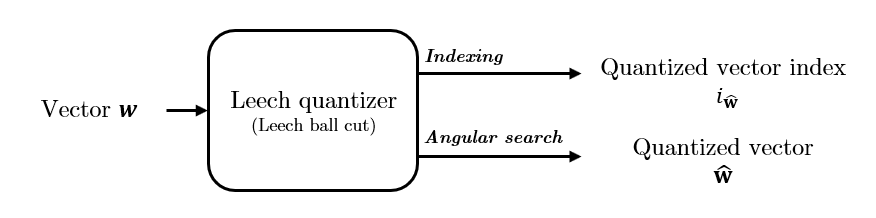
\includegraphics[width=0.80\linewidth]{figures/diagram1.png}
    \caption{Spherical shaping: ball cut of the Leech lattice with nearest-neighbor selection over $\Lambda_{24}\cap\mathbb{B}(0,R)$.}
    \label{fig:diagram1}
\end{figure}

\paragraph{Shape--gain.}
In the \emph{shape--gain} framework, $\mathbf{w}=g\,\mathbf{s}$ with $g=\|\mathbf{w}\|_2$ and $\mathbf{s}=\mathbf{w}/\|\mathbf{w}\|_2\in\mathbb{S}^{d-1}$. The independent variant in Fig.~\ref{fig:diagram3} applies separate quantizers to shape and gain,
\[
    i_{\hat{\mathbf{w}}}=q(\mathbf{w})
    = \big(q_{\mathrm{shape}}(\mathbf{s}),\,q_{\mathrm{gain}}(g)\big)\in[1,N(m)],
\]
and the dequantizer reconstructs $\hat{\mathbf{s}}$ and $\hat{g}$ and returns $\hat{\mathbf{w}}=\hat{g}\,\hat{\mathbf{s}}$. While computationally simple, independence may induce norm mismatch because angular errors perturb the effective magnitude.

\begin{figure}[h!]
    \centering
    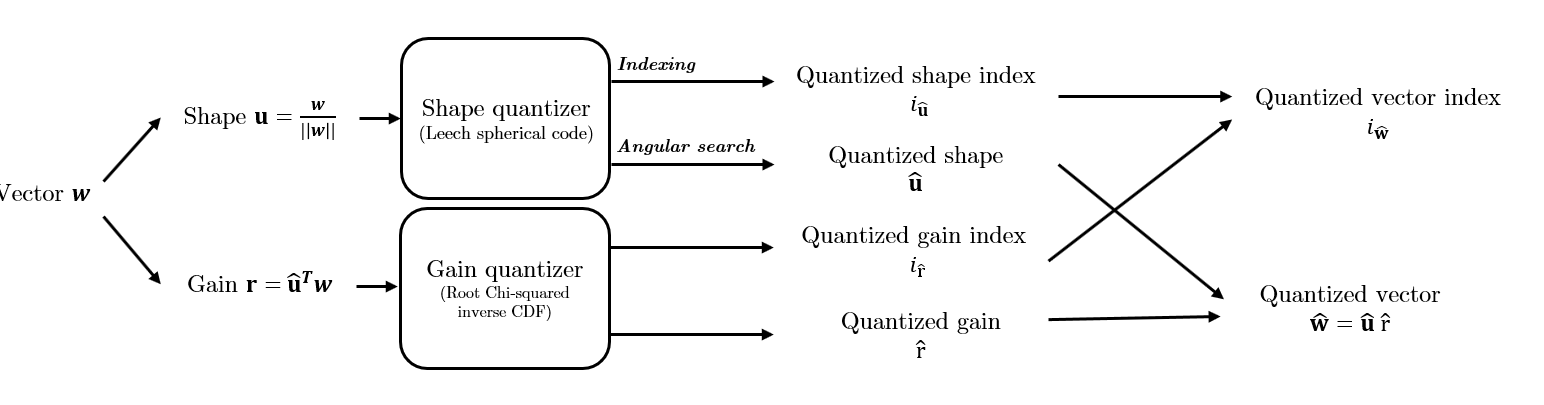
\includegraphics[width=0.80\linewidth]{figures/diagram3.png}
    \caption{Shape--gain with independent quantization of shape $\mathbf{s}$ and gain $g$, producing an index in $[1,N(m)]$ and reconstruction $\hat{\mathbf{w}}=\hat{g}\,\hat{\mathbf{s}}$.}
    \label{fig:diagram3}
\end{figure}

To mitigate this, Fig.~\ref{fig:diagram2} implements \emph{shape--gain with optimal scales} (post-shape gain optimization). After selecting the shape index, the quantized direction $\hat{\mathbf{s}}$ is known; the encoder computes
\[
    \gamma^\star=\langle \mathbf{w},\hat{\mathbf{s}}\rangle,
    \qquad
    i_{\hat{\mathbf{w}}}
    = \big(q_{\mathrm{shape}}(\mathbf{s}),\,q_{\mathrm{gain}\mid\hat{\mathbf{s}}}(\gamma^\star)\big)\in[1,N(m)],
\]
and the dequantizer mirrors this conditional mapping to obtain $\hat{g}$ and reconstruct $\hat{\mathbf{w}}=\hat{g}\,\hat{\mathbf{s}}$. Unless stated otherwise, this \emph{shape--gain with optimal scales} configuration is the one used in our main LLVQ experiments due to its superior rate--distortion behavior.

\begin{figure}[h!]
    \centering
    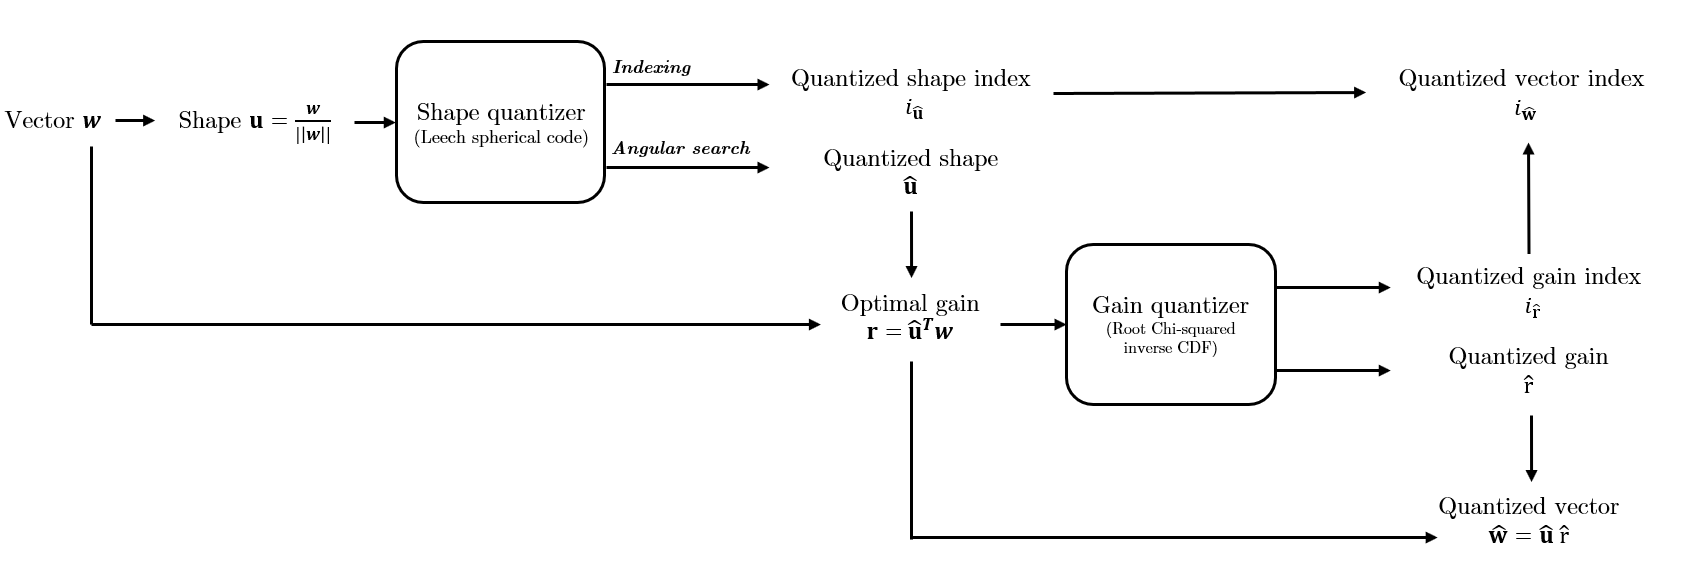
\includegraphics[width=0.80\linewidth]{figures/diagram2.png}
    \caption{Shape--gain with optimal scales: post-shape gain optimization via a shape-conditioned gain quantizer.}
    \label{fig:diagram2}
\end{figure}

\paragraph{Dequantizer.}
Given the integer index $i_{\hat{\mathbf{w}}}\in[1,N(m)]$, the dequantizer in Fig.~\ref{fig:diagram4} maps back to $\mathbb{R}^d$ by retrieving the appropriate representatives (lattice point or shape/gain codewords) and recombining them:
\[
    \text{Dequantizer}:[1,N(m)]\to\mathbb{R}^d,\qquad \hat{\mathbf{w}}=\text{Dequantizer}(i_{\hat{\mathbf{w}}}).
\]
This guarantees consistency with the encoder’s shaping or factorization policy.

\begin{figure}[h!]
    \centering
    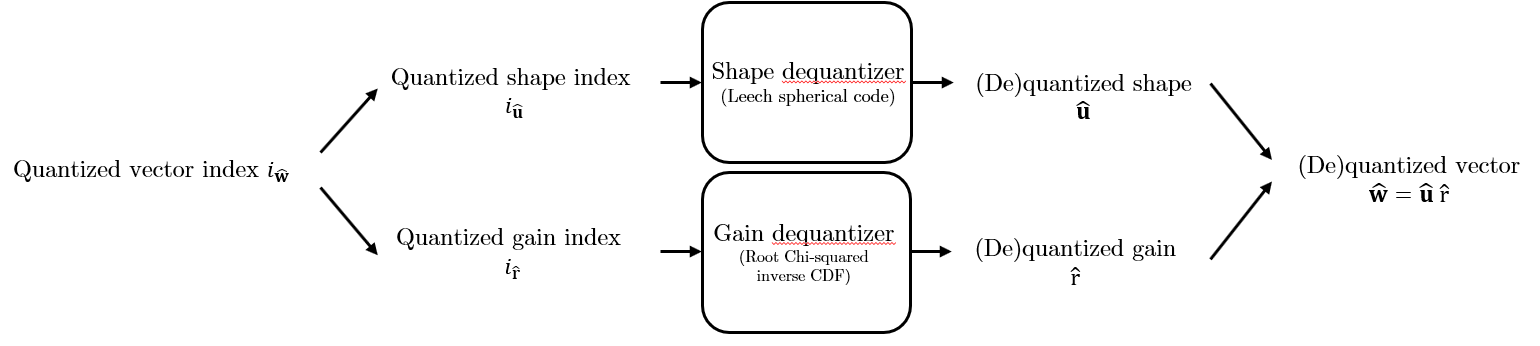
\includegraphics[width=0.80\linewidth]{figures/diagram4.png}
    \caption{Dequantizer mapping the integer index $i_{\hat{\mathbf{w}}}\in[1,N(m)]$ to the reconstruction $\hat{\mathbf{w}}\in\mathbb{R}^d$.}
    \label{fig:diagram4}
\end{figure}

A detailed comparison between spherical shaping and shape--gain is provided in Appendix~\ref{app:spherical-bounding-vs-shape-gain}. There, we found shape--gain to yield improved performance over spherical shaping, when using the Leech lattice; accordingly, we adopt the shape--gain with optimal scales scheme in our main LLVQ experiments unless explicitly noted otherwise.













\newpage
\section{Algorithm specification}

\noindent
\subsection{Optimal scales under shape-gain}

An additional benefit of spherical vector quantization (shape-gain) is that it renders the quantizer scale invariant: $q(s\vw) = q(\vw)$ for all $s \in \mathbb{R}$, so the scaled grid $q'(\vw) = \beta \cdot q(\vw / \beta)$ simplifies to $q'(\vw) = \beta \cdot q(\vw)$. This removes the need for line search and yields closed-form scale solutions. For the optimal scale that minimizes \textit{weight error} $\|\vw - \beta\,q(\vw)\|_2^2$, and with $\vq = q(\vw)$, we obtain
\begin{align}
\beta_* 
&= \arg\min_{\beta}\,\|\vw - \beta\,\vq\|_2^2
= \frac{\vq^\top \vw}{\vq^\top \vq}\,,
\end{align}
i.e., a projection of $\vw$ onto its quantized shape $\vq$. In the group-wise case, where weights are partitioned into blocks $\vw_i$, the same form applies per block: $\beta_i^* = \frac{q(\vw_i)^\top \vw_i}{q(\vw_i)^\top q(\vw_i)}$. Similarly, the optimal scale that minimizes \emph{output activations} can also be found in closed-form. We consider the matrix-vector product $W x = \sum_{i=1}^{G} \vw_i x_i$ with $G$ input channels or blocks. We approximate this as $\sum_{i=1}^{G} \beta_i\,q(\vw_i)\,x_i$, and define $\mA = [\,q(\vw_1)x_1,\ldots,q(\vw_G)x_G\,] \in \mathbb{R}^{B \times G}$ and $\vb = \mW\vx \in \mathbb{R}^B$. The optimal group-wise scale reduces to the least-squares solution:
\begin{align}
\boldsymbol{\beta}_*
&= \arg\min_{\boldsymbol{\beta}}\,\|\vb - \mA\,\boldsymbol{\beta}\|_2^2 \nonumber \\ 
%&= (\mA^\top \mA)^{-1} \mA^\top \vb
&= (\mA^\top \mA)^{-1} \mA^\top \mW\vx\,.
\end{align}
% The respective closed-form solutions for weight and activation space proxy losses are:
% \begin{align}
% \displaystyle \beta_* &= \arg\min_{\beta}\|\vw - \beta\,q(\vw)\|_2^2 = \frac{q(\vw)^\top \vw}{q(\vw)^\top q(\vw)}, \\
% \displaystyle \boldsymbol{\beta}_* &= \arg\min_{\boldsymbol{\beta}}\,\big\|\mW\vx - \sum_{i=1}^{G} \beta_i\,q(\vw_i)\,x_i\big\|_2^2 = (\mA^\top \mA)^{-1} \mA^\top \mW\vx.
% \end{align}

\subsection{Hessian-based corrections}
\label{subsec:hessian_correction}
In post-training quantization, analytic correction steps are interleaved with quantization to compensate for errors introduced by already quantized weights by adjusting the remaining ones. Instead of full fine-tuning, these corrections rely on fast analytic solutions.

\paragraph{Local Hessian Corrections}
For a linear layer $\mathbf{y} = \mathbf{W}\mathbf{x}$ with quantized weights $q(\mathbf{W})$ and error $\Delta\mathbf{W} = q(\mathbf{W}) - \mathbf{W}$, it is common \citep{nagel2020up} to target expected output MSE of each layer as (local) proxy objective:
\begin{align}
\mathcal{L}_{\text{local}}
&= \mathbb{E}\big[\| \Delta\mathbf{W}\,\mathbf{x}\|^2\big]\ 
= \mathbb{E}\big[\mathbf{x}^\top \Delta\mathbf{W}^\top \Delta\mathbf{W}\,\mathbf{x}\big] \\
&= \mathrm{Tr}\!\big(\Delta\mathbf{W}\,\mathbf{H}_{\text{in}}\,\Delta\mathbf{W}^\top\big),
\quad \mathbf{H}_{\text{in}} = \mathbb{E}[\mathbf{x}\mathbf{x}^\top].
\end{align}
The equalities are exact under the true second moment; in practice we replace $\mH_{\text{in}}$ by the empirical estimator $\tilde{\mH}_{\text{in}} = \frac{1}{N} \mX^{\top}\mX$ from a finite calibration set $\mX \in \R^{N \times D_{\text{in}}}$, so the trace expression becomes a Monte Carlo (stochastic) approximation of the population objective, which converges to the exact one as $N \to \infty$ under standard i.i.d. assumptions (law of large numbers).
Rows of $\mathbf{W}$ are independent because the quadratic form decomposes as
\[
\mathcal{L}_{\text{local}} = \sum_{r} \Delta\mathbf{w}_r^\top \mathbf{H}_{\text{in}} \Delta\mathbf{w}_r,
\]
where $\Delta\mathbf{w}_r$ is the $r$-th row. For a single row, partition indices into \emph{changed} $C$ and \emph{remaining} $R$:
\[
\mathbf{H}_{\text{in}} =
\begin{bmatrix}
\mathbf{H}_{CC} & \mathbf{H}_{CR}\\
\mathbf{H}_{RC} & \mathbf{H}_{RR}
\end{bmatrix}, \quad
\Delta\mathbf{w} = [\Delta\mathbf{w}_C;\,\Delta\mathbf{w}_R].
\]
Minimizing the quadratic w.r.t.\ $\Delta\mathbf{w}_R$ gives the analytic correction:
\[
\boxed{\Delta\mathbf{w}_R^\star = -\,\mathbf{L}_{RR}^{-1}\,\mathbf{L}_{RC}\,\Delta\mathbf{w}_C.}
\]
where $\mL_{RR}$ and $\mL_{RC}$ are lower-triangular matrices by indexing Cholesky of $\mH$. Hence, the corrections require a single Cholesky decomposition, and a single lower-triangular solve, which has fast implementations. The correction algorithm is similar to LDLQ \citep{tseng2024quip}, generalizes the common GPTQ/OPTQ  \citep{frantar2022gptq} from scalar to vector quantization, and corrects updates in \citep{van2024gptvq} to account for column-mixing of VQ and typos. From a probabilistic perspective, it can be noted that the correction is equivalent to Gaussian conditioning where the conditional mean of remaining weights $R$ given the changed weights $C$, and Gaussian elimination. It is well-known that performing this iteratively can efficiently be done in Cholesky: the lower-triangular factor $\mathbf{L}$ from $\mathbf{H}_{\text{in}} = \mathbf{L}\mathbf{L}^\top$ as the inverse Cholesky only has to be computed ones and inverse Cholesky of remaining weights form a submatrix of the original inverse matrix. Batched triangular solves apply corrections for multiple rows efficiently.

% \paragraph{Global Hessian Quantization (LLM Surgeon, YAQA).}
% The target is the final loss, typically KL divergence between original and quantized outputs:
% \[
% \mathcal{L}_{\text{global}} \approx \mathrm{KL}\big(\mathbf{p}_{\text{orig}} \,\|\, \mathbf{p}_{\text{quant}}\big).
% \]
% A second-order expansion uses a Kronecker-factored Hessian:
% \[
% \mathbf{H} \approx \mathbf{H}_{\text{out}} \otimes \mathbf{H}_{\text{in}}, \quad
% \mathbf{H}_{\text{in}} = \mathbf{X}^\top\mathbf{X}, \;\mathbf{H}_{\text{out}} = \mathbf{G}^\top\mathbf{G}.
% \]
% Partitioning the vectorized weights into changed $C$ and remaining $R$ gives:
% \[
% \boxed{\Delta\mathbf{w}_R^\star = -\,\mathbf{H}_{RR}^{-1}\,\mathbf{H}_{RC}\,\Delta\mathbf{w}_C,}
% \]
% where blocks are taken from $\mathbf{H}\approx \mathbf{H}_{\text{out}}\otimes\mathbf{H}_{\text{in}}$. Efficient application uses Cholesky factors of $\mathbf{H}_{\text{in}}$ and $\mathbf{H}_{\text{out}}$ without forming $\mathbf{H}$ explicitly.
% 
% LLM Surgeon employs K-FAC to align the quadratic approximation with the final loss, while YAQA extends this approach to quantization and improves curvature quality by modeling attention mixing, using short calibration runs that collect both activations and gradients (TODO: assuming we'll use/ablate both local and global corrections?).

\emph{Local vs global.} Local updates can also be seen as targeting the final loss under an extremely crude Hessian approximation $\mathbf{H} = \mathbf{I}\otimes\mathbf{H}_{\text{in}}$, which ignores cross-row coupling and relating to the output curvature to target the ultimate final loss. Approximations to the global Hessian, as explored in \citep{van2023llm,tseng2025model} can provide stronger compression performance but require backward passes and are therefore more expensive. Since our focus in this work is on the representation itself, we evaluate all methods under the same local correction scheme to disentangle improvements due to the representation from those due to more powerful correction procedures. Global-Hessian-based corrections are orthogonal to our contribution, and for fair comparison, we restrict attention to the local GPTQ-like (generalized to vectors) updates described above.



\subsection{Dimensionality Handling}
Although $\Lambda_{24}$ is 24-dimensional, we quantize vectors $x \in \mathbb{R}^D$ by splitting them into consecutive blocks of length~24:
\[
x = (x^{(1)},\dots,x^{(B)}), \qquad x^{(j)} \in \mathbb{R}^{24}, \quad B = \lceil D/24 \rceil.
\]
If $D$ is not a multiple of 24, the final block is zero-padded. Each block is quantized independently using the Leech-lattice codebook $\Lambda_{24}(m)$, and the full codeword is the Cartesian product of the per-block indices. Thus, the overall scheme is naturally interpreted as a \emph{product code} over 24-dimensional components in the classical sense of product vector quantization~\citep{gray1998quantization}.




\newpage
\section{Is it better to construct spherical codes from a single Leech shell or a union of shells?}
\label{app:union-of-shells}

High–dimensional spherical codes derived from the Leech lattice can be constructed in multiple ways, depending on how lattice points are selected and normalized. In practice, two natural options arise: selecting points from a \emph{single} Leech shell, or taking the \emph{union of multiple shells} up to a radius threshold. Since these constructions differ in both cardinality growth and geometric diversity, it is not immediately clear which yields better angular uniformity per bit. Here, we empirically compare the two.

Given a spherical code constructed from the Leech lattice in \(\mathbb{R}^{24}\), is it better (in terms of angular uniformity per bit) to take a \emph{single} shell \(m\) or to take the \emph{union of all shells up to \(m\)}?

For a finite set of unit vectors \(\mathcal{C} \subset \mathbb{S}^{23}\), we define:
\[
\text{bits} = \log_2|\mathcal{C}|,\qquad 
q(x) = \arg\min_{y \in \mathcal{C}\setminus\{x\}} \arccos (x^{\top} y ) / \pi,
\]
where \(q(x)\) is the nearest neighbor of \(x\) in \(\mathcal{C}\) under angular distance. We measure angular distance \(D_{\mathbb{S}^{23}} : \mathbb{R}^{24} \times \mathbb{R}^{24} \to [0, 1]\), shorthand \(D\), between a point and its closest radial neighbour:
\[
D(x, q(x)) = \arccos (x^{\top} q(x)) / \pi,
\]
the angular distance between \(x\) and its nearest neighbor. We report the distribution of \(D(x, q(x))\) after sampling \(x\) from a radially uniform source (such as \(x \sim \mathcal{N}(0,\mI)\) normalized to unit norm).

\begin{figure}[h!]
  \centering
  \resizebox{0.5\linewidth}{!}{
  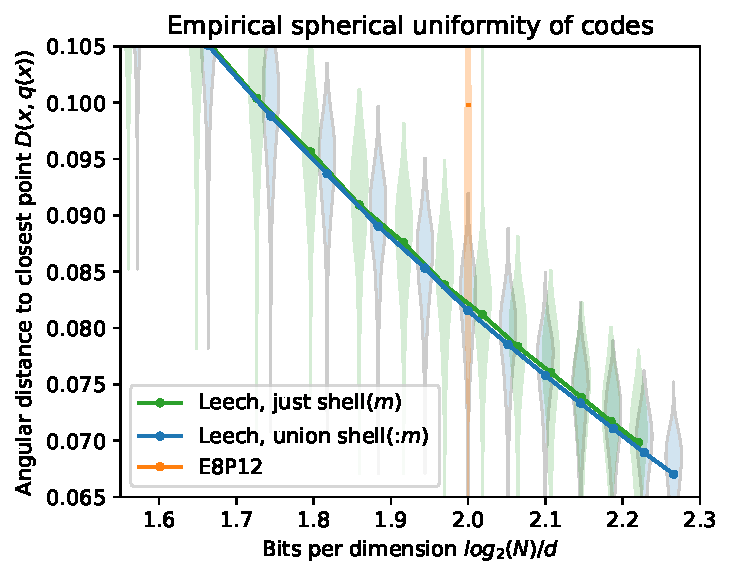
\includegraphics[]{figures/empirical-spherical-uniformity.pdf}
  }
  \caption{Empirical angular separation vs.\ rate. For each code, we show the distribution over nearest–neighbor angle against bits per dimension \(\log_2(N)/d\). The two Leech-based constructions are traced by varying \(m\) (single shell \(m\) vs.\ union \(1{:}m\)). We compare to E8P12 and find that it lies above the Leech curves at the same bits (worse angular separation), while between the Leech variants the union has slightly superior angular distance.}
  \label{fig:leech-shells-vs-union}
\end{figure}

We evaluate three code families as a function of bits: (1) Leech (single shell \(m\)), i.e., points from a single Leech shell projected to the unit sphere; (2) Leech (union up to \(m\)), i.e., the cumulative union of shells \(1{:}m\), all normalized to unit norm; and (3) the E8P12 product code for reference, normalized to the unit sphere and stacked three times to allow comparison in 24 dimensions. Figure~\ref{fig:leech-shells-vs-union} shows violin plots of the resulting distributions over \(D_{24}(x, q(x))\) versus bits for these three constructions. Empirically, we find that both Leech constructions, single shell \(m\) and union up to shell \(m\), perform similarly, with the union exhibiting slightly better code quality per bit as measured by angular uniformity.

Our empirical results indicate that \emph{using a union of shells (ball cut) of the Leech lattice yields a slightly better rate--distortion curve than using a single shell} on a Gaussian random source. We therefore adopt this approach in our method and recommend doing the same.

\newpage
\section{Spherical shaping or shape–gain: which achieves the lower distortion?}
\label{app:spherical-bounding-vs-shape-gain}

We consider two natural ways to construct a finite representation from a finite set of spherically bounded Leech lattice points (or from a single lattice shell), namely \emph{spherical shaping}, which uses the unnormalized points directly, and \emph{shape–gain}, which separates direction and magnitude via a projected spherical code for shape and a scalar gain code. Define \(C_{\text{spherical-shaping}} = \Lambda_{24}(m)\), the set of all lattice points in \(\Lambda_{24}\) whose squared norm is at most \(m\). We keep every lattice point inside a ball, and the resulting codebook directly inherits both its directions and its radii from the geometry of \(\Lambda_{24}\), up to a channel-wise or global scale. Intuitively, this is a very simple construction: one hyperparameter \(m\) determines both how far the code extends in radius and how many points it contains. The tradeoff between shape and gain is fixed implicitly by the lattice itself.

For shape–gain, we instead separate a vector into its magnitude and direction, \(x = r\,u\) with \(u = x/\|x\|\) and \(r=\|x\|\), and quantize these two pieces independently. Formally, define the shape code \(C_{\text{shape}} = \{\, x/\|x\| : x \in \Lambda_{24}(m)\,\}\), i.e., lattice points normalized to lie on the unit sphere, which gives a dense spherical code on \(S^{23}\). The gain is represented by a scalar gain code \(C_{\text{gain}}\) (e.g., matched to a \(\chi_{24}\) distribution for Gaussian sources). The full shape–gain code is then \(C_{\text{shape-gain}} = \{\, \hat r\, \hat u : \hat u \in C_{\text{shape}},\ \hat r \in C_{\text{gain}}\,\} = C_{\text{gain}} \times C_{\text{shape}}\). Intuitively, spherical shaping uses the raw lattice: you pick a lattice vector and both its direction and its length are “baked in.’’ In contrast, shape–gain forces every codeword direction to live on the sphere (from the projected lattice) and assigns its radius explicitly through the gain quantizer. In this sense, spherical shaping is geometric and monolithic, whereas shape–gain is modular and more flexible.

Because shape–gain has two components, it requires a choice of how to allocate bits between the direction (shape) part and the radius (gain) part. High-resolution theory provides a useful heuristic: in \(n\) dimensions, about \(1/n\) of the total bits should be devoted to gain, meaning that for \(n=24\) one should allocate roughly \(1/24\) of the rate to \(C_{\text{gain}}\) and the remainder to \(C_{\text{shape}}\). This gives a principled starting point and greatly reduces the effective search over hyperparameters. In contrast, the spherically bounded code \(C_{\text{spherically-bounded}} = \Lambda_{24}(m)\) has only one hyperparameter \(m\), which makes it easier to sweep but less expressive: it cannot optimize radius resolution independently of directional resolution.

We therefore compare these two constructions empirically under matched rate budgets: (i) the spherically bounded approach using \(C_{\text{spherically-bounded}} = \Lambda_{24}(m)\), and (ii) the shape–gain approach using \(C_{\text{shape-gain}} = C_{\text{gain}} \times C_{\text{shape}}\), where \(C_{\text{shape}} = \{x/\|x\| : x \in \Lambda_{24}(m)\}\) and \(C_{\text{gain}}\) is a \(\chi_{24}\)-matched scalar quantizer with approximately \(1/24\) of the available bits. This allows us to isolate the effect of separating radius and direction from the effect of simply using a spherically truncated lattice. 

\begin{table}[h]
    \centering
\resizebox{\linewidth}{!}{
    \begin{tabular}{l r c c | c c c}
       \textbf{Method} & \textbf{Code} &  & \textbf{Bits/dim} & \textbf{$\widehat{\text{MSE}}$} & \textbf{$\widehat{\text{SQNR}}$} (bits) & \textbf{Ret}(\%) \\
       \hline
       Leech (spherical bounding) & $\Lambda_{24}(13) $ & & 2.0 & 0.084 & 1.787 & 89.37 \\
       \hline
       Leech (shape-gain) & $\text{norm}(\Lambda_{24}(13))$ + 0 $\chi$-gain bits & 2.00000 + 0.00000 & 2.0 & 0.085 & 1.782 & 89.12 \\
       Leech (shape-gain) & $\text{norm}(\Lambda_{24}(12))$ + 1 $\chi$-gain bits & 1.95833 + 0.04167 & 2.0 & 0.078 & 1.843 & \textbf{92.14} \\
       Leech (shape-gain) & $\text{norm}(\Lambda_{24}(11))$ + 2 $\chi$-gain bits & 1.91667 + 0.08333 & 2.0 & 0.080 & 1.825 & 91.24 \\
       Leech (shape-gain) & $\text{norm}(\Lambda_{24}(10))$ + 4 $\chi$-gain bits & 1.83333 + 0.16667 & 2.0 & 0.085 & 1.780 & 89.01 \\
       \hline
    \end{tabular}
    }
    \caption{Comparison between spherical shaping and shape--gain quantization at a fixed budget of 2 bits/dim. For shape--gain we vary the allocation between directional (shape) bits and radial (gain) bits while keeping the total rate fixed.}
    \label{tab:spherical-bounding-vs-shape-gain}
\end{table}

It is evident from Table~\ref{tab:spherical-bounding-vs-shape-gain} that the shape--gain construction can outperform spherical shaping when evaluated on random Gaussian input at a fixed rate of 2 bits/dim. The best-performing configuration allocates one bit to the gain and the remainder to the shape code, achieving lower MSE and substantially higher retention. Notably, this optimal allocation (1 gain bit, or equivalently, 0.041 gain bits/dim) is close to, though slightly smaller than, what high-resolution theory would prescribe. Since in \(n\) dimensions approximately \(1/n\) of the bits should be assigned to gain, the heuristic for \(n=24\) would recommend using 2 gain bits (0.083 gain bits/dim), whereas our empirically optimal value is 1 gain bit in this case. The observed discrepancy is unsurprising: the theoretical allocation is derived in the asymptotic high-rate regime, whereas our experiments operate at a fixed, finite rate of 2 bits/dim. The empirical results indicate that (i) shape–gain coding improves performance over spherical shaping, (ii) the 1/24‑bit rule serves as a reasonable, though not necessarily optimal, heuristic for gain allocation, and (iii) for our Leech-based shape-gain code, we recommend 1 gain bits (0.041 gain bits/dim) or performing similar sweep at other bitrates for best possible quantization performance.


% \section{Literature review of downstream performance}
% 
% 
% \begin{table*}[t]
% \centering
% \caption{Comparison with wider set of methods for quantizing Llama-v3-8B model using different quantization methods, evaluated by wikitext-2 perplexity (PPL) and downstream task performance (CSR and MMLU). LLVQ consistently outperforms standard vector quantization approaches in performance against bits per parameter (Bits). *: assumed, not entirely clear from paper.}
% \hspace{0.8em}
% \label{tab:ptq-performance-literature}
% \resizebox{\linewidth}{!}{
% \begin{tabular}{l l r c | c || c | c c c c c c |}
% & & & & & \multicolumn{7}{c}{Llama-2 7B} \\
% \textbf{Method} & \textbf{Source} & \textbf{Finetuned} & \textbf{LM Eval} & \textbf{BPW} & \textbf{MMLU} & \textbf{Arc-C} & \textbf{Arc-E} & \textbf{BoolQ} & \textbf{Winogrande} & \textbf{Hellaswag} & \textbf{PiQA} \\
% \hline
% Baseline & (ours) & - & acc & 16 & 45.85 & 43.2 & 75.6 & 79.3 & 69.9 & 57.1 & 78.1  \\
% Baseline & Table 3 of Quip\# paper & & acc & 16 & & 40.6 & 69.3 & 78.5 & 67.3 & - & - \\
% Baseline & Table 10 of Quip\# paper & & acc & 16 & & - & - & 71.0 & 67.0 & - & \\
% Baseline & Table 10 of Quip\# paper & & acc\_norm & 16 & & 40.6 & 53.5 & - & - & - & 76.9\\
% Baseline & Table 6 of QTIP paper & & acc? & 16 & & 40.0 & 69.3 & - & 67.3 & - & 78.5 \\
% Baseline & Table 8 of PV-tuning paper & & acc & 16 & & 43.4 & 76.3 & - & 69.1 & 57.1 & 78.1 \\
% Baseline & Table 10 of GPTVQ paper & & acc & 16 & & 46.3 & 74.6 & 77.7 & 69.1 & 76.0 & 79.1 \\
% \hline
% Quip\# & Table 10 of Quip\# paper & no finetuning & acc & 2 & & & - & 62.3 & 62.4 & - & - \\
% Quip\# & Table 10 of Quip\# paper & no finetuning & acc\_norm & 2 & & 32.5 & 42.8 & - & - & - & 71.2 \\
% \hline
% %GPTVQ & Table 10 of GPTQ paper & not reported & ? & 2.125 & - & 34.4 & 60.4 & 65.5 & 65.0 & (64.0) & 73.3 \\
% %\hline
% LLVQ (spherical shaping) & (\textbf{ours}) & no finetuning & acc & 2 & [j, 
% colorful-rain] \\
% LLVQ (shape-gain chi) & (\textbf{ours}) & no finetuning & acc & 2 & [0, skilled-sponge] \\
% \hline
% \hline
% Quip &  Table 3 of Quip\# paper & Yes* & acc & 2 & & 19.4 & 26.0 & 54.6 & 51.8 & - & - \\
% OmniQ & Table 3 of Quip\# paper & Yes* & acc & 2 & & 21.6 & 35.2 & 57.5 & 51.5 & - & - \\
% AQLM &  Table 3 of Quip\# paper & Yes & acc & 2.07 & & 33.6 & 62.8 & 73.5 & 64.6 & - & - \\
% Quip\# & Table 3 of Quip\# paper & Yes* & acc & 2 & & 34.6 & 64.6 & 75.1 & 64.9 & - & - \\
% Quip\# & Table 10 of Quip\# paper & Yes & acc & 2 & & - & - & 68.3 & 64.9 & - & - \\
% Quip\# & Table 10 of Quip\# paper & Yes & acc\_norm & 2 & & 36.1 & 50.5 & - & - & - & 74.9 \\
% AQLM & Table 6 of QTIP paper & Yes & acc? & 2.07 & & 32.8 & 63.7 & 74.8 & 65.7 & - & - \\
% Quip\# & Table 6 of QTIP paper & Yes & acc? & 2 & & 35.2 & 65.3 & 75.4 & 64.9 & - & - \\
% QTIP & Table 6 of QTIP paper & Yes & acc? & 2 & & 35.7 & 65.6 & 75.9 & 64.7 & - & - \\
% PV-tuning & Table 8 of PV-tuning paper & Yes & acc & 2 & & 38.4 & 71.17 & - & 66.7 & 53.5 & 77.0 \\
% \hline
% LLVQ (spherical shaping) & (\textbf{ours}) & Yes & acc & 2 & [j, 
% colorful-rain] \\
% LLVQ (shape-gain chi) & (\textbf{ours}) & Yes & acc & 2 & [0, skilled-sponge] \\
% \hline
% \end{tabular}
% \vspace{-1em}
% }
% \end{table*}



% \section{Overview of vectors in each shell}
% 
% Table~\ref{tab:leech-shell-example} summarizes the distribution of vectors across shells of the Leech lattice, grouped by parity and indexed by shell number \(m\). For each shell, we report the total count of vectors and the frequency of coordinates.
% 
% It can be noted that shells grow rapidly in size as \(m\) increases, with counts ranging from thousands to hundreds of millions. Shells with large counts result in spherical codes with higher rates, while the distribution of the values affects angular uniformity when projecting to the unit sphere.
% 
% \subsection{Shells $m=2$ up to $m=6$}
% 
% \begin{table}[h!]
% \centering
% \setlength{\tabcolsep}{3pt}
% \renewcommand{\arraystretch}{0.9}
% %\resizebox{0.4\linewidth}{!}{
% \begin{tabular}{c c r | c c c c c c c c}
% m & parity & count & $\pm$7 & $\pm$6 & $\pm$5 & $\pm$4 & $\pm$3 & $\pm$2 & $\pm$1 & $\pm$0 \\
% \hline
% 2 & even & 1104 & 0 & 0 & 0 & 2 & 0 & 0 & 0 & 22 \\
%  & even & 97152 & 0 & 0 & 0 & 0 & 0 & 8 & 0 & 16 \\
% \cdashline{4-11}[5pt/4pt]
%  & odd & 98304 & 0 & 0 & 0 & 0 & 1 & 0 & 23 & 0 \\
% \hline
% 3 & even & 3108864 & 0 & 0 & 0 & 1 & 0 & 8 & 0 & 15 \\
%  & even & 5275648 & 0 & 0 & 0 & 0 & 0 & 12 & 0 & 12 \\
% \cdashline{4-11}[5pt/4pt]
%  & odd & 98304 & 0 & 0 & 1 & 0 & 0 & 0 & 23 & 0 \\
%  & odd & 8290304 & 0 & 0 & 0 & 0 & 3 & 0 & 21 & 0 \\
% \hline
% 4 & even & 170016 & 0 & 0 & 0 & 4 & 0 & 0 & 0 & 20 \\
%  & even & 48 & 0 & 0 & 0 & 0 & 0 & 0 & 0 & 23 \\
%  & even & 46632960 & 0 & 0 & 0 & 2 & 0 & 8 & 0 & 14 \\
%  & even & 777216 & 0 & 1 & 0 & 0 & 0 & 7 & 0 & 16 \\
%  & even & 126615552 & 0 & 0 & 0 & 1 & 0 & 12 & 0 & 11 \\
%  & even & 24870912 & 0 & 0 & 0 & 0 & 0 & 16 & 0 & 8 \\
% \cdashline{4-11}[5pt/4pt]
%  & odd & 24870912 & 0 & 0 & 1 & 0 & 2 & 0 & 21 & 0 \\
%  & odd & 174096384 & 0 & 0 & 0 & 0 & 5 & 0 & 19 & 0 \\
% \hline
% 5 & even & 435240960 & 0 & 0 & 0 & 3 & 0 & 8 & 0 & 13 \\
%  & even & 24870912 & 0 & 1 & 0 & 1 & 0 & 7 & 0 & 15 \\
%  & even & 1392771072 & 0 & 0 & 0 & 2 & 0 & 12 & 0 & 10 \\
%  & even & 63307776 & 0 & 1 & 0 & 0 & 0 & 11 & 0 & 12 \\
%  & even & 397934592 & 0 & 0 & 0 & 1 & 0 & 16 & 0 & 7 \\
% \cdashline{4-11}[5pt/4pt]
%  & odd & 2260992 & 1 & 0 & 0 & 0 & 1 & 0 & 22 & 0 \\
%  & odd & 24870912 & 0 & 0 & 2 & 0 & 1 & 0 & 21 & 0 \\
%  & odd & 870481920 & 0 & 0 & 1 & 0 & 4 & 0 & 19 & 0 \\
%  & odd & 1417641984 & 0 & 0 & 0 & 0 & 7 & 0 & 17 & 0 \\
% \hline
% 6 & even & 8614144 & 0 & 0 & 0 & 6 & 0 & 0 & 0 & 18 \\
%  & even & 48576 & 0 & 0 & 0 & 2 & 0 & 0 & 0 & 21 \\
%  & even & 2829066240 & 0 & 0 & 0 & 4 & 0 & 8 & 0 & 12 \\
%  & even & 373063680 & 0 & 1 & 0 & 2 & 0 & 7 & 0 & 14 \\
%  & even & 2720256 & 0 & 2 & 0 & 0 & 0 & 6 & 0 & 16 \\
%  & even & 3108864 & 0 & 0 & 0 & 0 & 0 & 8 & 0 & 15 \\
%  & even & 9285140480 & 0 & 0 & 0 & 3 & 0 & 12 & 0 & 9 \\
%  & even & 1519386624 & 0 & 1 & 0 & 1 & 0 & 11 & 0 & 11 \\
%  & even & 2785542144 & 0 & 0 & 0 & 2 & 0 & 16 & 0 & 6 \\
%  & even & 397934592 & 0 & 1 & 0 & 0 & 0 & 15 & 0 & 8 \\
%  & even & 8388608 & 0 & 0 & 0 & 0 & 0 & 24 & 0 & 0 \\
% \cdashline{4-11}[5pt/4pt]
%  & odd & 2260992 & 1 & 0 & 1 & 0 & 0 & 0 & 22 & 0 \\
%  & odd & 174096384 & 1 & 0 & 0 & 0 & 3 & 0 & 20 & 0 \\
%  & odd & 8290304 & 0 & 0 & 3 & 0 & 0 & 0 & 21 & 0 \\
%  & odd & 1740963840 & 0 & 0 & 2 & 0 & 3 & 0 & 19 & 0 \\
%  & odd & 9923493888 & 0 & 0 & 1 & 0 & 6 & 0 & 17 & 0 \\
%  & odd & 5355536384 & 0 & 0 & 0 & 0 & 9 & 0 & 15 & 0 \\
% \end{tabular}
% %}
% \caption{Example counts per shell $m$ in Leech lattice.}
% \label{tab:leech-shell-example}
% \end{table}
% 
% \newpage
% \subsection{Shells $m=7$ and $m=8$}
% 
% \begin{table}[h!]
% \centering
% \setlength{\tabcolsep}{3pt}
% \renewcommand{\arraystretch}{0.9}
% \resizebox{0.6\linewidth}{!}{
% \begin{tabular}{c c r | c c c c c c c c c c}
% m & parity & count & $\pm$9 & $\pm$8 & $\pm$7 & $\pm$6 & $\pm$5 & $\pm$4 & $\pm$3 & $\pm$2 & $\pm$1 & $\pm$0 \\
% \hline
% 7 & even & 13579517952 & 0 & 0 & 0 & 0 & 0 & 5 & 0 & 8 & 0 & 11 \\
%  & even & 3481927680 & 0 & 0 & 0 & 1 & 0 & 3 & 0 & 7 & 0 & 13 \\
%  & even & 87048192 & 0 & 0 & 0 & 2 & 0 & 1 & 0 & 6 & 0 & 15 \\
%  & even & 93265920 & 0 & 1 & 0 & 0 & 0 & 1 & 0 & 8 & 0 & 14 \\
%  & even & 41783132160 & 0 & 0 & 0 & 0 & 0 & 4 & 0 & 12 & 0 & 8 \\
%  & even & 16713252864 & 0 & 0 & 0 & 1 & 0 & 2 & 0 & 11 & 0 & 10 \\
%  & even & 348192768 & 0 & 0 & 0 & 2 & 0 & 0 & 0 & 10 & 0 & 12 \\
%  & even & 126615552 & 0 & 1 & 0 & 0 & 0 & 0 & 0 & 12 & 0 & 11 \\
%  & even & 11142168576 & 0 & 0 & 0 & 0 & 0 & 3 & 0 & 16 & 0 & 5 \\
%  & even & 6366953472 & 0 & 0 & 0 & 1 & 0 & 1 & 0 & 15 & 0 & 7 \\
% \cdashline{4-11}[5pt/4pt]
%  & odd & 2260992 & 1 & 0 & 0 & 0 & 0 & 0 & 1 & 0 & 22 & 0 \\
%  & odd & 522289152 & 0 & 0 & 1 & 0 & 1 & 0 & 2 & 0 & 20 & 0 \\
%  & odd & 3307831296 & 0 & 0 & 1 & 0 & 0 & 0 & 5 & 0 & 18 & 0 \\
%  & odd & 1740963840 & 0 & 0 & 0 & 0 & 3 & 0 & 2 & 0 & 19 & 0 \\
%  & odd & 29770481664 & 0 & 0 & 0 & 0 & 2 & 0 & 5 & 0 & 17 & 0 \\
%  & odd & 48199827456 & 0 & 0 & 0 & 0 & 1 & 0 & 8 & 0 & 15 & 0 \\
%  & odd & 10224205824 & 0 & 0 & 0 & 0 & 0 & 0 & 11 & 0 & 13 & 0 \\
% \hline
% 8 & even & 188280576 & 0 & 0 & 0 & 0 & 0 & 8 & 0 & 0 & 0 & 16 \\
%  & even & 6800640 & 0 & 1 & 0 & 0 & 0 & 4 & 0 & 0 & 0 & 19 \\
%  & even & 1104 & 0 & 2 & 0 & 0 & 0 & 0 & 0 & 0 & 0 & 22 \\
%  & even & 49791565824 & 0 & 0 & 0 & 0 & 0 & 6 & 0 & 8 & 0 & 10 \\
%  & even & 22632529920 & 0 & 0 & 0 & 1 & 0 & 4 & 0 & 7 & 0 & 12 \\
%  & even & 1305722880 & 0 & 0 & 0 & 2 & 0 & 2 & 0 & 6 & 0 & 14 \\
%  & even & 5440512 & 0 & 0 & 0 & 3 & 0 & 0 & 0 & 5 & 0 & 16 \\
%  & even & 1305722880 & 0 & 1 & 0 & 0 & 0 & 2 & 0 & 8 & 0 & 13 \\
%  & even & 24870912 & 0 & 1 & 0 & 1 & 0 & 0 & 0 & 7 & 0 & 15 \\
%  & even & 777216 & 0 & 0 & 0 & 0 & 0 & 0 & 0 & 7 & 0 & 16 \\
%  & even & 133706022912 & 0 & 0 & 0 & 0 & 0 & 5 & 0 & 12 & 0 & 7 \\
%  & even & 111421685760 & 0 & 0 & 0 & 1 & 0 & 3 & 0 & 11 & 0 & 9 \\
%  & even & 8356626432 & 0 & 0 & 0 & 2 & 0 & 1 & 0 & 10 & 0 & 11 \\
%  & even & 2785542144 & 0 & 1 & 0 & 0 & 0 & 1 & 0 & 12 & 0 & 10 \\
%  & even & 27855421440 & 0 & 0 & 0 & 0 & 0 & 4 & 0 & 16 & 0 & 4 \\
%  & even & 44568674304 & 0 & 0 & 0 & 1 & 0 & 2 & 0 & 15 & 0 & 6 \\
%  & even & 2984509440 & 0 & 0 & 0 & 2 & 0 & 0 & 0 & 14 & 0 & 8 \\
%  & even & 397934592 & 0 & 1 & 0 & 0 & 0 & 0 & 0 & 16 & 0 & 7 \\
%  & even & 201326592 & 0 & 0 & 0 & 1 & 0 & 0 & 0 & 23 & 0 & 0 \\
% \cdashline{4-11}[5pt/4pt]
%  & odd & 2260992 & 1 & 0 & 0 & 0 & 1 & 0 & 0 & 0 & 22 & 0 \\
%  & odd & 174096384 & 1 & 0 & 0 & 0 & 0 & 0 & 3 & 0 & 20 & 0 \\
%  & odd & 24870912 & 0 & 0 & 2 & 0 & 0 & 0 & 1 & 0 & 21 & 0 \\
%  & odd & 522289152 & 0 & 0 & 1 & 0 & 2 & 0 & 1 & 0 & 20 & 0 \\
%  & odd & 16539156480 & 0 & 0 & 1 & 0 & 1 & 0 & 4 & 0 & 18 & 0 \\
%  & odd & 24099913728 & 0 & 0 & 1 & 0 & 0 & 0 & 7 & 0 & 16 & 0 \\
%  & odd & 870481920 & 0 & 0 & 0 & 0 & 4 & 0 & 1 & 0 & 19 & 0 \\
%  & odd & 49617469440 & 0 & 0 & 0 & 0 & 3 & 0 & 4 & 0 & 17 & 0 \\
%  & odd & 192799309824 & 0 & 0 & 0 & 0 & 2 & 0 & 7 & 0 & 15 & 0 \\
%  & odd & 112466264064 & 0 & 0 & 0 & 0 & 1 & 0 & 10 & 0 & 13 & 0 \\
%  & odd & 10224205824 & 0 & 0 & 0 & 0 & 0 & 0 & 13 & 0 & 11 & 0 \\
% \end{tabular}
% }
% \caption{Example counts per shell $m$ in Leech lattice.}
% \label{tab:leech-shell-example-2}
% \end{table}
% 
% \newpage
% \subsection{Shells $m=9$ and $m=10$}
% 
% \begin{table}[h!]
% \centering
% \setlength{\tabcolsep}{3pt}
% \renewcommand{\arraystretch}{0.9}
% \resizebox{0.4\linewidth}{!}{
% 
% \begin{tabular}{c c r | c c c c c c c c c c c c}
% m & parity & count & $\pm$11 & $\pm$10 & $\pm$9 & $\pm$8 & $\pm$7 & $\pm$6 & $\pm$5 & $\pm$4 & $\pm$3 & $\pm$2 & $\pm$1 & $\pm$0 \\
% \hline
% 9 & even & 142261616640 & 0 & 0 & 0 & 0 & 0 & 0 & 0 & 7 & 0 & 8 & 0 & 9 \\
%  & even & 108636143616 & 0 & 0 & 0 & 0 & 0 & 1 & 0 & 5 & 0 & 7 & 0 & 11 \\
%  & even & 12186746880 & 0 & 0 & 0 & 0 & 0 & 2 & 0 & 3 & 0 & 6 & 0 & 13 \\
%  & even & 174096384 & 0 & 0 & 0 & 0 & 0 & 3 & 0 & 1 & 0 & 5 & 0 & 15 \\
%  & even & 11316264960 & 0 & 0 & 0 & 1 & 0 & 0 & 0 & 3 & 0 & 8 & 0 & 12 \\
%  & even & 746127360 & 0 & 0 & 0 & 1 & 0 & 1 & 0 & 1 & 0 & 7 & 0 & 14 \\
%  & even & 24870912 & 0 & 1 & 0 & 0 & 0 & 0 & 0 & 1 & 0 & 7 & 0 & 15 \\
%  & even & 311980720128 & 0 & 0 & 0 & 0 & 0 & 0 & 0 & 6 & 0 & 12 & 0 & 6 \\
%  & even & 501397585920 & 0 & 0 & 0 & 0 & 0 & 1 & 0 & 4 & 0 & 11 & 0 & 8 \\
%  & even & 91922890752 & 0 & 0 & 0 & 0 & 0 & 2 & 0 & 2 & 0 & 10 & 0 & 10 \\
%  & even & 1160642560 & 0 & 0 & 0 & 0 & 0 & 3 & 0 & 0 & 0 & 9 & 0 & 12 \\
%  & even & 27855421440 & 0 & 0 & 0 & 1 & 0 & 0 & 0 & 2 & 0 & 12 & 0 & 9 \\
%  & even & 1519386624 & 0 & 0 & 0 & 1 & 0 & 1 & 0 & 0 & 0 & 11 & 0 & 11 \\
%  & even & 63307776 & 0 & 1 & 0 & 0 & 0 & 0 & 0 & 0 & 0 & 11 & 0 & 12 \\
%  & even & 44568674304 & 0 & 0 & 0 & 0 & 0 & 0 & 0 & 5 & 0 & 16 & 0 & 3 \\
%  & even & 178274697216 & 0 & 0 & 0 & 0 & 0 & 1 & 0 & 3 & 0 & 15 & 0 & 5 \\
%  & even & 47752151040 & 0 & 0 & 0 & 0 & 0 & 2 & 0 & 1 & 0 & 14 & 0 & 7 \\
%  & even & 5571084288 & 0 & 0 & 0 & 1 & 0 & 0 & 0 & 1 & 0 & 16 & 0 & 6 \\
% \cdashline{4-11}[5pt/4pt]
%  & odd & 98304 & 1 & 0 & 0 & 0 & 0 & 0 & 0 & 0 & 0 & 0 & 23 & 0 \\
%  & odd & 522289152 & 0 & 0 & 1 & 0 & 0 & 0 & 1 & 0 & 2 & 0 & 20 & 0 \\
%  & odd & 3307831296 & 0 & 0 & 1 & 0 & 0 & 0 & 0 & 0 & 5 & 0 & 18 & 0 \\
%  & odd & 24870912 & 0 & 0 & 0 & 0 & 2 & 0 & 1 & 0 & 0 & 0 & 21 & 0 \\
%  & odd & 1740963840 & 0 & 0 & 0 & 0 & 2 & 0 & 0 & 0 & 3 & 0 & 19 & 0 \\
%  & odd & 174096384 & 0 & 0 & 0 & 0 & 1 & 0 & 3 & 0 & 0 & 0 & 20 & 0 \\
%  & odd & 33078312960 & 0 & 0 & 0 & 0 & 1 & 0 & 2 & 0 & 3 & 0 & 18 & 0 \\
%  & odd & 168699396096 & 0 & 0 & 0 & 0 & 1 & 0 & 1 & 0 & 6 & 0 & 16 & 0 \\
%  & odd & 80333045760 & 0 & 0 & 0 & 0 & 1 & 0 & 0 & 0 & 9 & 0 & 14 & 0 \\
%  & odd & 174096384 & 0 & 0 & 0 & 0 & 0 & 0 & 5 & 0 & 0 & 0 & 19 & 0 \\
%  & odd & 49617469440 & 0 & 0 & 0 & 0 & 0 & 0 & 4 & 0 & 3 & 0 & 17 & 0 \\
%  & odd & 449865056256 & 0 & 0 & 0 & 0 & 0 & 0 & 3 & 0 & 6 & 0 & 15 & 0 \\
%  & odd & 562331320320 & 0 & 0 & 0 & 0 & 0 & 0 & 2 & 0 & 9 & 0 & 13 & 0 \\
%  & odd & 132914675712 & 0 & 0 & 0 & 0 & 0 & 0 & 1 & 0 & 12 & 0 & 11 & 0 \\
%  & odd & 5355536384 & 0 & 0 & 0 & 0 & 0 & 0 & 0 & 0 & 15 & 0 & 9 & 0 \\
% \hline
% 10 & even & 2008326144 & 0 & 0 & 0 & 0 & 0 & 0 & 0 & 10 & 0 & 0 & 0 & 14 \\
%  & even & 310109184 & 0 & 0 & 0 & 1 & 0 & 0 & 0 & 6 & 0 & 0 & 0 & 17 \\
%  & even & 1020096 & 0 & 0 & 0 & 2 & 0 & 0 & 0 & 2 & 0 & 0 & 0 & 20 \\
%  & even & 2208 & 0 & 0 & 0 & 0 & 0 & 0 & 0 & 1 & 0 & 0 & 0 & 22 \\
%  & even & 320088637440 & 0 & 0 & 0 & 0 & 0 & 0 & 0 & 8 & 0 & 8 & 0 & 8 \\
%  & even & 398332526592 & 0 & 0 & 0 & 0 & 0 & 1 & 0 & 6 & 0 & 7 & 0 & 10 \\
%  & even & 79213854720 & 0 & 0 & 0 & 0 & 0 & 2 & 0 & 4 & 0 & 6 & 0 & 12 \\
%  & even & 2611445760 & 0 & 0 & 0 & 0 & 0 & 3 & 0 & 2 & 0 & 5 & 0 & 14 \\
%  & even & 6800640 & 0 & 0 & 0 & 0 & 0 & 4 & 0 & 0 & 0 & 4 & 0 & 16 \\
%  & even & 67897589760 & 0 & 0 & 0 & 1 & 0 & 0 & 0 & 4 & 0 & 8 & 0 & 11 \\
%  & even & 10445783040 & 0 & 0 & 0 & 1 & 0 & 1 & 0 & 2 & 0 & 7 & 0 & 13 \\
%  & even & 87048192 & 0 & 0 & 0 & 1 & 0 & 2 & 0 & 0 & 0 & 6 & 0 & 15 \\
%  & even & 46632960 & 0 & 0 & 0 & 2 & 0 & 0 & 0 & 0 & 0 & 8 & 0 & 14 \\
%  & even & 373063680 & 0 & 1 & 0 & 0 & 0 & 0 & 0 & 2 & 0 & 7 & 0 & 14 \\
%  & even & 5440512 & 0 & 1 & 0 & 0 & 0 & 1 & 0 & 0 & 0 & 6 & 0 & 16 \\
%  & even & 534824091648 & 0 & 0 & 0 & 0 & 0 & 0 & 0 & 7 & 0 & 12 & 0 & 5 \\
%  & even & 1604472274944 & 0 & 0 & 0 & 0 & 0 & 1 & 0 & 5 & 0 & 11 & 0 & 7 \\
%  & even & 612819271680 & 0 & 0 & 0 & 0 & 0 & 2 & 0 & 3 & 0 & 10 & 0 & 9 \\
%  & even & 27855421440 & 0 & 0 & 0 & 0 & 0 & 3 & 0 & 1 & 0 & 9 & 0 & 11 \\
%  & even & 167132528640 & 0 & 0 & 0 & 1 & 0 & 0 & 0 & 3 & 0 & 12 & 0 & 8 \\
%  & even & 33426505728 & 0 & 0 & 0 & 1 & 0 & 1 & 0 & 1 & 0 & 11 & 0 & 10 \\
%  & even & 1519386624 & 0 & 1 & 0 & 0 & 0 & 0 & 0 & 1 & 0 & 11 & 0 & 11 \\
%  & even & 44568674304 & 0 & 0 & 0 & 0 & 0 & 0 & 0 & 6 & 0 & 16 & 0 & 2 \\
%  & even & 445686743040 & 0 & 0 & 0 & 0 & 0 & 1 & 0 & 4 & 0 & 15 & 0 & 4 \\
%  & even & 334265057280 & 0 & 0 & 0 & 0 & 0 & 2 & 0 & 2 & 0 & 14 & 0 & 6 \\
%  & even & 13927710720 & 0 & 0 & 0 & 0 & 0 & 3 & 0 & 0 & 0 & 13 & 0 & 8 \\
%  & even & 33426505728 & 0 & 0 & 0 & 1 & 0 & 0 & 0 & 2 & 0 & 16 & 0 & 5 \\
%  & even & 6366953472 & 0 & 0 & 0 & 1 & 0 & 1 & 0 & 0 & 0 & 15 & 0 & 7 \\
%  & even & 397934592 & 0 & 1 & 0 & 0 & 0 & 0 & 0 & 0 & 0 & 15 & 0 & 8 \\
%  & even & 2315255808 & 0 & 0 & 0 & 0 & 0 & 2 & 0 & 0 & 0 & 22 & 0 & 0 \\
% \cdashline{4-11}[5pt/4pt]
%  & odd & 24870912 & 1 & 0 & 0 & 0 & 0 & 0 & 0 & 0 & 2 & 0 & 21 & 0 \\
%  & odd & 49741824 & 0 & 0 & 1 & 0 & 1 & 0 & 0 & 0 & 1 & 0 & 21 & 0 \\
%  & odd & 522289152 & 0 & 0 & 1 & 0 & 0 & 0 & 2 & 0 & 1 & 0 & 20 & 0 \\
%  & odd & 16539156480 & 0 & 0 & 1 & 0 & 0 & 0 & 1 & 0 & 4 & 0 & 18 & 0 \\
%  & odd & 24099913728 & 0 & 0 & 1 & 0 & 0 & 0 & 0 & 0 & 7 & 0 & 16 & 0 \\
%  & odd & 5222891520 & 0 & 0 & 0 & 0 & 2 & 0 & 1 & 0 & 2 & 0 & 19 & 0 \\
%  & odd & 29770481664 & 0 & 0 & 0 & 0 & 2 & 0 & 0 & 0 & 5 & 0 & 17 & 0 \\
%  & odd & 33078312960 & 0 & 0 & 0 & 0 & 1 & 0 & 3 & 0 & 2 & 0 & 18 & 0 \\
%  & odd & 506098188288 & 0 & 0 & 0 & 0 & 1 & 0 & 2 & 0 & 5 & 0 & 16 & 0 \\
%  & odd & 722997411840 & 0 & 0 & 0 & 0 & 1 & 0 & 1 & 0 & 8 & 0 & 14 & 0 \\
%  & odd & 132914675712 & 0 & 0 & 0 & 0 & 1 & 0 & 0 & 0 & 11 & 0 & 12 & 0 \\
%  & odd & 29770481664 & 0 & 0 & 0 & 0 & 0 & 0 & 5 & 0 & 2 & 0 & 17 & 0 \\
%  & odd & 674797584384 & 0 & 0 & 0 & 0 & 0 & 0 & 4 & 0 & 5 & 0 & 15 & 0 \\
%  & odd & 1686993960960 & 0 & 0 & 0 & 0 & 0 & 0 & 3 & 0 & 8 & 0 & 13 & 0 \\
%  & odd & 797488054272 & 0 & 0 & 0 & 0 & 0 & 0 & 2 & 0 & 11 & 0 & 11 & 0 \\
%  & odd & 80333045760 & 0 & 0 & 0 & 0 & 0 & 0 & 1 & 0 & 14 & 0 & 9 & 0 \\
%  & odd & 1417641984 & 0 & 0 & 0 & 0 & 0 & 0 & 0 & 0 & 17 & 0 & 7 & 0 \\
% \end{tabular}
% }
% \caption{Example counts per shell $m$ in Leech lattice.}
% \label{tab:leech-shell-example-2}
% \end{table}
% 
% \newpage
% \subsection{Shells $m=11$ and $m=12$}
% 
% \begin{table}[h!]
% \centering
% \setlength{\tabcolsep}{3pt}
% \renewcommand{\arraystretch}{0.9}
% \resizebox{0.3\linewidth}{!}{
% \begin{tabular}{c c r | c c c c c c c c c c c c c}
% m & parity & count & $\pm$12 & $\pm$11 & $\pm$10 & $\pm$9 & $\pm$8 & $\pm$7 & $\pm$6 & $\pm$5 & $\pm$4 & $\pm$3 & $\pm$2 & $\pm$1 & $\pm$0 \\
% \hline
% 11 & even & 569046466560 & 0 & 0 & 0 & 0 & 0 & 0 & 0 & 0 & 9 & 0 & 8 & 0 & 7 \\
%  & even & 1138092933120 & 0 & 0 & 0 & 0 & 0 & 0 & 1 & 0 & 7 & 0 & 7 & 0 & 9 \\
%  & even & 380226502656 & 0 & 0 & 0 & 0 & 0 & 0 & 2 & 0 & 5 & 0 & 6 & 0 & 11 \\
%  & even & 24373493760 & 0 & 0 & 0 & 0 & 0 & 0 & 3 & 0 & 3 & 0 & 5 & 0 & 13 \\
%  & even & 217620480 & 0 & 0 & 0 & 0 & 0 & 0 & 4 & 0 & 1 & 0 & 4 & 0 & 15 \\
%  & even & 298749394944 & 0 & 0 & 0 & 0 & 1 & 0 & 0 & 0 & 5 & 0 & 8 & 0 & 10 \\
%  & even & 90530119680 & 0 & 0 & 0 & 0 & 1 & 0 & 1 & 0 & 3 & 0 & 7 & 0 & 12 \\
%  & even & 2611445760 & 0 & 0 & 0 & 0 & 1 & 0 & 2 & 0 & 1 & 0 & 6 & 0 & 14 \\
%  & even & 1305722880 & 0 & 0 & 0 & 0 & 2 & 0 & 0 & 0 & 1 & 0 & 8 & 0 & 13 \\
%  & even & 3481927680 & 0 & 0 & 1 & 0 & 0 & 0 & 0 & 0 & 3 & 0 & 7 & 0 & 13 \\
%  & even & 174096384 & 0 & 0 & 1 & 0 & 0 & 0 & 1 & 0 & 1 & 0 & 6 & 0 & 15 \\
%  & even & 3108864 & 1 & 0 & 0 & 0 & 0 & 0 & 0 & 0 & 0 & 0 & 8 & 0 & 15 \\
%  & even & 668530114560 & 0 & 0 & 0 & 0 & 0 & 0 & 0 & 0 & 8 & 0 & 12 & 0 & 4 \\
%  & even & 3743768641536 & 0 & 0 & 0 & 0 & 0 & 0 & 1 & 0 & 6 & 0 & 11 & 0 & 6 \\
%  & even & 2757686722560 & 0 & 0 & 0 & 0 & 0 & 0 & 2 & 0 & 4 & 0 & 10 & 0 & 8 \\
%  & even & 306409635840 & 0 & 0 & 0 & 0 & 0 & 0 & 3 & 0 & 2 & 0 & 9 & 0 & 10 \\
%  & even & 2611445760 & 0 & 0 & 0 & 0 & 0 & 0 & 4 & 0 & 0 & 0 & 8 & 0 & 12 \\
%  & even & 668530114560 & 0 & 0 & 0 & 0 & 1 & 0 & 0 & 0 & 4 & 0 & 12 & 0 & 7 \\
%  & even & 334265057280 & 0 & 0 & 0 & 0 & 1 & 0 & 1 & 0 & 2 & 0 & 11 & 0 & 9 \\
%  & even & 8356626432 & 0 & 0 & 0 & 0 & 1 & 0 & 2 & 0 & 0 & 0 & 10 & 0 & 11 \\
%  & even & 1392771072 & 0 & 0 & 0 & 0 & 2 & 0 & 0 & 0 & 0 & 0 & 12 & 0 & 10 \\
%  & even & 16713252864 & 0 & 0 & 1 & 0 & 0 & 0 & 0 & 0 & 2 & 0 & 11 & 0 & 10 \\
%  & even & 696385536 & 0 & 0 & 1 & 0 & 0 & 0 & 1 & 0 & 0 & 0 & 10 & 0 & 12 \\
%  & even & 25467813888 & 0 & 0 & 0 & 0 & 0 & 0 & 0 & 0 & 7 & 0 & 16 & 0 & 1 \\
%  & even & 713098788864 & 0 & 0 & 0 & 0 & 0 & 0 & 1 & 0 & 5 & 0 & 15 & 0 & 3 \\
%  & even & 1337060229120 & 0 & 0 & 0 & 0 & 0 & 0 & 2 & 0 & 3 & 0 & 14 & 0 & 5 \\
%  & even & 222843371520 & 0 & 0 & 0 & 0 & 0 & 0 & 3 & 0 & 1 & 0 & 13 & 0 & 7 \\
%  & even & 111421685760 & 0 & 0 & 0 & 0 & 1 & 0 & 0 & 0 & 3 & 0 & 16 & 0 & 4 \\
%  & even & 89137348608 & 0 & 0 & 0 & 0 & 1 & 0 & 1 & 0 & 1 & 0 & 15 & 0 & 6 \\
%  & even & 6366953472 & 0 & 0 & 1 & 0 & 0 & 0 & 0 & 0 & 1 & 0 & 15 & 0 & 7 \\
% \cdashline{4-11}[5pt/4pt]
%  & odd & 49741824 & 0 & 1 & 0 & 0 & 0 & 0 & 0 & 1 & 0 & 1 & 0 & 21 & 0 \\
%  & odd & 870481920 & 0 & 1 & 0 & 0 & 0 & 0 & 0 & 0 & 0 & 4 & 0 & 19 & 0 \\
%  & odd & 49741824 & 0 & 0 & 0 & 1 & 0 & 1 & 0 & 1 & 0 & 0 & 0 & 21 & 0 \\
%  & odd & 3481927680 & 0 & 0 & 0 & 1 & 0 & 1 & 0 & 0 & 0 & 3 & 0 & 19 & 0 \\
%  & odd & 174096384 & 0 & 0 & 0 & 1 & 0 & 0 & 0 & 3 & 0 & 0 & 0 & 20 & 0 \\
%  & odd & 33078312960 & 0 & 0 & 0 & 1 & 0 & 0 & 0 & 2 & 0 & 3 & 0 & 18 & 0 \\
%  & odd & 168699396096 & 0 & 0 & 0 & 1 & 0 & 0 & 0 & 1 & 0 & 6 & 0 & 16 & 0 \\
%  & odd & 80333045760 & 0 & 0 & 0 & 1 & 0 & 0 & 0 & 0 & 0 & 9 & 0 & 14 & 0 \\
%  & odd & 174096384 & 0 & 0 & 0 & 0 & 0 & 3 & 0 & 0 & 0 & 1 & 0 & 20 & 0 \\
%  & odd & 5222891520 & 0 & 0 & 0 & 0 & 0 & 2 & 0 & 2 & 0 & 1 & 0 & 19 & 0 \\
%  & odd & 148852408320 & 0 & 0 & 0 & 0 & 0 & 2 & 0 & 1 & 0 & 4 & 0 & 17 & 0 \\
%  & odd & 192799309824 & 0 & 0 & 0 & 0 & 0 & 2 & 0 & 0 & 0 & 7 & 0 & 15 & 0 \\
%  & odd & 16539156480 & 0 & 0 & 0 & 0 & 0 & 1 & 0 & 4 & 0 & 1 & 0 & 18 & 0 \\
%  & odd & 843496980480 & 0 & 0 & 0 & 0 & 0 & 1 & 0 & 3 & 0 & 4 & 0 & 16 & 0 \\
%  & odd & 2891989647360 & 0 & 0 & 0 & 0 & 0 & 1 & 0 & 2 & 0 & 7 & 0 & 14 & 0 \\
%  & odd & 1462061432832 & 0 & 0 & 0 & 0 & 0 & 1 & 0 & 1 & 0 & 10 & 0 & 12 & 0 \\
%  & odd & 112466264064 & 0 & 0 & 0 & 0 & 0 & 1 & 0 & 0 & 0 & 13 & 0 & 10 & 0 \\
%  & odd & 9923493888 & 0 & 0 & 0 & 0 & 0 & 0 & 0 & 6 & 0 & 1 & 0 & 17 & 0 \\
%  & odd & 674797584384 & 0 & 0 & 0 & 0 & 0 & 0 & 0 & 5 & 0 & 4 & 0 & 15 & 0 \\
%  & odd & 3373987921920 & 0 & 0 & 0 & 0 & 0 & 0 & 0 & 4 & 0 & 7 & 0 & 13 & 0 \\
%  & odd & 2924122865664 & 0 & 0 & 0 & 0 & 0 & 0 & 0 & 3 & 0 & 10 & 0 & 11 & 0 \\
%  & odd & 562331320320 & 0 & 0 & 0 & 0 & 0 & 0 & 0 & 2 & 0 & 13 & 0 & 9 & 0 \\
%  & odd & 24099913728 & 0 & 0 & 0 & 0 & 0 & 0 & 0 & 1 & 0 & 16 & 0 & 7 & 0 \\
%  & odd & 174096384 & 0 & 0 & 0 & 0 & 0 & 0 & 0 & 0 & 0 & 19 & 0 & 5 & 0 \\
% \hline
% 12 & even & 11076222976 & 0 & 0 & 0 & 0 & 0 & 0 & 0 & 0 & 12 & 0 & 0 & 0 & 12 \\
%  & even & 6024978432 & 0 & 0 & 0 & 0 & 1 & 0 & 0 & 0 & 8 & 0 & 0 & 0 & 15 \\
%  & even & 129212160 & 0 & 0 & 0 & 0 & 2 & 0 & 0 & 0 & 4 & 0 & 0 & 0 & 18 \\
%  & even & 16192 & 0 & 0 & 0 & 0 & 3 & 0 & 0 & 0 & 0 & 0 & 0 & 0 & 21 \\
%  & even & 680064 & 1 & 0 & 0 & 0 & 0 & 0 & 0 & 0 & 3 & 0 & 0 & 0 & 20 \\
%  & even & 796665053184 & 0 & 0 & 0 & 0 & 0 & 0 & 0 & 0 & 10 & 0 & 8 & 0 & 6 \\
%  & even & 2560709099520 & 0 & 0 & 0 & 0 & 0 & 0 & 1 & 0 & 8 & 0 & 7 & 0 & 8 \\
%  & even & 1394163843072 & 0 & 0 & 0 & 0 & 0 & 0 & 2 & 0 & 6 & 0 & 6 & 0 & 10 \\
%  & even & 158427709440 & 0 & 0 & 0 & 0 & 0 & 0 & 3 & 0 & 4 & 0 & 5 & 0 & 12 \\
%  & even & 3264307200 & 0 & 0 & 0 & 0 & 0 & 0 & 4 & 0 & 2 & 0 & 4 & 0 & 14 \\
%  & even & 5440512 & 0 & 0 & 0 & 0 & 0 & 0 & 5 & 0 & 0 & 0 & 3 & 0 & 16 \\
%  & even & 995831316480 & 0 & 0 & 0 & 0 & 1 & 0 & 0 & 0 & 6 & 0 & 8 & 0 & 9 \\
%  & even & 543180718080 & 0 & 0 & 0 & 0 & 1 & 0 & 1 & 0 & 4 & 0 & 7 & 0 & 11 \\
%  & even & 36560240640 & 0 & 0 & 0 & 0 & 1 & 0 & 2 & 0 & 2 & 0 & 6 & 0 & 13 \\
%  & even & 174096384 & 0 & 0 & 0 & 0 & 1 & 0 & 3 & 0 & 0 & 0 & 5 & 0 & 15 \\
%  & even & 16974397440 & 0 & 0 & 0 & 0 & 2 & 0 & 0 & 0 & 2 & 0 & 8 & 0 & 12 \\
%  & even & 373063680 & 0 & 0 & 0 & 0 & 2 & 0 & 1 & 0 & 0 & 0 & 7 & 0 & 14 \\
%  & even & 22632529920 & 0 & 0 & 1 & 0 & 0 & 0 & 0 & 0 & 4 & 0 & 7 & 0 & 12 \\
%  & even & 2611445760 & 0 & 0 & 1 & 0 & 0 & 0 & 1 & 0 & 2 & 0 & 6 & 0 & 14 \\
%  & even & 16321536 & 0 & 0 & 1 & 0 & 0 & 0 & 2 & 0 & 0 & 0 & 5 & 0 & 16 \\
%  & even & 24870912 & 0 & 0 & 1 & 0 & 1 & 0 & 0 & 0 & 0 & 0 & 7 & 0 & 15 \\
%  & even & 93265920 & 1 & 0 & 0 & 0 & 0 & 0 & 0 & 0 & 1 & 0 & 8 & 0 & 14 \\
%  & even & 594248990720 & 0 & 0 & 0 & 0 & 0 & 0 & 0 & 0 & 9 & 0 & 12 & 0 & 3 \\
%  & even & 6417889099776 & 0 & 0 & 0 & 0 & 0 & 0 & 1 & 0 & 7 & 0 & 11 & 0 & 5 \\
%  & even & 8824597512192 & 0 & 0 & 0 & 0 & 0 & 0 & 2 & 0 & 5 & 0 & 10 & 0 & 7 \\
%  & even & 2042730905600 & 0 & 0 & 0 & 0 & 0 & 0 & 3 & 0 & 3 & 0 & 9 & 0 & 9 \\
%  & even & 62674698240 & 0 & 0 & 0 & 0 & 0 & 0 & 4 & 0 & 1 & 0 & 8 & 0 & 11 \\
%  & even & 1871884320768 & 0 & 0 & 0 & 0 & 1 & 0 & 0 & 0 & 5 & 0 & 12 & 0 & 6 \\
%  & even & 2005590343680 & 0 & 0 & 0 & 0 & 1 & 0 & 1 & 0 & 3 & 0 & 11 & 0 & 8 \\
%  & even & 183845781504 & 0 & 0 & 0 & 0 & 1 & 0 & 2 & 0 & 1 & 0 & 10 & 0 & 10 \\
%  & even & 27855421440 & 0 & 0 & 0 & 0 & 2 & 0 & 0 & 0 & 1 & 0 & 12 & 0 & 9 \\
%  & even & 111421685760 & 0 & 0 & 1 & 0 & 0 & 0 & 0 & 0 & 3 & 0 & 11 & 0 & 9 \\
%  & even & 16713252864 & 0 & 0 & 1 & 0 & 0 & 0 & 1 & 0 & 1 & 0 & 10 & 0 & 11 \\
%  & even & 126615552 & 1 & 0 & 0 & 0 & 0 & 0 & 0 & 0 & 0 & 0 & 12 & 0 & 11 \\
%  & even & 6366953472 & 0 & 0 & 0 & 0 & 0 & 0 & 0 & 0 & 8 & 0 & 16 & 0 & 0 \\
%  & even & 713098788864 & 0 & 0 & 0 & 0 & 0 & 0 & 1 & 0 & 6 & 0 & 15 & 0 & 2 \\
%  & even & 3342650572800 & 0 & 0 & 0 & 0 & 0 & 0 & 2 & 0 & 4 & 0 & 14 & 0 & 4 \\
%  & even & 1559903600640 & 0 & 0 & 0 & 0 & 0 & 0 & 3 & 0 & 2 & 0 & 13 & 0 & 6 \\
%  & even & 45265059840 & 0 & 0 & 0 & 0 & 0 & 0 & 4 & 0 & 0 & 0 & 12 & 0 & 8 \\
%  & even & 222843371520 & 0 & 0 & 0 & 0 & 1 & 0 & 0 & 0 & 4 & 0 & 16 & 0 & 3 \\
%  & even & 534824091648 & 0 & 0 & 0 & 0 & 1 & 0 & 1 & 0 & 2 & 0 & 15 & 0 & 5 \\
%  & even & 47752151040 & 0 & 0 & 0 & 0 & 1 & 0 & 2 & 0 & 0 & 0 & 14 & 0 & 7 \\
%  & even & 2785542144 & 0 & 0 & 0 & 0 & 2 & 0 & 0 & 0 & 0 & 0 & 16 & 0 & 6 \\
%  & even & 44568674304 & 0 & 0 & 1 & 0 & 0 & 0 & 0 & 0 & 2 & 0 & 15 & 0 & 6 \\
%  & even & 5969018880 & 0 & 0 & 1 & 0 & 0 & 0 & 1 & 0 & 0 & 0 & 14 & 0 & 8 \\
%  & even & 16978542592 & 0 & 0 & 0 & 0 & 0 & 0 & 3 & 0 & 0 & 0 & 21 & 0 & 0 \\
%  & even & 201326592 & 0 & 0 & 1 & 0 & 0 & 0 & 0 & 0 & 0 & 0 & 23 & 0 & 0 \\
% \cdashline{4-11}[5pt/4pt]
%  & odd & 98304 & 0 & 0 & 0 & 0 & 0 & 0 & 0 & 0 & 0 & 0 & 0 & 23 & 0 \\
%  & odd & 2260992 & 0 & 1 & 0 & 0 & 0 & 1 & 0 & 0 & 0 & 0 & 0 & 22 & 0 \\
%  & odd & 24870912 & 0 & 1 & 0 & 0 & 0 & 0 & 0 & 2 & 0 & 0 & 0 & 21 & 0 \\
%  & odd & 3481927680 & 0 & 1 & 0 & 0 & 0 & 0 & 0 & 1 & 0 & 3 & 0 & 19 & 0 \\
%  & odd & 9923493888 & 0 & 1 & 0 & 0 & 0 & 0 & 0 & 0 & 0 & 6 & 0 & 17 & 0 \\
%  & odd & 24870912 & 0 & 0 & 0 & 2 & 0 & 0 & 0 & 0 & 0 & 1 & 0 & 21 & 0 \\
%  & odd & 10445783040 & 0 & 0 & 0 & 1 & 0 & 1 & 0 & 1 & 0 & 2 & 0 & 19 & 0 \\
%  & odd & 59540963328 & 0 & 0 & 0 & 1 & 0 & 1 & 0 & 0 & 0 & 5 & 0 & 17 & 0 \\
%  & odd & 33078312960 & 0 & 0 & 0 & 1 & 0 & 0 & 0 & 3 & 0 & 2 & 0 & 18 & 0 \\
%  & odd & 506098188288 & 0 & 0 & 0 & 1 & 0 & 0 & 0 & 2 & 0 & 5 & 0 & 16 & 0 \\
%  & odd & 722997411840 & 0 & 0 & 0 & 1 & 0 & 0 & 0 & 1 & 0 & 8 & 0 & 14 & 0 \\
%  & odd & 132914675712 & 0 & 0 & 0 & 1 & 0 & 0 & 0 & 0 & 0 & 11 & 0 & 12 & 0 \\
%  & odd & 174096384 & 0 & 0 & 0 & 0 & 0 & 3 & 0 & 1 & 0 & 0 & 0 & 20 & 0 \\
%  & odd & 11026104320 & 0 & 0 & 0 & 0 & 0 & 3 & 0 & 0 & 0 & 3 & 0 & 18 & 0 \\
%  & odd & 1740963840 & 0 & 0 & 0 & 0 & 0 & 2 & 0 & 3 & 0 & 0 & 0 & 19 & 0 \\
%  & odd & 297704816640 & 0 & 0 & 0 & 0 & 0 & 2 & 0 & 2 & 0 & 3 & 0 & 17 & 0 \\
%  & odd & 1349595168768 & 0 & 0 & 0 & 0 & 0 & 2 & 0 & 1 & 0 & 6 & 0 & 15 & 0 \\
%  & odd & 562331320320 & 0 & 0 & 0 & 0 & 0 & 2 & 0 & 0 & 0 & 9 & 0 & 13 & 0 \\
%  & odd & 3307831296 & 0 & 0 & 0 & 0 & 0 & 1 & 0 & 5 & 0 & 0 & 0 & 18 & 0 \\
%  & odd & 843496980480 & 0 & 0 & 0 & 0 & 0 & 1 & 0 & 4 & 0 & 3 & 0 & 16 & 0 \\
%  & odd & 6747975843840 & 0 & 0 & 0 & 0 & 0 & 1 & 0 & 3 & 0 & 6 & 0 & 14 & 0 \\
%  & odd & 7310307164160 & 0 & 0 & 0 & 0 & 0 & 1 & 0 & 2 & 0 & 9 & 0 & 12 & 0 \\
%  & odd & 1462061432832 & 0 & 0 & 0 & 0 & 0 & 1 & 0 & 1 & 0 & 12 & 0 & 10 & 0 \\
%  & odd & 48199827456 & 0 & 0 & 0 & 0 & 0 & 1 & 0 & 0 & 0 & 15 & 0 & 8 & 0 \\
%  & odd & 1417641984 & 0 & 0 & 0 & 0 & 0 & 0 & 0 & 7 & 0 & 0 & 0 & 17 & 0 \\
%  & odd & 449865056256 & 0 & 0 & 0 & 0 & 0 & 0 & 0 & 6 & 0 & 3 & 0 & 15 & 0 \\
%  & odd & 4723583090688 & 0 & 0 & 0 & 0 & 0 & 0 & 0 & 5 & 0 & 6 & 0 & 13 & 0 \\
%  & odd & 7310307164160 & 0 & 0 & 0 & 0 & 0 & 0 & 0 & 4 & 0 & 9 & 0 & 11 & 0 \\
%  & odd & 2436769054720 & 0 & 0 & 0 & 0 & 0 & 0 & 0 & 3 & 0 & 12 & 0 & 9 & 0 \\
%  & odd & 192799309824 & 0 & 0 & 0 & 0 & 0 & 0 & 0 & 2 & 0 & 15 & 0 & 7 & 0 \\
%  & odd & 3307831296 & 0 & 0 & 0 & 0 & 0 & 0 & 0 & 1 & 0 & 18 & 0 & 5 & 0 \\
%  & odd & 8290304 & 0 & 0 & 0 & 0 & 0 & 0 & 0 & 0 & 0 & 21 & 0 & 3 & 0 \\
% \end{tabular}
% }
% \caption{Example counts per shell $m$ in Leech lattice.}
% \label{tab:leech-shell-example-2}
% \end{table}
% 
% 
% \newpage
% \subsection{Shells $m=13$ and $m=14$}
% 
% \begin{table}[h!]
% \centering
% \setlength{\tabcolsep}{3pt}
% \renewcommand{\arraystretch}{0.9}
% \resizebox{0.2\linewidth}{!}{
% \begin{tabular}{c c r | c c c c c c c c c c c c c c}
% m & parity & count & $\pm$13 & $\pm$12 & $\pm$11 & $\pm$10 & $\pm$9 & $\pm$8 & $\pm$7 & $\pm$6 & $\pm$5 & $\pm$4 & $\pm$3 & $\pm$2 & $\pm$1 & $\pm$0 \\
% \hline
% 13 & even & 869089148928 & 0 & 0 & 0 & 0 & 0 & 0 & 0 & 0 & 0 & 11 & 0 & 8 & 0 & 5 \\
%  & even & 4552371732480 & 0 & 0 & 0 & 0 & 0 & 0 & 0 & 1 & 0 & 9 & 0 & 7 & 0 & 7 \\
%  & even & 3983325265920 & 0 & 0 & 0 & 0 & 0 & 0 & 0 & 2 & 0 & 7 & 0 & 6 & 0 & 9 \\
%  & even & 760453005312 & 0 & 0 & 0 & 0 & 0 & 0 & 0 & 3 & 0 & 5 & 0 & 5 & 0 & 11 \\
%  & even & 30466867200 & 0 & 0 & 0 & 0 & 0 & 0 & 0 & 4 & 0 & 3 & 0 & 4 & 0 & 13 \\
%  & even & 174096384 & 0 & 0 & 0 & 0 & 0 & 0 & 0 & 5 & 0 & 1 & 0 & 3 & 0 & 15 \\
%  & even & 2560709099520 & 0 & 0 & 0 & 0 & 0 & 1 & 0 & 0 & 0 & 7 & 0 & 8 & 0 & 8 \\
%  & even & 2389995159552 & 0 & 0 & 0 & 0 & 0 & 1 & 0 & 1 & 0 & 5 & 0 & 7 & 0 & 10 \\
%  & even & 316855418880 & 0 & 0 & 0 & 0 & 0 & 1 & 0 & 2 & 0 & 3 & 0 & 6 & 0 & 12 \\
%  & even & 5222891520 & 0 & 0 & 0 & 0 & 0 & 1 & 0 & 3 & 0 & 1 & 0 & 5 & 0 & 14 \\
%  & even & 135795179520 & 0 & 0 & 0 & 0 & 0 & 2 & 0 & 0 & 0 & 3 & 0 & 8 & 0 & 11 \\
%  & even & 10445783040 & 0 & 0 & 0 & 0 & 0 & 2 & 0 & 1 & 0 & 1 & 0 & 7 & 0 & 13 \\
%  & even & 108636143616 & 0 & 0 & 0 & 1 & 0 & 0 & 0 & 0 & 0 & 5 & 0 & 7 & 0 & 11 \\
%  & even & 24373493760 & 0 & 0 & 0 & 1 & 0 & 0 & 0 & 1 & 0 & 3 & 0 & 6 & 0 & 13 \\
%  & even & 522289152 & 0 & 0 & 0 & 1 & 0 & 0 & 0 & 2 & 0 & 1 & 0 & 5 & 0 & 15 \\
%  & even & 746127360 & 0 & 0 & 0 & 1 & 0 & 1 & 0 & 0 & 0 & 1 & 0 & 7 & 0 & 14 \\
%  & even & 1305722880 & 0 & 1 & 0 & 0 & 0 & 0 & 0 & 0 & 0 & 2 & 0 & 8 & 0 & 13 \\
%  & even & 24870912 & 0 & 1 & 0 & 0 & 0 & 0 & 0 & 1 & 0 & 0 & 0 & 7 & 0 & 15 \\
%  & even & 356549394432 & 0 & 0 & 0 & 0 & 0 & 0 & 0 & 0 & 0 & 10 & 0 & 12 & 0 & 2 \\
%  & even & 8022361374720 & 0 & 0 & 0 & 0 & 0 & 0 & 0 & 1 & 0 & 8 & 0 & 11 & 0 & 4 \\
%  & even & 20590727528448 & 0 & 0 & 0 & 0 & 0 & 0 & 0 & 2 & 0 & 6 & 0 & 10 & 0 & 6 \\
%  & even & 9192289075200 & 0 & 0 & 0 & 0 & 0 & 0 & 0 & 3 & 0 & 4 & 0 & 9 & 0 & 8 \\
%  & even & 689421680640 & 0 & 0 & 0 & 0 & 0 & 0 & 0 & 4 & 0 & 2 & 0 & 8 & 0 & 10 \\
%  & even & 4178313216 & 0 & 0 & 0 & 0 & 0 & 0 & 0 & 5 & 0 & 0 & 0 & 7 & 0 & 12 \\
%  & even & 3743768641536 & 0 & 0 & 0 & 0 & 0 & 1 & 0 & 0 & 0 & 6 & 0 & 12 & 0 & 5 \\
%  & even & 8022361374720 & 0 & 0 & 0 & 0 & 0 & 1 & 0 & 1 & 0 & 4 & 0 & 11 & 0 & 7 \\
%  & even & 1838457815040 & 0 & 0 & 0 & 0 & 0 & 1 & 0 & 2 & 0 & 2 & 0 & 10 & 0 & 9 \\
%  & even & 27855421440 & 0 & 0 & 0 & 0 & 0 & 1 & 0 & 3 & 0 & 0 & 0 & 9 & 0 & 11 \\
%  & even & 250698792960 & 0 & 0 & 0 & 0 & 0 & 2 & 0 & 0 & 0 & 2 & 0 & 12 & 0 & 8 \\
%  & even & 16713252864 & 0 & 0 & 0 & 0 & 0 & 2 & 0 & 1 & 0 & 0 & 0 & 11 & 0 & 10 \\
%  & even & 501397585920 & 0 & 0 & 0 & 1 & 0 & 0 & 0 & 0 & 0 & 4 & 0 & 11 & 0 & 8 \\
%  & even & 183845781504 & 0 & 0 & 0 & 1 & 0 & 0 & 0 & 1 & 0 & 2 & 0 & 10 & 0 & 10 \\
%  & even & 3481927680 & 0 & 0 & 0 & 1 & 0 & 0 & 0 & 2 & 0 & 0 & 0 & 9 & 0 & 12 \\
%  & even & 1519386624 & 0 & 0 & 0 & 1 & 0 & 1 & 0 & 0 & 0 & 0 & 0 & 11 & 0 & 11 \\
%  & even & 2785542144 & 0 & 1 & 0 & 0 & 0 & 0 & 0 & 0 & 0 & 1 & 0 & 12 & 0 & 10 \\
%  & even & 407485022208 & 0 & 0 & 0 & 0 & 0 & 0 & 0 & 1 & 0 & 7 & 0 & 15 & 0 & 1 \\
%  & even & 5348240916480 & 0 & 0 & 0 & 0 & 0 & 0 & 0 & 2 & 0 & 5 & 0 & 14 & 0 & 3 \\
%  & even & 6239614402560 & 0 & 0 & 0 & 0 & 0 & 0 & 0 & 3 & 0 & 3 & 0 & 13 & 0 & 5 \\
%  & even & 724240957440 & 0 & 0 & 0 & 0 & 0 & 0 & 0 & 4 & 0 & 1 & 0 & 12 & 0 & 7 \\
%  & even & 267412045824 & 0 & 0 & 0 & 0 & 0 & 1 & 0 & 0 & 0 & 5 & 0 & 16 & 0 & 2 \\
%  & even & 1782746972160 & 0 & 0 & 0 & 0 & 0 & 1 & 0 & 1 & 0 & 3 & 0 & 15 & 0 & 4 \\
%  & even & 668530114560 & 0 & 0 & 0 & 0 & 0 & 1 & 0 & 2 & 0 & 1 & 0 & 14 & 0 & 6 \\
%  & even & 33426505728 & 0 & 0 & 0 & 0 & 0 & 2 & 0 & 0 & 0 & 1 & 0 & 16 & 0 & 5 \\
%  & even & 178274697216 & 0 & 0 & 0 & 1 & 0 & 0 & 0 & 0 & 0 & 3 & 0 & 15 & 0 & 5 \\
%  & even & 95504302080 & 0 & 0 & 0 & 1 & 0 & 0 & 0 & 1 & 0 & 1 & 0 & 14 & 0 & 7 \\
%  & even & 397934592 & 0 & 1 & 0 & 0 & 0 & 0 & 0 & 0 & 0 & 0 & 0 & 16 & 0 & 7 \\
% \cdashline{4-11}[5pt/4pt]
%  & odd & 24870912 & 1 & 0 & 0 & 0 & 0 & 0 & 0 & 0 & 0 & 0 & 2 & 0 & 21 & 0 \\
%  & odd & 522289152 & 0 & 0 & 1 & 0 & 0 & 0 & 1 & 0 & 0 & 0 & 2 & 0 & 20 & 0 \\
%  & odd & 5222891520 & 0 & 0 & 1 & 0 & 0 & 0 & 0 & 0 & 2 & 0 & 2 & 0 & 19 & 0 \\
%  & odd & 59540963328 & 0 & 0 & 1 & 0 & 0 & 0 & 0 & 0 & 1 & 0 & 5 & 0 & 17 & 0 \\
%  & odd & 48199827456 & 0 & 0 & 1 & 0 & 0 & 0 & 0 & 0 & 0 & 0 & 8 & 0 & 15 & 0 \\
%  & odd & 24870912 & 0 & 0 & 0 & 0 & 2 & 0 & 0 & 0 & 1 & 0 & 0 & 0 & 21 & 0 \\
%  & odd & 1740963840 & 0 & 0 & 0 & 0 & 2 & 0 & 0 & 0 & 0 & 0 & 3 & 0 & 19 & 0 \\
%  & odd & 522289152 & 0 & 0 & 0 & 0 & 1 & 0 & 2 & 0 & 0 & 0 & 1 & 0 & 20 & 0 \\
%  & odd & 10445783040 & 0 & 0 & 0 & 0 & 1 & 0 & 1 & 0 & 2 & 0 & 1 & 0 & 19 & 0 \\
%  & odd & 297704816640 & 0 & 0 & 0 & 0 & 1 & 0 & 1 & 0 & 1 & 0 & 4 & 0 & 17 & 0 \\
%  & odd & 385598619648 & 0 & 0 & 0 & 0 & 1 & 0 & 1 & 0 & 0 & 0 & 7 & 0 & 15 & 0 \\
%  & odd & 16539156480 & 0 & 0 & 0 & 0 & 1 & 0 & 0 & 0 & 4 & 0 & 1 & 0 & 18 & 0 \\
%  & odd & 843496980480 & 0 & 0 & 0 & 0 & 1 & 0 & 0 & 0 & 3 & 0 & 4 & 0 & 16 & 0 \\
%  & odd & 2891989647360 & 0 & 0 & 0 & 0 & 1 & 0 & 0 & 0 & 2 & 0 & 7 & 0 & 14 & 0 \\
%  & odd & 1462061432832 & 0 & 0 & 0 & 0 & 1 & 0 & 0 & 0 & 1 & 0 & 10 & 0 & 12 & 0 \\
%  & odd & 112466264064 & 0 & 0 & 0 & 0 & 1 & 0 & 0 & 0 & 0 & 0 & 13 & 0 & 10 & 0 \\
%  & odd & 33078312960 & 0 & 0 & 0 & 0 & 0 & 0 & 3 & 0 & 1 & 0 & 2 & 0 & 18 & 0 \\
%  & odd & 168699396096 & 0 & 0 & 0 & 0 & 0 & 0 & 3 & 0 & 0 & 0 & 5 & 0 & 16 & 0 \\
%  & odd & 297704816640 & 0 & 0 & 0 & 0 & 0 & 0 & 2 & 0 & 3 & 0 & 2 & 0 & 17 & 0 \\
%  & odd & 4048785506304 & 0 & 0 & 0 & 0 & 0 & 0 & 2 & 0 & 2 & 0 & 5 & 0 & 15 & 0 \\
%  & odd & 5060981882880 & 0 & 0 & 0 & 0 & 0 & 0 & 2 & 0 & 1 & 0 & 8 & 0 & 13 & 0 \\
%  & odd & 797488054272 & 0 & 0 & 0 & 0 & 0 & 0 & 2 & 0 & 0 & 0 & 11 & 0 & 11 & 0 \\
%  & odd & 506098188288 & 0 & 0 & 0 & 0 & 0 & 0 & 1 & 0 & 5 & 0 & 2 & 0 & 16 & 0 \\
%  & odd & 10121963765760 & 0 & 0 & 0 & 0 & 0 & 0 & 1 & 0 & 4 & 0 & 5 & 0 & 14 & 0 \\
%  & odd & 21930921492480 & 0 & 0 & 0 & 0 & 0 & 0 & 1 & 0 & 3 & 0 & 8 & 0 & 12 & 0 \\
%  & odd & 8772368596992 & 0 & 0 & 0 & 0 & 0 & 0 & 1 & 0 & 2 & 0 & 11 & 0 & 10 & 0 \\
%  & odd & 722997411840 & 0 & 0 & 0 & 0 & 0 & 0 & 1 & 0 & 1 & 0 & 14 & 0 & 8 & 0 \\
%  & odd & 9923493888 & 0 & 0 & 0 & 0 & 0 & 0 & 1 & 0 & 0 & 0 & 17 & 0 & 6 & 0 \\
%  & odd & 192799309824 & 0 & 0 & 0 & 0 & 0 & 0 & 0 & 0 & 7 & 0 & 2 & 0 & 15 & 0 \\
%  & odd & 4723583090688 & 0 & 0 & 0 & 0 & 0 & 0 & 0 & 0 & 6 & 0 & 5 & 0 & 13 & 0 \\
%  & odd & 13158552895488 & 0 & 0 & 0 & 0 & 0 & 0 & 0 & 0 & 5 & 0 & 8 & 0 & 11 & 0 \\
%  & odd & 7310307164160 & 0 & 0 & 0 & 0 & 0 & 0 & 0 & 0 & 4 & 0 & 11 & 0 & 9 & 0 \\
%  & odd & 963996549120 & 0 & 0 & 0 & 0 & 0 & 0 & 0 & 0 & 3 & 0 & 14 & 0 & 7 & 0 \\
%  & odd & 29770481664 & 0 & 0 & 0 & 0 & 0 & 0 & 0 & 0 & 2 & 0 & 17 & 0 & 5 & 0 \\
%  & odd & 174096384 & 0 & 0 & 0 & 0 & 0 & 0 & 0 & 0 & 1 & 0 & 20 & 0 & 3 & 0 \\
%  & odd & 98304 & 0 & 0 & 0 & 0 & 0 & 0 & 0 & 0 & 0 & 0 & 23 & 0 & 1 & 0 \\
% \hline
% 14 & even & 32133218304 & 0 & 0 & 0 & 0 & 0 & 0 & 0 & 0 & 0 & 14 & 0 & 0 & 0 & 10 \\
%  & even & 56233132032 & 0 & 0 & 0 & 0 & 0 & 1 & 0 & 0 & 0 & 10 & 0 & 0 & 0 & 13 \\
%  & even & 5271856128 & 0 & 0 & 0 & 0 & 0 & 2 & 0 & 0 & 0 & 6 & 0 & 0 & 0 & 16 \\
%  & even & 13601280 & 0 & 0 & 0 & 0 & 0 & 3 & 0 & 0 & 0 & 2 & 0 & 0 & 0 & 19 \\
%  & even & 51684864 & 0 & 1 & 0 & 0 & 0 & 0 & 0 & 0 & 0 & 5 & 0 & 0 & 0 & 18 \\
%  & even & 97152 & 0 & 1 & 0 & 0 & 0 & 1 & 0 & 0 & 0 & 1 & 0 & 0 & 0 & 21 \\
%  & even & 724240957440 & 0 & 0 & 0 & 0 & 0 & 0 & 0 & 0 & 0 & 12 & 0 & 8 & 0 & 4 \\
%  & even & 6373320425472 & 0 & 0 & 0 & 0 & 0 & 0 & 0 & 1 & 0 & 10 & 0 & 7 & 0 & 6 \\
%  & even & 8962481848320 & 0 & 0 & 0 & 0 & 0 & 0 & 0 & 2 & 0 & 8 & 0 & 6 & 0 & 8 \\
%  & even & 2788327686144 & 0 & 0 & 0 & 0 & 0 & 0 & 0 & 3 & 0 & 6 & 0 & 5 & 0 & 10 \\
%  & even & 198034636800 & 0 & 0 & 0 & 0 & 0 & 0 & 0 & 4 & 0 & 4 & 0 & 4 & 0 & 12 \\
%  & even & 2611445760 & 0 & 0 & 0 & 0 & 0 & 0 & 0 & 5 & 0 & 2 & 0 & 3 & 0 & 14 \\
%  & even & 2720256 & 0 & 0 & 0 & 0 & 0 & 0 & 0 & 6 & 0 & 0 & 0 & 2 & 0 & 16 \\
%  & even & 5121418199040 & 0 & 0 & 0 & 0 & 0 & 1 & 0 & 0 & 0 & 8 & 0 & 8 & 0 & 7 \\
%  & even & 7966650531840 & 0 & 0 & 0 & 0 & 0 & 1 & 0 & 1 & 0 & 6 & 0 & 7 & 0 & 9 \\
%  & even & 1901132513280 & 0 & 0 & 0 & 0 & 0 & 1 & 0 & 2 & 0 & 4 & 0 & 6 & 0 & 11 \\
%  & even & 73120481280 & 0 & 0 & 0 & 0 & 0 & 1 & 0 & 3 & 0 & 2 & 0 & 5 & 0 & 13 \\
%  & even & 217620480 & 0 & 0 & 0 & 0 & 0 & 1 & 0 & 4 & 0 & 0 & 0 & 4 & 0 & 15 \\
%  & even & 746873487360 & 0 & 0 & 0 & 0 & 0 & 2 & 0 & 0 & 0 & 4 & 0 & 8 & 0 & 10 \\
%  & even & 135795179520 & 0 & 0 & 0 & 0 & 0 & 2 & 0 & 1 & 0 & 2 & 0 & 7 & 0 & 12 \\
%  & even & 1305722880 & 0 & 0 & 0 & 0 & 0 & 2 & 0 & 2 & 0 & 0 & 0 & 6 & 0 & 14 \\
%  & even & 435240960 & 0 & 0 & 0 & 0 & 0 & 3 & 0 & 0 & 0 & 0 & 0 & 8 & 0 & 13 \\
%  & even & 398332526592 & 0 & 0 & 0 & 1 & 0 & 0 & 0 & 0 & 0 & 6 & 0 & 7 & 0 & 10 \\
%  & even & 158427709440 & 0 & 0 & 0 & 1 & 0 & 0 & 0 & 1 & 0 & 4 & 0 & 6 & 0 & 12 \\
%  & even & 7834337280 & 0 & 0 & 0 & 1 & 0 & 0 & 0 & 2 & 0 & 2 & 0 & 5 & 0 & 14 \\
%  & even & 27202560 & 0 & 0 & 0 & 1 & 0 & 0 & 0 & 3 & 0 & 0 & 0 & 4 & 0 & 16 \\
%  & even & 10445783040 & 0 & 0 & 0 & 1 & 0 & 1 & 0 & 0 & 0 & 2 & 0 & 7 & 0 & 13 \\
%  & even & 174096384 & 0 & 0 & 0 & 1 & 0 & 1 & 0 & 1 & 0 & 0 & 0 & 6 & 0 & 15 \\
%  & even & 2720256 & 0 & 0 & 0 & 2 & 0 & 0 & 0 & 0 & 0 & 0 & 0 & 6 & 0 & 16 \\
%  & even & 11316264960 & 0 & 1 & 0 & 0 & 0 & 0 & 0 & 0 & 0 & 3 & 0 & 8 & 0 & 12 \\
%  & even & 746127360 & 0 & 1 & 0 & 0 & 0 & 0 & 0 & 1 & 0 & 1 & 0 & 7 & 0 & 14 \\
%  & even & 777216 & 0 & 0 & 0 & 0 & 0 & 0 & 0 & 0 & 0 & 0 & 0 & 7 & 0 & 16 \\
%  & even & 129654325248 & 0 & 0 & 0 & 0 & 0 & 0 & 0 & 0 & 0 & 11 & 0 & 12 & 0 & 1 \\
%  & even & 7130987888640 & 0 & 0 & 0 & 0 & 0 & 0 & 0 & 1 & 0 & 9 & 0 & 11 & 0 & 3 \\
%  & even & 35298390048768 & 0 & 0 & 0 & 0 & 0 & 0 & 0 & 2 & 0 & 7 & 0 & 10 & 0 & 5 \\
%  & even & 29415325040640 & 0 & 0 & 0 & 0 & 0 & 0 & 0 & 3 & 0 & 5 & 0 & 9 & 0 & 7 \\
%  & even & 4596144537600 & 0 & 0 & 0 & 0 & 0 & 0 & 0 & 4 & 0 & 3 & 0 & 8 & 0 & 9 \\
%  & even & 100279517184 & 0 & 0 & 0 & 0 & 0 & 0 & 0 & 5 & 0 & 1 & 0 & 7 & 0 & 11 \\
%  & even & 5348240916480 & 0 & 0 & 0 & 0 & 0 & 1 & 0 & 0 & 0 & 7 & 0 & 12 & 0 & 4 \\
%  & even & 22462611849216 & 0 & 0 & 0 & 0 & 0 & 1 & 0 & 1 & 0 & 5 & 0 & 11 & 0 & 6 \\
%  & even & 11030746890240 & 0 & 0 & 0 & 0 & 0 & 1 & 0 & 2 & 0 & 3 & 0 & 10 & 0 & 8 \\
%  & even & 612819271680 & 0 & 0 & 0 & 0 & 0 & 1 & 0 & 3 & 0 & 1 & 0 & 9 & 0 & 10 \\
%  & even & 1337060229120 & 0 & 0 & 0 & 0 & 0 & 2 & 0 & 0 & 0 & 3 & 0 & 12 & 0 & 7 \\
%  & even & 334265057280 & 0 & 0 & 0 & 0 & 0 & 2 & 0 & 1 & 0 & 1 & 0 & 11 & 0 & 9 \\
%  & even & 1604472274944 & 0 & 0 & 0 & 1 & 0 & 0 & 0 & 0 & 0 & 5 & 0 & 11 & 0 & 7 \\
%  & even & 1225638543360 & 0 & 0 & 0 & 1 & 0 & 0 & 0 & 1 & 0 & 3 & 0 & 10 & 0 & 9 \\
%  & even & 83566264320 & 0 & 0 & 0 & 1 & 0 & 0 & 0 & 2 & 0 & 1 & 0 & 9 & 0 & 11 \\
%  & even & 33426505728 & 0 & 0 & 0 & 1 & 0 & 1 & 0 & 0 & 0 & 1 & 0 & 11 & 0 & 10 \\
%  & even & 27855421440 & 0 & 1 & 0 & 0 & 0 & 0 & 0 & 0 & 0 & 2 & 0 & 12 & 0 & 9 \\
%  & even & 1519386624 & 0 & 1 & 0 & 0 & 0 & 0 & 0 & 1 & 0 & 0 & 0 & 11 & 0 & 11 \\
%  & even & 101871255552 & 0 & 0 & 0 & 0 & 0 & 0 & 0 & 1 & 0 & 8 & 0 & 15 & 0 & 0 \\
%  & even & 5348240916480 & 0 & 0 & 0 & 0 & 0 & 0 & 0 & 2 & 0 & 6 & 0 & 14 & 0 & 2 \\
%  & even & 15599036006400 & 0 & 0 & 0 & 0 & 0 & 0 & 0 & 3 & 0 & 4 & 0 & 13 & 0 & 4 \\
%  & even & 5069686702080 & 0 & 0 & 0 & 0 & 0 & 0 & 0 & 4 & 0 & 2 & 0 & 12 & 0 & 6 \\
%  & even & 108636143616 & 0 & 0 & 0 & 0 & 0 & 0 & 0 & 5 & 0 & 0 & 0 & 11 & 0 & 8 \\
%  & even & 178274697216 & 0 & 0 & 0 & 0 & 0 & 1 & 0 & 0 & 0 & 6 & 0 & 16 & 0 & 1 \\
%  & even & 3565493944320 & 0 & 0 & 0 & 0 & 0 & 1 & 0 & 1 & 0 & 4 & 0 & 15 & 0 & 3 \\
%  & even & 4011180687360 & 0 & 0 & 0 & 0 & 0 & 1 & 0 & 2 & 0 & 2 & 0 & 14 & 0 & 5 \\
%  & even & 222843371520 & 0 & 0 & 0 & 0 & 0 & 1 & 0 & 3 & 0 & 0 & 0 & 13 & 0 & 7 \\
%  & even & 167132528640 & 0 & 0 & 0 & 0 & 0 & 2 & 0 & 0 & 0 & 2 & 0 & 16 & 0 & 4 \\
%  & even & 44568674304 & 0 & 0 & 0 & 0 & 0 & 2 & 0 & 1 & 0 & 0 & 0 & 15 & 0 & 6 \\
%  & even & 445686743040 & 0 & 0 & 0 & 1 & 0 & 0 & 0 & 0 & 0 & 4 & 0 & 15 & 0 & 4 \\
%  & even & 668530114560 & 0 & 0 & 0 & 1 & 0 & 0 & 0 & 1 & 0 & 2 & 0 & 14 & 0 & 6 \\
%  & even & 41783132160 & 0 & 0 & 0 & 1 & 0 & 0 & 0 & 2 & 0 & 0 & 0 & 13 & 0 & 8 \\
%  & even & 6366953472 & 0 & 0 & 0 & 1 & 0 & 1 & 0 & 0 & 0 & 0 & 0 & 15 & 0 & 7 \\
%  & even & 5571084288 & 0 & 1 & 0 & 0 & 0 & 0 & 0 & 0 & 0 & 1 & 0 & 16 & 0 & 6 \\
%  & even & 89137348608 & 0 & 0 & 0 & 0 & 0 & 0 & 0 & 4 & 0 & 0 & 0 & 20 & 0 & 0 \\
%  & even & 4630511616 & 0 & 0 & 0 & 1 & 0 & 0 & 0 & 1 & 0 & 0 & 0 & 22 & 0 & 0 \\
% \cdashline{4-11}[5pt/4pt]
%  & odd & 49741824 & 1 & 0 & 0 & 0 & 0 & 0 & 0 & 0 & 1 & 0 & 1 & 0 & 21 & 0 \\
%  & odd & 870481920 & 1 & 0 & 0 & 0 & 0 & 0 & 0 & 0 & 0 & 0 & 4 & 0 & 19 & 0 \\
%  & odd & 2260992 & 0 & 0 & 1 & 0 & 1 & 0 & 0 & 0 & 0 & 0 & 0 & 0 & 22 & 0 \\
%  & odd & 1044578304 & 0 & 0 & 1 & 0 & 0 & 0 & 1 & 0 & 1 & 0 & 1 & 0 & 20 & 0 \\
%  & odd & 16539156480 & 0 & 0 & 1 & 0 & 0 & 0 & 1 & 0 & 0 & 0 & 4 & 0 & 18 & 0 \\
%  & odd & 3481927680 & 0 & 0 & 1 & 0 & 0 & 0 & 0 & 0 & 3 & 0 & 1 & 0 & 19 & 0 \\
%  & odd & 148852408320 & 0 & 0 & 1 & 0 & 0 & 0 & 0 & 0 & 2 & 0 & 4 & 0 & 17 & 0 \\
%  & odd & 385598619648 & 0 & 0 & 1 & 0 & 0 & 0 & 0 & 0 & 1 & 0 & 7 & 0 & 15 & 0 \\
%  & odd & 112466264064 & 0 & 0 & 1 & 0 & 0 & 0 & 0 & 0 & 0 & 0 & 10 & 0 & 13 & 0 \\
%  & odd & 5222891520 & 0 & 0 & 0 & 0 & 2 & 0 & 0 & 0 & 1 & 0 & 2 & 0 & 19 & 0 \\
%  & odd & 29770481664 & 0 & 0 & 0 & 0 & 2 & 0 & 0 & 0 & 0 & 0 & 5 & 0 & 17 & 0 \\
%  & odd & 522289152 & 0 & 0 & 0 & 0 & 1 & 0 & 2 & 0 & 1 & 0 & 0 & 0 & 20 & 0 \\
%  & odd & 33078312960 & 0 & 0 & 0 & 0 & 1 & 0 & 2 & 0 & 0 & 0 & 3 & 0 & 18 & 0 \\
%  & odd & 3481927680 & 0 & 0 & 0 & 0 & 1 & 0 & 1 & 0 & 3 & 0 & 0 & 0 & 19 & 0 \\
%  & odd & 595409633280 & 0 & 0 & 0 & 0 & 1 & 0 & 1 & 0 & 2 & 0 & 3 & 0 & 17 & 0 \\
%  & odd & 2699190337536 & 0 & 0 & 0 & 0 & 1 & 0 & 1 & 0 & 1 & 0 & 6 & 0 & 15 & 0 \\
%  & odd & 1124662640640 & 0 & 0 & 0 & 0 & 1 & 0 & 1 & 0 & 0 & 0 & 9 & 0 & 13 & 0 \\
%  & odd & 3307831296 & 0 & 0 & 0 & 0 & 1 & 0 & 0 & 0 & 5 & 0 & 0 & 0 & 18 & 0 \\
%  & odd & 843496980480 & 0 & 0 & 0 & 0 & 1 & 0 & 0 & 0 & 4 & 0 & 3 & 0 & 16 & 0 \\
%  & odd & 6747975843840 & 0 & 0 & 0 & 0 & 1 & 0 & 0 & 0 & 3 & 0 & 6 & 0 & 14 & 0 \\
%  & odd & 7310307164160 & 0 & 0 & 0 & 0 & 1 & 0 & 0 & 0 & 2 & 0 & 9 & 0 & 12 & 0 \\
%  & odd & 1462061432832 & 0 & 0 & 0 & 0 & 1 & 0 & 0 & 0 & 1 & 0 & 12 & 0 & 10 & 0 \\
%  & odd & 48199827456 & 0 & 0 & 0 & 0 & 1 & 0 & 0 & 0 & 0 & 0 & 15 & 0 & 8 & 0 \\
%  & odd & 870481920 & 0 & 0 & 0 & 0 & 0 & 0 & 4 & 0 & 0 & 0 & 1 & 0 & 19 & 0 \\
%  & odd & 33078312960 & 0 & 0 & 0 & 0 & 0 & 0 & 3 & 0 & 2 & 0 & 1 & 0 & 18 & 0 \\
%  & odd & 843496980480 & 0 & 0 & 0 & 0 & 0 & 0 & 3 & 0 & 1 & 0 & 4 & 0 & 16 & 0 \\
%  & odd & 963996549120 & 0 & 0 & 0 & 0 & 0 & 0 & 3 & 0 & 0 & 0 & 7 & 0 & 14 & 0 \\
%  & odd & 148852408320 & 0 & 0 & 0 & 0 & 0 & 0 & 2 & 0 & 4 & 0 & 1 & 0 & 17 & 0 \\
%  & odd & 6747975843840 & 0 & 0 & 0 & 0 & 0 & 0 & 2 & 0 & 3 & 0 & 4 & 0 & 15 & 0 \\
%  & odd & 20243927531520 & 0 & 0 & 0 & 0 & 0 & 0 & 2 & 0 & 2 & 0 & 7 & 0 & 13 & 0 \\
%  & odd & 8772368596992 & 0 & 0 & 0 & 0 & 0 & 0 & 2 & 0 & 1 & 0 & 10 & 0 & 11 & 0 \\
%  & odd & 562331320320 & 0 & 0 & 0 & 0 & 0 & 0 & 2 & 0 & 0 & 0 & 13 & 0 & 9 & 0 \\
%  & odd & 168699396096 & 0 & 0 & 0 & 0 & 0 & 0 & 1 & 0 & 6 & 0 & 1 & 0 & 16 & 0 \\
%  & odd & 10121963765760 & 0 & 0 & 0 & 0 & 0 & 0 & 1 & 0 & 5 & 0 & 4 & 0 & 14 & 0 \\
%  & odd & 43861842984960 & 0 & 0 & 0 & 0 & 0 & 0 & 1 & 0 & 4 & 0 & 7 & 0 & 12 & 0 \\
%  & odd & 32165351522304 & 0 & 0 & 0 & 0 & 0 & 0 & 1 & 0 & 3 & 0 & 10 & 0 & 10 & 0 \\
%  & odd & 5060981882880 & 0 & 0 & 0 & 0 & 0 & 0 & 1 & 0 & 2 & 0 & 13 & 0 & 8 & 0 \\
%  & odd & 168699396096 & 0 & 0 & 0 & 0 & 0 & 0 & 1 & 0 & 1 & 0 & 16 & 0 & 6 & 0 \\
%  & odd & 870481920 & 0 & 0 & 0 & 0 & 0 & 0 & 1 & 0 & 0 & 0 & 19 & 0 & 4 & 0 \\
%  & odd & 48199827456 & 0 & 0 & 0 & 0 & 0 & 0 & 0 & 0 & 8 & 0 & 1 & 0 & 15 & 0 \\
%  & odd & 3373987921920 & 0 & 0 & 0 & 0 & 0 & 0 & 0 & 0 & 7 & 0 & 4 & 0 & 13 & 0 \\
%  & odd & 17544737193984 & 0 & 0 & 0 & 0 & 0 & 0 & 0 & 0 & 6 & 0 & 7 & 0 & 11 & 0 \\
%  & odd & 16082675761152 & 0 & 0 & 0 & 0 & 0 & 0 & 0 & 0 & 5 & 0 & 10 & 0 & 9 & 0 \\
%  & odd & 3373987921920 & 0 & 0 & 0 & 0 & 0 & 0 & 0 & 0 & 4 & 0 & 13 & 0 & 7 & 0 \\
%  & odd & 168699396096 & 0 & 0 & 0 & 0 & 0 & 0 & 0 & 0 & 3 & 0 & 16 & 0 & 5 & 0 \\
%  & odd & 1740963840 & 0 & 0 & 0 & 0 & 0 & 0 & 0 & 0 & 2 & 0 & 19 & 0 & 3 & 0 \\
%  & odd & 2260992 & 0 & 0 & 0 & 0 & 0 & 0 & 0 & 0 & 1 & 0 & 22 & 0 & 1 & 0 \\
% \end{tabular}
% }
% \caption{Example counts per shell $m$ in Leech lattice.}
% \label{tab:leech-shell-example-2}
% \end{table}
% 
% \newpage
% \subsection{Shells $m=15$}
% 
% \begin{table}[h!]
% \centering
% \setlength{\tabcolsep}{3pt}
% \renewcommand{\arraystretch}{0.9}
% \resizebox{0.32\linewidth}{!}{
% \begin{tabular}{c c r | c c c c c c c c c c c c c c}
% m & parity & count & $\pm$13 & $\pm$12 & $\pm$11 & $\pm$10 & $\pm$9 & $\pm$8 & $\pm$7 & $\pm$6 & $\pm$5 & $\pm$4 & $\pm$3 & $\pm$2 & $\pm$1 & $\pm$0 \\
% \hline
% 15 & even & 445686743040 & 0 & 0 & 0 & 0 & 0 & 0 & 0 & 0 & 0 & 13 & 0 & 8 & 0 & 3 \\
%  & even & 6952713191424 & 0 & 0 & 0 & 0 & 0 & 0 & 0 & 1 & 0 & 11 & 0 & 7 & 0 & 5 \\
%  & even & 15933301063680 & 0 & 0 & 0 & 0 & 0 & 0 & 0 & 2 & 0 & 9 & 0 & 6 & 0 & 7 \\
%  & even & 7966650531840 & 0 & 0 & 0 & 0 & 0 & 0 & 0 & 3 & 0 & 7 & 0 & 5 & 0 & 9 \\
%  & even & 950566256640 & 0 & 0 & 0 & 0 & 0 & 0 & 0 & 4 & 0 & 5 & 0 & 4 & 0 & 11 \\
%  & even & 24373493760 & 0 & 0 & 0 & 0 & 0 & 0 & 0 & 5 & 0 & 3 & 0 & 3 & 0 & 13 \\
%  & even & 87048192 & 0 & 0 & 0 & 0 & 0 & 0 & 0 & 6 & 0 & 1 & 0 & 2 & 0 & 15 \\
%  & even & 7966650531840 & 0 & 0 & 0 & 0 & 0 & 1 & 0 & 0 & 0 & 9 & 0 & 8 & 0 & 6 \\
%  & even & 20485672796160 & 0 & 0 & 0 & 0 & 0 & 1 & 0 & 1 & 0 & 7 & 0 & 7 & 0 & 8 \\
%  & even & 8364983058432 & 0 & 0 & 0 & 0 & 0 & 1 & 0 & 2 & 0 & 5 & 0 & 6 & 0 & 10 \\
%  & even & 633710837760 & 0 & 0 & 0 & 0 & 0 & 1 & 0 & 3 & 0 & 3 & 0 & 5 & 0 & 12 \\
%  & even & 6528614400 & 0 & 0 & 0 & 0 & 0 & 1 & 0 & 4 & 0 & 1 & 0 & 4 & 0 & 14 \\
%  & even & 2987493949440 & 0 & 0 & 0 & 0 & 0 & 2 & 0 & 0 & 0 & 5 & 0 & 8 & 0 & 9 \\
%  & even & 1086361436160 & 0 & 0 & 0 & 0 & 0 & 2 & 0 & 1 & 0 & 3 & 0 & 7 & 0 & 11 \\
%  & even & 36560240640 & 0 & 0 & 0 & 0 & 0 & 2 & 0 & 2 & 0 & 1 & 0 & 6 & 0 & 13 \\
%  & even & 11316264960 & 0 & 0 & 0 & 0 & 0 & 3 & 0 & 0 & 0 & 1 & 0 & 8 & 0 & 12 \\
%  & even & 1138092933120 & 0 & 0 & 0 & 1 & 0 & 0 & 0 & 0 & 0 & 7 & 0 & 7 & 0 & 9 \\
%  & even & 760453005312 & 0 & 0 & 0 & 1 & 0 & 0 & 0 & 1 & 0 & 5 & 0 & 6 & 0 & 11 \\
%  & even & 73120481280 & 0 & 0 & 0 & 1 & 0 & 0 & 0 & 2 & 0 & 3 & 0 & 5 & 0 & 13 \\
%  & even & 870481920 & 0 & 0 & 0 & 1 & 0 & 0 & 0 & 3 & 0 & 1 & 0 & 4 & 0 & 15 \\
%  & even & 90530119680 & 0 & 0 & 0 & 1 & 0 & 1 & 0 & 0 & 0 & 3 & 0 & 7 & 0 & 12 \\
%  & even & 5222891520 & 0 & 0 & 0 & 1 & 0 & 1 & 0 & 1 & 0 & 1 & 0 & 6 & 0 & 14 \\
%  & even & 87048192 & 0 & 0 & 0 & 2 & 0 & 0 & 0 & 0 & 0 & 1 & 0 & 6 & 0 & 15 \\
%  & even & 67897589760 & 0 & 1 & 0 & 0 & 0 & 0 & 0 & 0 & 0 & 4 & 0 & 8 & 0 & 11 \\
%  & even & 10445783040 & 0 & 1 & 0 & 0 & 0 & 0 & 0 & 1 & 0 & 2 & 0 & 7 & 0 & 13 \\
%  & even & 87048192 & 0 & 1 & 0 & 0 & 0 & 0 & 0 & 2 & 0 & 0 & 0 & 6 & 0 & 15 \\
%  & even & 93265920 & 0 & 1 & 0 & 0 & 0 & 1 & 0 & 0 & 0 & 0 & 0 & 8 & 0 & 14 \\
%  & even & 24870912 & 0 & 0 & 0 & 0 & 0 & 0 & 0 & 0 & 0 & 1 & 0 & 7 & 0 & 15 \\
%  & even & 21609054208 & 0 & 0 & 0 & 0 & 0 & 0 & 0 & 0 & 0 & 12 & 0 & 12 & 0 & 0 \\
%  & even & 4278592733184 & 0 & 0 & 0 & 0 & 0 & 0 & 0 & 1 & 0 & 10 & 0 & 11 & 0 & 2 \\
%  & even & 44122987560960 & 0 & 0 & 0 & 0 & 0 & 0 & 0 & 2 & 0 & 8 & 0 & 10 & 0 & 4 \\
%  & even & 68635758428160 & 0 & 0 & 0 & 0 & 0 & 0 & 0 & 3 & 0 & 6 & 0 & 9 & 0 & 6 \\
%  & even & 20682650419200 & 0 & 0 & 0 & 0 & 0 & 0 & 0 & 4 & 0 & 4 & 0 & 8 & 0 & 8 \\
%  & even & 1103074689024 & 0 & 0 & 0 & 0 & 0 & 0 & 0 & 5 & 0 & 2 & 0 & 7 & 0 & 10 \\
%  & even & 4874698752 & 0 & 0 & 0 & 0 & 0 & 0 & 0 & 6 & 0 & 0 & 0 & 6 & 0 & 12 \\
%  & even & 5348240916480 & 0 & 0 & 0 & 0 & 0 & 1 & 0 & 0 & 0 & 8 & 0 & 12 & 0 & 3 \\
%  & even & 44925223698432 & 0 & 0 & 0 & 0 & 0 & 1 & 0 & 1 & 0 & 6 & 0 & 11 & 0 & 5 \\
%  & even & 44122987560960 & 0 & 0 & 0 & 0 & 0 & 1 & 0 & 2 & 0 & 4 & 0 & 10 & 0 & 7 \\
%  & even & 6128192716800 & 0 & 0 & 0 & 0 & 0 & 1 & 0 & 3 & 0 & 2 & 0 & 9 & 0 & 9 \\
%  & even & 62674698240 & 0 & 0 & 0 & 0 & 0 & 1 & 0 & 4 & 0 & 0 & 0 & 8 & 0 & 11 \\
%  & even & 4679710801920 & 0 & 0 & 0 & 0 & 0 & 2 & 0 & 0 & 0 & 4 & 0 & 12 & 0 & 6 \\
%  & even & 3008385515520 & 0 & 0 & 0 & 0 & 0 & 2 & 0 & 1 & 0 & 2 & 0 & 11 & 0 & 8 \\
%  & even & 91922890752 & 0 & 0 & 0 & 0 & 0 & 2 & 0 & 2 & 0 & 0 & 0 & 10 & 0 & 10 \\
%  & even & 9285140480 & 0 & 0 & 0 & 0 & 0 & 3 & 0 & 0 & 0 & 0 & 0 & 12 & 0 & 9 \\
%  & even & 3743768641536 & 0 & 0 & 0 & 1 & 0 & 0 & 0 & 0 & 0 & 6 & 0 & 11 & 0 & 6 \\
%  & even & 5515373445120 & 0 & 0 & 0 & 1 & 0 & 0 & 0 & 1 & 0 & 4 & 0 & 10 & 0 & 8 \\
%  & even & 919228907520 & 0 & 0 & 0 & 1 & 0 & 0 & 0 & 2 & 0 & 2 & 0 & 9 & 0 & 10 \\
%  & even & 10445783040 & 0 & 0 & 0 & 1 & 0 & 0 & 0 & 3 & 0 & 0 & 0 & 8 & 0 & 12 \\
%  & even & 334265057280 & 0 & 0 & 0 & 1 & 0 & 1 & 0 & 0 & 0 & 2 & 0 & 11 & 0 & 9 \\
%  & even & 16713252864 & 0 & 0 & 0 & 1 & 0 & 1 & 0 & 1 & 0 & 0 & 0 & 10 & 0 & 11 \\
%  & even & 348192768 & 0 & 0 & 0 & 2 & 0 & 0 & 0 & 0 & 0 & 0 & 0 & 10 & 0 & 12 \\
%  & even & 167132528640 & 0 & 1 & 0 & 0 & 0 & 0 & 0 & 0 & 0 & 3 & 0 & 12 & 0 & 8 \\
%  & even & 33426505728 & 0 & 1 & 0 & 0 & 0 & 0 & 0 & 1 & 0 & 1 & 0 & 11 & 0 & 10 \\
%  & even & 63307776 & 0 & 0 & 0 & 0 & 0 & 0 & 0 & 0 & 0 & 0 & 0 & 11 & 0 & 12 \\
%  & even & 3056137666560 & 0 & 0 & 0 & 0 & 0 & 0 & 0 & 2 & 0 & 7 & 0 & 14 & 0 & 1 \\
%  & even & 24958457610240 & 0 & 0 & 0 & 0 & 0 & 0 & 0 & 3 & 0 & 5 & 0 & 13 & 0 & 3 \\
%  & even & 20278746808320 & 0 & 0 & 0 & 0 & 0 & 0 & 0 & 4 & 0 & 3 & 0 & 12 & 0 & 5 \\
%  & even & 1738178297856 & 0 & 0 & 0 & 0 & 0 & 0 & 0 & 5 & 0 & 1 & 0 & 11 & 0 & 7 \\
%  & even & 50935627776 & 0 & 0 & 0 & 0 & 0 & 1 & 0 & 0 & 0 & 7 & 0 & 16 & 0 & 0 \\
%  & even & 4278592733184 & 0 & 0 & 0 & 0 & 0 & 1 & 0 & 1 & 0 & 5 & 0 & 15 & 0 & 2 \\
%  & even & 13370602291200 & 0 & 0 & 0 & 0 & 0 & 1 & 0 & 2 & 0 & 3 & 0 & 14 & 0 & 4 \\
%  & even & 3119807201280 & 0 & 0 & 0 & 0 & 0 & 1 & 0 & 3 & 0 & 1 & 0 & 13 & 0 & 6 \\
%  & even & 445686743040 & 0 & 0 & 0 & 0 & 0 & 2 & 0 & 0 & 0 & 3 & 0 & 16 & 0 & 3 \\
%  & even & 534824091648 & 0 & 0 & 0 & 0 & 0 & 2 & 0 & 1 & 0 & 1 & 0 & 15 & 0 & 5 \\
%  & even & 713098788864 & 0 & 0 & 0 & 1 & 0 & 0 & 0 & 0 & 0 & 5 & 0 & 15 & 0 & 3 \\
%  & even & 2674120458240 & 0 & 0 & 0 & 1 & 0 & 0 & 0 & 1 & 0 & 3 & 0 & 14 & 0 & 5 \\
%  & even & 668530114560 & 0 & 0 & 0 & 1 & 0 & 0 & 0 & 2 & 0 & 1 & 0 & 13 & 0 & 7 \\
%  & even & 89137348608 & 0 & 0 & 0 & 1 & 0 & 1 & 0 & 0 & 0 & 1 & 0 & 15 & 0 & 6 \\
%  & even & 33426505728 & 0 & 1 & 0 & 0 & 0 & 0 & 0 & 0 & 0 & 2 & 0 & 16 & 0 & 5 \\
%  & even & 6366953472 & 0 & 1 & 0 & 0 & 0 & 0 & 0 & 1 & 0 & 0 & 0 & 15 & 0 & 7 \\
% \cdashline{4-11}[5pt/4pt]
%  & odd & 2260992 & 1 & 0 & 0 & 0 & 0 & 0 & 1 & 0 & 0 & 0 & 0 & 0 & 22 & 0 \\
%  & odd & 24870912 & 1 & 0 & 0 & 0 & 0 & 0 & 0 & 0 & 2 & 0 & 0 & 0 & 21 & 0 \\
%  & odd & 3481927680 & 1 & 0 & 0 & 0 & 0 & 0 & 0 & 0 & 1 & 0 & 3 & 0 & 19 & 0 \\
%  & odd & 9923493888 & 1 & 0 & 0 & 0 & 0 & 0 & 0 & 0 & 0 & 0 & 6 & 0 & 17 & 0 \\
%  & odd & 522289152 & 0 & 0 & 1 & 0 & 1 & 0 & 0 & 0 & 0 & 0 & 2 & 0 & 20 & 0 \\
%  & odd & 24870912 & 0 & 0 & 1 & 0 & 0 & 0 & 2 & 0 & 0 & 0 & 0 & 0 & 21 & 0 \\
%  & odd & 522289152 & 0 & 0 & 1 & 0 & 0 & 0 & 1 & 0 & 2 & 0 & 0 & 0 & 20 & 0 \\
%  & odd & 66156625920 & 0 & 0 & 1 & 0 & 0 & 0 & 1 & 0 & 1 & 0 & 3 & 0 & 18 & 0 \\
%  & odd & 168699396096 & 0 & 0 & 1 & 0 & 0 & 0 & 1 & 0 & 0 & 0 & 6 & 0 & 16 & 0 \\
%  & odd & 870481920 & 0 & 0 & 1 & 0 & 0 & 0 & 0 & 0 & 4 & 0 & 0 & 0 & 19 & 0 \\
%  & odd & 198469877760 & 0 & 0 & 1 & 0 & 0 & 0 & 0 & 0 & 3 & 0 & 3 & 0 & 17 & 0 \\
%  & odd & 1349595168768 & 0 & 0 & 1 & 0 & 0 & 0 & 0 & 0 & 2 & 0 & 6 & 0 & 15 & 0 \\
%  & odd & 1124662640640 & 0 & 0 & 1 & 0 & 0 & 0 & 0 & 0 & 1 & 0 & 9 & 0 & 13 & 0 \\
%  & odd & 132914675712 & 0 & 0 & 1 & 0 & 0 & 0 & 0 & 0 & 0 & 0 & 12 & 0 & 11 & 0 \\
%  & odd & 522289152 & 0 & 0 & 0 & 0 & 2 & 0 & 1 & 0 & 0 & 0 & 1 & 0 & 20 & 0 \\
%  & odd & 5222891520 & 0 & 0 & 0 & 0 & 2 & 0 & 0 & 0 & 2 & 0 & 1 & 0 & 19 & 0 \\
%  & odd & 148852408320 & 0 & 0 & 0 & 0 & 2 & 0 & 0 & 0 & 1 & 0 & 4 & 0 & 17 & 0 \\
%  & odd & 192799309824 & 0 & 0 & 0 & 0 & 2 & 0 & 0 & 0 & 0 & 0 & 7 & 0 & 15 & 0 \\
%  & odd & 99234938880 & 0 & 0 & 0 & 0 & 1 & 0 & 2 & 0 & 1 & 0 & 2 & 0 & 18 & 0 \\
%  & odd & 506098188288 & 0 & 0 & 0 & 0 & 1 & 0 & 2 & 0 & 0 & 0 & 5 & 0 & 16 & 0 \\
%  & odd & 595409633280 & 0 & 0 & 0 & 0 & 1 & 0 & 1 & 0 & 3 & 0 & 2 & 0 & 17 & 0 \\
%  & odd & 8097571012608 & 0 & 0 & 0 & 0 & 1 & 0 & 1 & 0 & 2 & 0 & 5 & 0 & 15 & 0 \\
%  & odd & 10121963765760 & 0 & 0 & 0 & 0 & 1 & 0 & 1 & 0 & 1 & 0 & 8 & 0 & 13 & 0 \\
%  & odd & 1594976108544 & 0 & 0 & 0 & 0 & 1 & 0 & 1 & 0 & 0 & 0 & 11 & 0 & 11 & 0 \\
%  & odd & 506098188288 & 0 & 0 & 0 & 0 & 1 & 0 & 0 & 0 & 5 & 0 & 2 & 0 & 16 & 0 \\
%  & odd & 10121963765760 & 0 & 0 & 0 & 0 & 1 & 0 & 0 & 0 & 4 & 0 & 5 & 0 & 14 & 0 \\
%  & odd & 21930921492480 & 0 & 0 & 0 & 0 & 1 & 0 & 0 & 0 & 3 & 0 & 8 & 0 & 12 & 0 \\
%  & odd & 8772368596992 & 0 & 0 & 0 & 0 & 1 & 0 & 0 & 0 & 2 & 0 & 11 & 0 & 10 & 0 \\
%  & odd & 722997411840 & 0 & 0 & 0 & 0 & 1 & 0 & 0 & 0 & 1 & 0 & 14 & 0 & 8 & 0 \\
%  & odd & 9923493888 & 0 & 0 & 0 & 0 & 1 & 0 & 0 & 0 & 0 & 0 & 17 & 0 & 6 & 0 \\
%  & odd & 870481920 & 0 & 0 & 0 & 0 & 0 & 0 & 4 & 0 & 1 & 0 & 0 & 0 & 19 & 0 \\
%  & odd & 49617469440 & 0 & 0 & 0 & 0 & 0 & 0 & 4 & 0 & 0 & 0 & 3 & 0 & 17 & 0 \\
%  & odd & 11026104320 & 0 & 0 & 0 & 0 & 0 & 0 & 3 & 0 & 3 & 0 & 0 & 0 & 18 & 0 \\
%  & odd & 1686993960960 & 0 & 0 & 0 & 0 & 0 & 0 & 3 & 0 & 2 & 0 & 3 & 0 & 16 & 0 \\
%  & odd & 6747975843840 & 0 & 0 & 0 & 0 & 0 & 0 & 3 & 0 & 1 & 0 & 6 & 0 & 14 & 0 \\
%  & odd & 2436769054720 & 0 & 0 & 0 & 0 & 0 & 0 & 3 & 0 & 0 & 0 & 9 & 0 & 12 & 0 \\
%  & odd & 29770481664 & 0 & 0 & 0 & 0 & 0 & 0 & 2 & 0 & 5 & 0 & 0 & 0 & 17 & 0 \\
%  & odd & 6747975843840 & 0 & 0 & 0 & 0 & 0 & 0 & 2 & 0 & 4 & 0 & 3 & 0 & 15 & 0 \\
%  & odd & 47235830906880 & 0 & 0 & 0 & 0 & 0 & 0 & 2 & 0 & 3 & 0 & 6 & 0 & 13 & 0 \\
%  & odd & 43861842984960 & 0 & 0 & 0 & 0 & 0 & 0 & 2 & 0 & 2 & 0 & 9 & 0 & 11 & 0 \\
%  & odd & 7310307164160 & 0 & 0 & 0 & 0 & 0 & 0 & 2 & 0 & 1 & 0 & 12 & 0 & 9 & 0 \\
%  & odd & 192799309824 & 0 & 0 & 0 & 0 & 0 & 0 & 2 & 0 & 0 & 0 & 15 & 0 & 7 & 0 \\
%  & odd & 24099913728 & 0 & 0 & 0 & 0 & 0 & 0 & 1 & 0 & 7 & 0 & 0 & 0 & 16 & 0 \\
%  & odd & 6747975843840 & 0 & 0 & 0 & 0 & 0 & 0 & 1 & 0 & 6 & 0 & 3 & 0 & 14 & 0 \\
%  & odd & 61406580178944 & 0 & 0 & 0 & 0 & 0 & 0 & 1 & 0 & 5 & 0 & 6 & 0 & 12 & 0 \\
%  & odd & 80413378805760 & 0 & 0 & 0 & 0 & 0 & 0 & 1 & 0 & 4 & 0 & 9 & 0 & 10 & 0 \\
%  & odd & 21930921492480 & 0 & 0 & 0 & 0 & 0 & 0 & 1 & 0 & 3 & 0 & 12 & 0 & 8 & 0 \\
%  & odd & 1349595168768 & 0 & 0 & 0 & 0 & 0 & 0 & 1 & 0 & 2 & 0 & 15 & 0 & 6 & 0 \\
%  & odd & 16539156480 & 0 & 0 & 0 & 0 & 0 & 0 & 1 & 0 & 1 & 0 & 18 & 0 & 4 & 0 \\
%  & odd & 24870912 & 0 & 0 & 0 & 0 & 0 & 0 & 1 & 0 & 0 & 0 & 21 & 0 & 2 & 0 \\
%  & odd & 5355536384 & 0 & 0 & 0 & 0 & 0 & 0 & 0 & 0 & 9 & 0 & 0 & 0 & 15 & 0 \\
%  & odd & 1686993960960 & 0 & 0 & 0 & 0 & 0 & 0 & 0 & 0 & 8 & 0 & 3 & 0 & 13 & 0 \\
%  & odd & 17544737193984 & 0 & 0 & 0 & 0 & 0 & 0 & 0 & 0 & 7 & 0 & 6 & 0 & 11 & 0 \\
%  & odd & 26804459601920 & 0 & 0 & 0 & 0 & 0 & 0 & 0 & 0 & 6 & 0 & 9 & 0 & 9 & 0 \\
%  & odd & 8772368596992 & 0 & 0 & 0 & 0 & 0 & 0 & 0 & 0 & 5 & 0 & 12 & 0 & 7 & 0 \\
%  & odd & 674797584384 & 0 & 0 & 0 & 0 & 0 & 0 & 0 & 0 & 4 & 0 & 15 & 0 & 5 & 0 \\
%  & odd & 11026104320 & 0 & 0 & 0 & 0 & 0 & 0 & 0 & 0 & 3 & 0 & 18 & 0 & 3 & 0 \\
%  & odd & 24870912 & 0 & 0 & 0 & 0 & 0 & 0 & 0 & 0 & 2 & 0 & 21 & 0 & 1 & 0 \\
% \end{tabular}
% }
% \caption{Example counts per shell $m$ in Leech lattice.}
% \label{tab:leech-shell-example-2}
% \end{table}
% 
% 
% \newpage
% \subsection{Shells $m=16$}
% 
% 
% \begin{table}[h!]
% \centering
% \setlength{\tabcolsep}{3pt}
% \renewcommand{\arraystretch}{0.9}
% \resizebox{0.28\linewidth}{!}{
% 
% \begin{tabular}{c c r | c c c c c c c c c c c c c c c c}
% m & parity & count & $\pm$15 & $\pm$14 & $\pm$13 & $\pm$12 & $\pm$11 & $\pm$10 & $\pm$9 & $\pm$8 & $\pm$7 & $\pm$6 & $\pm$5 & $\pm$4 & $\pm$3 & $\pm$2 & $\pm$1 & $\pm$0 \\
% \hline
% 16 & even & 48199827456 & 0 & 0 & 0 & 0 & 0 & 0 & 0 & 0 & 0 & 0 & 0 & 16 & 0 & 0 & 0 & 8 \\
%  & even & 265829351424 & 0 & 0 & 0 & 0 & 0 & 0 & 0 & 1 & 0 & 0 & 0 & 12 & 0 & 0 & 0 & 11 \\
%  & even & 90374676480 & 0 & 0 & 0 & 0 & 0 & 0 & 0 & 2 & 0 & 0 & 0 & 8 & 0 & 0 & 0 & 14 \\
%  & even & 1550545920 & 0 & 0 & 0 & 0 & 0 & 0 & 0 & 3 & 0 & 0 & 0 & 4 & 0 & 0 & 0 & 17 \\
%  & even & 170016 & 0 & 0 & 0 & 0 & 0 & 0 & 0 & 4 & 0 & 0 & 0 & 0 & 0 & 0 & 0 & 20 \\
%  & even & 1506244608 & 0 & 0 & 0 & 1 & 0 & 0 & 0 & 0 & 0 & 0 & 0 & 7 & 0 & 0 & 0 & 16 \\
%  & even & 27202560 & 0 & 0 & 0 & 1 & 0 & 0 & 0 & 1 & 0 & 0 & 0 & 3 & 0 & 0 & 0 & 19 \\
%  & even & 48 & 0 & 0 & 0 & 0 & 0 & 0 & 0 & 0 & 0 & 0 & 0 & 0 & 0 & 0 & 0 & 23 \\
%  & even & 191008604160 & 0 & 0 & 0 & 0 & 0 & 0 & 0 & 0 & 0 & 0 & 0 & 14 & 0 & 8 & 0 & 2 \\
%  & even & 5793927659520 & 0 & 0 & 0 & 0 & 0 & 0 & 0 & 0 & 0 & 1 & 0 & 12 & 0 & 7 & 0 & 4 \\
%  & even & 22306621489152 & 0 & 0 & 0 & 0 & 0 & 0 & 0 & 0 & 0 & 2 & 0 & 10 & 0 & 6 & 0 & 6 \\
%  & even & 17924963696640 & 0 & 0 & 0 & 0 & 0 & 0 & 0 & 0 & 0 & 3 & 0 & 8 & 0 & 5 & 0 & 8 \\
%  & even & 3485409607680 & 0 & 0 & 0 & 0 & 0 & 0 & 0 & 0 & 0 & 4 & 0 & 6 & 0 & 4 & 0 & 10 \\
%  & even & 158427709440 & 0 & 0 & 0 & 0 & 0 & 0 & 0 & 0 & 0 & 5 & 0 & 4 & 0 & 3 & 0 & 12 \\
%  & even & 1305722880 & 0 & 0 & 0 & 0 & 0 & 0 & 0 & 0 & 0 & 6 & 0 & 2 & 0 & 2 & 0 & 14 \\
%  & even & 777216 & 0 & 0 & 0 & 0 & 0 & 0 & 0 & 0 & 0 & 7 & 0 & 0 & 0 & 1 & 0 & 16 \\
%  & even & 9559980638208 & 0 & 0 & 0 & 0 & 0 & 0 & 0 & 1 & 0 & 0 & 0 & 10 & 0 & 8 & 0 & 5 \\
%  & even & 40971345592320 & 0 & 0 & 0 & 0 & 0 & 0 & 0 & 1 & 0 & 1 & 0 & 8 & 0 & 7 & 0 & 7 \\
%  & even & 27883276861440 & 0 & 0 & 0 & 0 & 0 & 0 & 0 & 1 & 0 & 2 & 0 & 6 & 0 & 6 & 0 & 9 \\
%  & even & 3802265026560 & 0 & 0 & 0 & 0 & 0 & 0 & 0 & 1 & 0 & 3 & 0 & 4 & 0 & 5 & 0 & 11 \\
%  & even & 91400601600 & 0 & 0 & 0 & 0 & 0 & 0 & 0 & 1 & 0 & 4 & 0 & 2 & 0 & 4 & 0 & 13 \\
%  & even & 174096384 & 0 & 0 & 0 & 0 & 0 & 0 & 0 & 1 & 0 & 5 & 0 & 0 & 0 & 3 & 0 & 15 \\
%  & even & 8962481848320 & 0 & 0 & 0 & 0 & 0 & 0 & 0 & 2 & 0 & 0 & 0 & 6 & 0 & 8 & 0 & 8 \\
%  & even & 5974987898880 & 0 & 0 & 0 & 0 & 0 & 0 & 0 & 2 & 0 & 1 & 0 & 4 & 0 & 7 & 0 & 10 \\
%  & even & 475283128320 & 0 & 0 & 0 & 0 & 0 & 0 & 0 & 2 & 0 & 2 & 0 & 2 & 0 & 6 & 0 & 12 \\
%  & even & 2611445760 & 0 & 0 & 0 & 0 & 0 & 0 & 0 & 2 & 0 & 3 & 0 & 0 & 0 & 5 & 0 & 14 \\
%  & even & 135795179520 & 0 & 0 & 0 & 0 & 0 & 0 & 0 & 3 & 0 & 0 & 0 & 2 & 0 & 8 & 0 & 11 \\
%  & even & 3481927680 & 0 & 0 & 0 & 0 & 0 & 0 & 0 & 3 & 0 & 1 & 0 & 0 & 0 & 7 & 0 & 13 \\
%  & even & 2560709099520 & 0 & 0 & 0 & 0 & 0 & 1 & 0 & 0 & 0 & 0 & 0 & 8 & 0 & 7 & 0 & 8 \\
%  & even & 2788327686144 & 0 & 0 & 0 & 0 & 0 & 1 & 0 & 0 & 0 & 1 & 0 & 6 & 0 & 6 & 0 & 10 \\
%  & even & 475283128320 & 0 & 0 & 0 & 0 & 0 & 1 & 0 & 0 & 0 & 2 & 0 & 4 & 0 & 5 & 0 & 12 \\
%  & even & 13057228800 & 0 & 0 & 0 & 0 & 0 & 1 & 0 & 0 & 0 & 3 & 0 & 2 & 0 & 4 & 0 & 14 \\
%  & even & 27202560 & 0 & 0 & 0 & 0 & 0 & 1 & 0 & 0 & 0 & 4 & 0 & 0 & 0 & 3 & 0 & 16 \\
%  & even & 543180718080 & 0 & 0 & 0 & 0 & 0 & 1 & 0 & 1 & 0 & 0 & 0 & 4 & 0 & 7 & 0 & 11 \\
%  & even & 73120481280 & 0 & 0 & 0 & 0 & 0 & 1 & 0 & 1 & 0 & 1 & 0 & 2 & 0 & 6 & 0 & 13 \\
%  & even & 522289152 & 0 & 0 & 0 & 0 & 0 & 1 & 0 & 1 & 0 & 2 & 0 & 0 & 0 & 5 & 0 & 15 \\
%  & even & 373063680 & 0 & 0 & 0 & 0 & 0 & 1 & 0 & 2 & 0 & 0 & 0 & 0 & 0 & 7 & 0 & 14 \\
%  & even & 1305722880 & 0 & 0 & 0 & 0 & 0 & 2 & 0 & 0 & 0 & 0 & 0 & 2 & 0 & 6 & 0 & 14 \\
%  & even & 16321536 & 0 & 0 & 0 & 0 & 0 & 2 & 0 & 0 & 0 & 1 & 0 & 0 & 0 & 5 & 0 & 16 \\
%  & even & 298749394944 & 0 & 0 & 0 & 1 & 0 & 0 & 0 & 0 & 0 & 0 & 0 & 5 & 0 & 8 & 0 & 10 \\
%  & even & 90530119680 & 0 & 0 & 0 & 1 & 0 & 0 & 0 & 0 & 0 & 1 & 0 & 3 & 0 & 7 & 0 & 12 \\
%  & even & 2611445760 & 0 & 0 & 0 & 1 & 0 & 0 & 0 & 0 & 0 & 2 & 0 & 1 & 0 & 6 & 0 & 14 \\
%  & even & 2611445760 & 0 & 0 & 0 & 1 & 0 & 0 & 0 & 1 & 0 & 0 & 0 & 1 & 0 & 8 & 0 & 13 \\
%  & even & 373063680 & 0 & 1 & 0 & 0 & 0 & 0 & 0 & 0 & 0 & 0 & 0 & 2 & 0 & 7 & 0 & 14 \\
%  & even & 5440512 & 0 & 1 & 0 & 0 & 0 & 0 & 0 & 0 & 0 & 1 & 0 & 0 & 0 & 6 & 0 & 16 \\
%  & even & 1555851902976 & 0 & 0 & 0 & 0 & 0 & 0 & 0 & 0 & 0 & 1 & 0 & 11 & 0 & 11 & 0 & 1 \\
%  & even & 39220433387520 & 0 & 0 & 0 & 0 & 0 & 0 & 0 & 0 & 0 & 2 & 0 & 9 & 0 & 10 & 0 & 3 \\
%  & even & 117661300162560 & 0 & 0 & 0 & 0 & 0 & 0 & 0 & 0 & 0 & 3 & 0 & 7 & 0 & 9 & 0 & 5 \\
%  & even & 66184481341440 & 0 & 0 & 0 & 0 & 0 & 0 & 0 & 0 & 0 & 4 & 0 & 5 & 0 & 8 & 0 & 7 \\
%  & even & 7353831260160 & 0 & 0 & 0 & 0 & 0 & 0 & 0 & 0 & 0 & 5 & 0 & 3 & 0 & 7 & 0 & 9 \\
%  & even & 116992770048 & 0 & 0 & 0 & 0 & 0 & 0 & 0 & 0 & 0 & 6 & 0 & 1 & 0 & 6 & 0 & 11 \\
%  & even & 3565493944320 & 0 & 0 & 0 & 0 & 0 & 0 & 0 & 1 & 0 & 0 & 0 & 9 & 0 & 12 & 0 & 2 \\
%  & even & 64178890997760 & 0 & 0 & 0 & 0 & 0 & 0 & 0 & 1 & 0 & 1 & 0 & 7 & 0 & 11 & 0 & 4 \\
%  & even & 123544365170688 & 0 & 0 & 0 & 0 & 0 & 0 & 0 & 1 & 0 & 2 & 0 & 5 & 0 & 10 & 0 & 6 \\
%  & even & 36769156300800 & 0 & 0 & 0 & 0 & 0 & 0 & 0 & 1 & 0 & 3 & 0 & 3 & 0 & 9 & 0 & 8 \\
%  & even & 1378843361280 & 0 & 0 & 0 & 0 & 0 & 0 & 0 & 1 & 0 & 4 & 0 & 1 & 0 & 8 & 0 & 10 \\
%  & even & 11231305924608 & 0 & 0 & 0 & 0 & 0 & 0 & 0 & 2 & 0 & 0 & 0 & 5 & 0 & 12 & 0 & 5 \\
%  & even & 16044722749440 & 0 & 0 & 0 & 0 & 0 & 0 & 0 & 2 & 0 & 1 & 0 & 3 & 0 & 11 & 0 & 7 \\
%  & even & 1838457815040 & 0 & 0 & 0 & 0 & 0 & 0 & 0 & 2 & 0 & 2 & 0 & 1 & 0 & 10 & 0 & 9 \\
%  & even & 167132528640 & 0 & 0 & 0 & 0 & 0 & 0 & 0 & 3 & 0 & 0 & 0 & 1 & 0 & 12 & 0 & 8 \\
%  & even & 6417889099776 & 0 & 0 & 0 & 0 & 0 & 1 & 0 & 0 & 0 & 0 & 0 & 7 & 0 & 11 & 0 & 5 \\
%  & even & 17649195024384 & 0 & 0 & 0 & 0 & 0 & 1 & 0 & 0 & 0 & 1 & 0 & 5 & 0 & 10 & 0 & 7 \\
%  & even & 6128192716800 & 0 & 0 & 0 & 0 & 0 & 1 & 0 & 0 & 0 & 2 & 0 & 3 & 0 & 9 & 0 & 9 \\
%  & even & 250698792960 & 0 & 0 & 0 & 0 & 0 & 1 & 0 & 0 & 0 & 3 & 0 & 1 & 0 & 8 & 0 & 11 \\
%  & even & 2005590343680 & 0 & 0 & 0 & 0 & 0 & 1 & 0 & 1 & 0 & 0 & 0 & 3 & 0 & 11 & 0 & 8 \\
%  & even & 367691563008 & 0 & 0 & 0 & 0 & 0 & 1 & 0 & 1 & 0 & 1 & 0 & 1 & 0 & 10 & 0 & 10 \\
%  & even & 8356626432 & 0 & 0 & 0 & 0 & 0 & 2 & 0 & 0 & 0 & 0 & 0 & 1 & 0 & 10 & 0 & 11 \\
%  & even & 668530114560 & 0 & 0 & 0 & 1 & 0 & 0 & 0 & 0 & 0 & 0 & 0 & 4 & 0 & 12 & 0 & 7 \\
%  & even & 334265057280 & 0 & 0 & 0 & 1 & 0 & 0 & 0 & 0 & 0 & 1 & 0 & 2 & 0 & 11 & 0 & 9 \\
%  & even & 8356626432 & 0 & 0 & 0 & 1 & 0 & 0 & 0 & 0 & 0 & 2 & 0 & 0 & 0 & 10 & 0 & 11 \\
%  & even & 2785542144 & 0 & 0 & 0 & 1 & 0 & 0 & 0 & 1 & 0 & 0 & 0 & 0 & 0 & 12 & 0 & 10 \\
%  & even & 1519386624 & 0 & 1 & 0 & 0 & 0 & 0 & 0 & 0 & 0 & 0 & 0 & 1 & 0 & 11 & 0 & 11 \\
%  & even & 764034416640 & 0 & 0 & 0 & 0 & 0 & 0 & 0 & 0 & 0 & 2 & 0 & 8 & 0 & 14 & 0 & 0 \\
%  & even & 24958457610240 & 0 & 0 & 0 & 0 & 0 & 0 & 0 & 0 & 0 & 3 & 0 & 6 & 0 & 13 & 0 & 2 \\
%  & even & 50696867020800 & 0 & 0 & 0 & 0 & 0 & 0 & 0 & 0 & 0 & 4 & 0 & 4 & 0 & 12 & 0 & 4 \\
%  & even & 12167248084992 & 0 & 0 & 0 & 0 & 0 & 0 & 0 & 0 & 0 & 5 & 0 & 2 & 0 & 11 & 0 & 6 \\
%  & even & 199166263296 & 0 & 0 & 0 & 0 & 0 & 0 & 0 & 0 & 0 & 6 & 0 & 0 & 0 & 10 & 0 & 8 \\
%  & even & 2852395155456 & 0 & 0 & 0 & 0 & 0 & 0 & 0 & 1 & 0 & 1 & 0 & 6 & 0 & 15 & 0 & 1 \\
%  & even & 26741204582400 & 0 & 0 & 0 & 0 & 0 & 0 & 0 & 1 & 0 & 2 & 0 & 4 & 0 & 14 & 0 & 3 \\
%  & even & 18718843207680 & 0 & 0 & 0 & 0 & 0 & 0 & 0 & 1 & 0 & 3 & 0 & 2 & 0 & 13 & 0 & 5 \\
%  & even & 724240957440 & 0 & 0 & 0 & 0 & 0 & 0 & 0 & 1 & 0 & 4 & 0 & 0 & 0 & 12 & 0 & 7 \\
%  & even & 668530114560 & 0 & 0 & 0 & 0 & 0 & 0 & 0 & 2 & 0 & 0 & 0 & 4 & 0 & 16 & 0 & 2 \\
%  & even & 2674120458240 & 0 & 0 & 0 & 0 & 0 & 0 & 0 & 2 & 0 & 1 & 0 & 2 & 0 & 15 & 0 & 4 \\
%  & even & 334265057280 & 0 & 0 & 0 & 0 & 0 & 0 & 0 & 2 & 0 & 2 & 0 & 0 & 0 & 14 & 0 & 6 \\
%  & even & 11142168576 & 0 & 0 & 0 & 0 & 0 & 0 & 0 & 3 & 0 & 0 & 0 & 0 & 0 & 16 & 0 & 5 \\
%  & even & 713098788864 & 0 & 0 & 0 & 0 & 0 & 1 & 0 & 0 & 0 & 0 & 0 & 6 & 0 & 15 & 0 & 2 \\
%  & even & 6685301145600 & 0 & 0 & 0 & 0 & 0 & 1 & 0 & 0 & 0 & 1 & 0 & 4 & 0 & 14 & 0 & 4 \\
%  & even & 4679710801920 & 0 & 0 & 0 & 0 & 0 & 1 & 0 & 0 & 0 & 2 & 0 & 2 & 0 & 13 & 0 & 6 \\
%  & even & 181060239360 & 0 & 0 & 0 & 0 & 0 & 1 & 0 & 0 & 0 & 3 & 0 & 0 & 0 & 12 & 0 & 8 \\
%  & even & 534824091648 & 0 & 0 & 0 & 0 & 0 & 1 & 0 & 1 & 0 & 0 & 0 & 2 & 0 & 15 & 0 & 5 \\
%  & even & 95504302080 & 0 & 0 & 0 & 0 & 0 & 1 & 0 & 1 & 0 & 1 & 0 & 0 & 0 & 14 & 0 & 7 \\
%  & even & 2984509440 & 0 & 0 & 0 & 0 & 0 & 2 & 0 & 0 & 0 & 0 & 0 & 0 & 0 & 14 & 0 & 8 \\
%  & even & 111421685760 & 0 & 0 & 0 & 1 & 0 & 0 & 0 & 0 & 0 & 0 & 0 & 3 & 0 & 16 & 0 & 4 \\
%  & even & 89137348608 & 0 & 0 & 0 & 1 & 0 & 0 & 0 & 0 & 0 & 1 & 0 & 1 & 0 & 15 & 0 & 6 \\
%  & even & 397934592 & 0 & 1 & 0 & 0 & 0 & 0 & 0 & 0 & 0 & 0 & 0 & 0 & 0 & 15 & 0 & 8 \\
%  & even & 356549394432 & 0 & 0 & 0 & 0 & 0 & 0 & 0 & 0 & 0 & 5 & 0 & 0 & 0 & 19 & 0 & 0 \\
%  & even & 50935627776 & 0 & 0 & 0 & 0 & 0 & 1 & 0 & 0 & 0 & 2 & 0 & 0 & 0 & 21 & 0 & 0 \\
% \cdashline{4-11}[5pt/4pt]
%  & odd & 2260992 & 1 & 0 & 0 & 0 & 0 & 0 & 0 & 0 & 0 & 0 & 0 & 0 & 1 & 0 & 22 & 0 \\
%  & odd & 522289152 & 0 & 0 & 1 & 0 & 0 & 0 & 0 & 0 & 1 & 0 & 0 & 0 & 2 & 0 & 20 & 0 \\
%  & odd & 5222891520 & 0 & 0 & 1 & 0 & 0 & 0 & 0 & 0 & 0 & 0 & 2 & 0 & 2 & 0 & 19 & 0 \\
%  & odd & 59540963328 & 0 & 0 & 1 & 0 & 0 & 0 & 0 & 0 & 0 & 0 & 1 & 0 & 5 & 0 & 17 & 0 \\
%  & odd & 48199827456 & 0 & 0 & 1 & 0 & 0 & 0 & 0 & 0 & 0 & 0 & 0 & 0 & 8 & 0 & 15 & 0 \\
%  & odd & 1044578304 & 0 & 0 & 0 & 0 & 1 & 0 & 1 & 0 & 0 & 0 & 1 & 0 & 1 & 0 & 20 & 0 \\
%  & odd & 16539156480 & 0 & 0 & 0 & 0 & 1 & 0 & 1 & 0 & 0 & 0 & 0 & 0 & 4 & 0 & 18 & 0 \\
%  & odd & 5222891520 & 0 & 0 & 0 & 0 & 1 & 0 & 0 & 0 & 2 & 0 & 0 & 0 & 2 & 0 & 19 & 0 \\
%  & odd & 99234938880 & 0 & 0 & 0 & 0 & 1 & 0 & 0 & 0 & 1 & 0 & 2 & 0 & 2 & 0 & 18 & 0 \\
%  & odd & 1012196376576 & 0 & 0 & 0 & 0 & 1 & 0 & 0 & 0 & 1 & 0 & 1 & 0 & 5 & 0 & 16 & 0 \\
%  & odd & 722997411840 & 0 & 0 & 0 & 0 & 1 & 0 & 0 & 0 & 1 & 0 & 0 & 0 & 8 & 0 & 14 & 0 \\
%  & odd & 148852408320 & 0 & 0 & 0 & 0 & 1 & 0 & 0 & 0 & 0 & 0 & 4 & 0 & 2 & 0 & 17 & 0 \\
%  & odd & 2699190337536 & 0 & 0 & 0 & 0 & 1 & 0 & 0 & 0 & 0 & 0 & 3 & 0 & 5 & 0 & 15 & 0 \\
%  & odd & 5060981882880 & 0 & 0 & 0 & 0 & 1 & 0 & 0 & 0 & 0 & 0 & 2 & 0 & 8 & 0 & 13 & 0 \\
%  & odd & 1594976108544 & 0 & 0 & 0 & 0 & 1 & 0 & 0 & 0 & 0 & 0 & 1 & 0 & 11 & 0 & 11 & 0 \\
%  & odd & 80333045760 & 0 & 0 & 0 & 0 & 1 & 0 & 0 & 0 & 0 & 0 & 0 & 0 & 14 & 0 & 9 & 0 \\
%  & odd & 522289152 & 0 & 0 & 0 & 0 & 0 & 0 & 2 & 0 & 1 & 0 & 1 & 0 & 0 & 0 & 20 & 0 \\
%  & odd & 33078312960 & 0 & 0 & 0 & 0 & 0 & 0 & 2 & 0 & 1 & 0 & 0 & 0 & 3 & 0 & 18 & 0 \\
%  & odd & 1740963840 & 0 & 0 & 0 & 0 & 0 & 0 & 2 & 0 & 0 & 0 & 3 & 0 & 0 & 0 & 19 & 0 \\
%  & odd & 297704816640 & 0 & 0 & 0 & 0 & 0 & 0 & 2 & 0 & 0 & 0 & 2 & 0 & 3 & 0 & 17 & 0 \\
%  & odd & 1349595168768 & 0 & 0 & 0 & 0 & 0 & 0 & 2 & 0 & 0 & 0 & 1 & 0 & 6 & 0 & 15 & 0 \\
%  & odd & 562331320320 & 0 & 0 & 0 & 0 & 0 & 0 & 2 & 0 & 0 & 0 & 0 & 0 & 9 & 0 & 13 & 0 \\
%  & odd & 3481927680 & 0 & 0 & 0 & 0 & 0 & 0 & 1 & 0 & 3 & 0 & 0 & 0 & 1 & 0 & 19 & 0 \\
%  & odd & 99234938880 & 0 & 0 & 0 & 0 & 0 & 0 & 1 & 0 & 2 & 0 & 2 & 0 & 1 & 0 & 18 & 0 \\
%  & odd & 2530490941440 & 0 & 0 & 0 & 0 & 0 & 0 & 1 & 0 & 2 & 0 & 1 & 0 & 4 & 0 & 16 & 0 \\
%  & odd & 2891989647360 & 0 & 0 & 0 & 0 & 0 & 0 & 1 & 0 & 2 & 0 & 0 & 0 & 7 & 0 & 14 & 0 \\
%  & odd & 297704816640 & 0 & 0 & 0 & 0 & 0 & 0 & 1 & 0 & 1 & 0 & 4 & 0 & 1 & 0 & 17 & 0 \\
%  & odd & 13495951687680 & 0 & 0 & 0 & 0 & 0 & 0 & 1 & 0 & 1 & 0 & 3 & 0 & 4 & 0 & 15 & 0 \\
%  & odd & 40487855063040 & 0 & 0 & 0 & 0 & 0 & 0 & 1 & 0 & 1 & 0 & 2 & 0 & 7 & 0 & 13 & 0 \\
%  & odd & 17544737193984 & 0 & 0 & 0 & 0 & 0 & 0 & 1 & 0 & 1 & 0 & 1 & 0 & 10 & 0 & 11 & 0 \\
%  & odd & 1124662640640 & 0 & 0 & 0 & 0 & 0 & 0 & 1 & 0 & 1 & 0 & 0 & 0 & 13 & 0 & 9 & 0 \\
%  & odd & 168699396096 & 0 & 0 & 0 & 0 & 0 & 0 & 1 & 0 & 0 & 0 & 6 & 0 & 1 & 0 & 16 & 0 \\
%  & odd & 10121963765760 & 0 & 0 & 0 & 0 & 0 & 0 & 1 & 0 & 0 & 0 & 5 & 0 & 4 & 0 & 14 & 0 \\
%  & odd & 43861842984960 & 0 & 0 & 0 & 0 & 0 & 0 & 1 & 0 & 0 & 0 & 4 & 0 & 7 & 0 & 12 & 0 \\
%  & odd & 32165351522304 & 0 & 0 & 0 & 0 & 0 & 0 & 1 & 0 & 0 & 0 & 3 & 0 & 10 & 0 & 10 & 0 \\
%  & odd & 5060981882880 & 0 & 0 & 0 & 0 & 0 & 0 & 1 & 0 & 0 & 0 & 2 & 0 & 13 & 0 & 8 & 0 \\
%  & odd & 168699396096 & 0 & 0 & 0 & 0 & 0 & 0 & 1 & 0 & 0 & 0 & 1 & 0 & 16 & 0 & 6 & 0 \\
%  & odd & 870481920 & 0 & 0 & 0 & 0 & 0 & 0 & 1 & 0 & 0 & 0 & 0 & 0 & 19 & 0 & 4 & 0 \\
%  & odd & 148852408320 & 0 & 0 & 0 & 0 & 0 & 0 & 0 & 0 & 4 & 0 & 1 & 0 & 2 & 0 & 17 & 0 \\
%  & odd & 674797584384 & 0 & 0 & 0 & 0 & 0 & 0 & 0 & 0 & 4 & 0 & 0 & 0 & 5 & 0 & 15 & 0 \\
%  & odd & 1686993960960 & 0 & 0 & 0 & 0 & 0 & 0 & 0 & 0 & 3 & 0 & 3 & 0 & 2 & 0 & 16 & 0 \\
%  & odd & 20243927531520 & 0 & 0 & 0 & 0 & 0 & 0 & 0 & 0 & 3 & 0 & 2 & 0 & 5 & 0 & 14 & 0 \\
%  & odd & 21930921492480 & 0 & 0 & 0 & 0 & 0 & 0 & 0 & 0 & 3 & 0 & 1 & 0 & 8 & 0 & 12 & 0 \\
%  & odd & 2924122865664 & 0 & 0 & 0 & 0 & 0 & 0 & 0 & 0 & 3 & 0 & 0 & 0 & 11 & 0 & 10 & 0 \\
%  & odd & 4048785506304 & 0 & 0 & 0 & 0 & 0 & 0 & 0 & 0 & 2 & 0 & 5 & 0 & 2 & 0 & 15 & 0 \\
%  & odd & 70853746360320 & 0 & 0 & 0 & 0 & 0 & 0 & 0 & 0 & 2 & 0 & 4 & 0 & 5 & 0 & 13 & 0 \\
%  & odd & 131585528954880 & 0 & 0 & 0 & 0 & 0 & 0 & 0 & 0 & 2 & 0 & 3 & 0 & 8 & 0 & 11 & 0 \\
%  & odd & 43861842984960 & 0 & 0 & 0 & 0 & 0 & 0 & 0 & 0 & 2 & 0 & 2 & 0 & 11 & 0 & 9 & 0 \\
%  & odd & 2891989647360 & 0 & 0 & 0 & 0 & 0 & 0 & 0 & 0 & 2 & 0 & 1 & 0 & 14 & 0 & 7 & 0 \\
%  & odd & 29770481664 & 0 & 0 & 0 & 0 & 0 & 0 & 0 & 0 & 2 & 0 & 0 & 0 & 17 & 0 & 5 & 0 \\
%  & odd & 2891989647360 & 0 & 0 & 0 & 0 & 0 & 0 & 0 & 0 & 1 & 0 & 7 & 0 & 2 & 0 & 14 & 0 \\
%  & odd & 61406580178944 & 0 & 0 & 0 & 0 & 0 & 0 & 0 & 0 & 1 & 0 & 6 & 0 & 5 & 0 & 12 & 0 \\
%  & odd & 144744081850368 & 0 & 0 & 0 & 0 & 0 & 0 & 0 & 0 & 1 & 0 & 5 & 0 & 8 & 0 & 10 & 0 \\
%  & odd & 65792764477440 & 0 & 0 & 0 & 0 & 0 & 0 & 0 & 0 & 1 & 0 & 4 & 0 & 11 & 0 & 8 & 0 \\
%  & odd & 6747975843840 & 0 & 0 & 0 & 0 & 0 & 0 & 0 & 0 & 1 & 0 & 3 & 0 & 14 & 0 & 6 & 0 \\
%  & odd & 148852408320 & 0 & 0 & 0 & 0 & 0 & 0 & 0 & 0 & 1 & 0 & 2 & 0 & 17 & 0 & 4 & 0 \\
%  & odd & 522289152 & 0 & 0 & 0 & 0 & 0 & 0 & 0 & 0 & 1 & 0 & 1 & 0 & 20 & 0 & 2 & 0 \\
%  & odd & 98304 & 0 & 0 & 0 & 0 & 0 & 0 & 0 & 0 & 1 & 0 & 0 & 0 & 23 & 0 & 0 & 0 \\
%  & odd & 562331320320 & 0 & 0 & 0 & 0 & 0 & 0 & 0 & 0 & 0 & 0 & 9 & 0 & 2 & 0 & 13 & 0 \\
%  & odd & 13158552895488 & 0 & 0 & 0 & 0 & 0 & 0 & 0 & 0 & 0 & 0 & 8 & 0 & 5 & 0 & 11 & 0 \\
%  & odd & 34462876631040 & 0 & 0 & 0 & 0 & 0 & 0 & 0 & 0 & 0 & 0 & 7 & 0 & 8 & 0 & 9 & 0 \\
%  & odd & 17544737193984 & 0 & 0 & 0 & 0 & 0 & 0 & 0 & 0 & 0 & 0 & 6 & 0 & 11 & 0 & 7 & 0 \\
%  & odd & 2024392753152 & 0 & 0 & 0 & 0 & 0 & 0 & 0 & 0 & 0 & 0 & 5 & 0 & 14 & 0 & 5 & 0 \\
%  & odd & 49617469440 & 0 & 0 & 0 & 0 & 0 & 0 & 0 & 0 & 0 & 0 & 4 & 0 & 17 & 0 & 3 & 0 \\
%  & odd & 174096384 & 0 & 0 & 0 & 0 & 0 & 0 & 0 & 0 & 0 & 0 & 3 & 0 & 20 & 0 & 1 & 0 \\
% \end{tabular}
% 
% }
% \caption{Example counts per shell $m$ in Leech lattice.}
% \label{tab:leech-shell-example-2}
% \end{table}
% 
% \newpage
% \subsection{Shells $m=17$}
% 
% \begin{table}[h!]
% \centering
% \setlength{\tabcolsep}{3pt}
% \renewcommand{\arraystretch}{0.9}
% \resizebox{0.25\linewidth}{!}{
% 
% \begin{tabular}{c c r | c c c c c c c c c c c c c c c}
% m & parity & count & $\pm$14 & $\pm$13 & $\pm$12 & $\pm$11 & $\pm$10 & $\pm$9 & $\pm$8 & $\pm$7 & $\pm$6 & $\pm$5 & $\pm$4 & $\pm$3 & $\pm$2 & $\pm$1 & $\pm$0 \\
% \hline
% 17 & even & 50935627776 & 0 & 0 & 0 & 0 & 0 & 0 & 0 & 0 & 0 & 0 & 15 & 0 & 8 & 0 & 1 \\
%  & even & 3565493944320 & 0 & 0 & 0 & 0 & 0 & 0 & 0 & 0 & 1 & 0 & 13 & 0 & 7 & 0 & 3 \\
%  & even & 24334496169984 & 0 & 0 & 0 & 0 & 0 & 0 & 0 & 0 & 2 & 0 & 11 & 0 & 6 & 0 & 5 \\
%  & even & 31866602127360 & 0 & 0 & 0 & 0 & 0 & 0 & 0 & 0 & 3 & 0 & 9 & 0 & 5 & 0 & 7 \\
%  & even & 9958313164800 & 0 & 0 & 0 & 0 & 0 & 0 & 0 & 0 & 4 & 0 & 7 & 0 & 4 & 0 & 9 \\
%  & even & 760453005312 & 0 & 0 & 0 & 0 & 0 & 0 & 0 & 0 & 5 & 0 & 5 & 0 & 3 & 0 & 11 \\
%  & even & 12186746880 & 0 & 0 & 0 & 0 & 0 & 0 & 0 & 0 & 6 & 0 & 3 & 0 & 2 & 0 & 13 \\
%  & even & 24870912 & 0 & 0 & 0 & 0 & 0 & 0 & 0 & 0 & 7 & 0 & 1 & 0 & 1 & 0 & 15 \\
%  & even & 8690891489280 & 0 & 0 & 0 & 0 & 0 & 0 & 1 & 0 & 0 & 0 & 11 & 0 & 8 & 0 & 4 \\
%  & even & 63733204254720 & 0 & 0 & 0 & 0 & 0 & 0 & 1 & 0 & 1 & 0 & 9 & 0 & 7 & 0 & 6 \\
%  & even & 71699854786560 & 0 & 0 & 0 & 0 & 0 & 0 & 1 & 0 & 2 & 0 & 7 & 0 & 6 & 0 & 8 \\
%  & even & 16729966116864 & 0 & 0 & 0 & 0 & 0 & 0 & 1 & 0 & 3 & 0 & 5 & 0 & 5 & 0 & 10 \\
%  & even & 792138547200 & 0 & 0 & 0 & 0 & 0 & 0 & 1 & 0 & 4 & 0 & 3 & 0 & 4 & 0 & 12 \\
%  & even & 5222891520 & 0 & 0 & 0 & 0 & 0 & 0 & 1 & 0 & 5 & 0 & 1 & 0 & 3 & 0 & 14 \\
%  & even & 20485672796160 & 0 & 0 & 0 & 0 & 0 & 0 & 2 & 0 & 0 & 0 & 7 & 0 & 8 & 0 & 7 \\
%  & even & 23899951595520 & 0 & 0 & 0 & 0 & 0 & 0 & 2 & 0 & 1 & 0 & 5 & 0 & 7 & 0 & 9 \\
%  & even & 3802265026560 & 0 & 0 & 0 & 0 & 0 & 0 & 2 & 0 & 2 & 0 & 3 & 0 & 6 & 0 & 11 \\
%  & even & 73120481280 & 0 & 0 & 0 & 0 & 0 & 0 & 2 & 0 & 3 & 0 & 1 & 0 & 5 & 0 & 13 \\
%  & even & 995831316480 & 0 & 0 & 0 & 0 & 0 & 0 & 3 & 0 & 0 & 0 & 3 & 0 & 8 & 0 & 10 \\
%  & even & 90530119680 & 0 & 0 & 0 & 0 & 0 & 0 & 3 & 0 & 1 & 0 & 1 & 0 & 7 & 0 & 12 \\
%  & even & 4552371732480 & 0 & 0 & 0 & 0 & 1 & 0 & 0 & 0 & 0 & 0 & 9 & 0 & 7 & 0 & 7 \\
%  & even & 7966650531840 & 0 & 0 & 0 & 0 & 1 & 0 & 0 & 0 & 1 & 0 & 7 & 0 & 6 & 0 & 9 \\
%  & even & 2281359015936 & 0 & 0 & 0 & 0 & 1 & 0 & 0 & 0 & 2 & 0 & 5 & 0 & 5 & 0 & 11 \\
%  & even & 121867468800 & 0 & 0 & 0 & 0 & 1 & 0 & 0 & 0 & 3 & 0 & 3 & 0 & 4 & 0 & 13 \\
%  & even & 870481920 & 0 & 0 & 0 & 0 & 1 & 0 & 0 & 0 & 4 & 0 & 1 & 0 & 3 & 0 & 15 \\
%  & even & 2389995159552 & 0 & 0 & 0 & 0 & 1 & 0 & 1 & 0 & 0 & 0 & 5 & 0 & 7 & 0 & 10 \\
%  & even & 633710837760 & 0 & 0 & 0 & 0 & 1 & 0 & 1 & 0 & 1 & 0 & 3 & 0 & 6 & 0 & 12 \\
%  & even & 15668674560 & 0 & 0 & 0 & 0 & 1 & 0 & 1 & 0 & 2 & 0 & 1 & 0 & 5 & 0 & 14 \\
%  & even & 10445783040 & 0 & 0 & 0 & 0 & 1 & 0 & 2 & 0 & 0 & 0 & 1 & 0 & 7 & 0 & 13 \\
%  & even & 12186746880 & 0 & 0 & 0 & 0 & 2 & 0 & 0 & 0 & 0 & 0 & 3 & 0 & 6 & 0 & 13 \\
%  & even & 522289152 & 0 & 0 & 0 & 0 & 2 & 0 & 0 & 0 & 1 & 0 & 1 & 0 & 5 & 0 & 15 \\
%  & even & 995831316480 & 0 & 0 & 1 & 0 & 0 & 0 & 0 & 0 & 0 & 0 & 6 & 0 & 8 & 0 & 9 \\
%  & even & 543180718080 & 0 & 0 & 1 & 0 & 0 & 0 & 0 & 0 & 1 & 0 & 4 & 0 & 7 & 0 & 11 \\
%  & even & 36560240640 & 0 & 0 & 1 & 0 & 0 & 0 & 0 & 0 & 2 & 0 & 2 & 0 & 6 & 0 & 13 \\
%  & even & 174096384 & 0 & 0 & 1 & 0 & 0 & 0 & 0 & 0 & 3 & 0 & 0 & 0 & 5 & 0 & 15 \\
%  & even & 33948794880 & 0 & 0 & 1 & 0 & 0 & 0 & 1 & 0 & 0 & 0 & 2 & 0 & 8 & 0 & 12 \\
%  & even & 746127360 & 0 & 0 & 1 & 0 & 0 & 0 & 1 & 0 & 1 & 0 & 0 & 0 & 7 & 0 & 14 \\
%  & even & 24870912 & 0 & 0 & 1 & 0 & 1 & 0 & 0 & 0 & 0 & 0 & 0 & 0 & 7 & 0 & 15 \\
%  & even & 3481927680 & 1 & 0 & 0 & 0 & 0 & 0 & 0 & 0 & 0 & 0 & 3 & 0 & 7 & 0 & 13 \\
%  & even & 174096384 & 1 & 0 & 0 & 0 & 0 & 0 & 0 & 0 & 1 & 0 & 1 & 0 & 6 & 0 & 15 \\
%  & even & 259308650496 & 0 & 0 & 0 & 0 & 0 & 0 & 0 & 0 & 1 & 0 & 12 & 0 & 11 & 0 & 0 \\
%  & even & 23532260032512 & 0 & 0 & 0 & 0 & 0 & 0 & 0 & 0 & 2 & 0 & 10 & 0 & 10 & 0 & 2 \\
%  & even & 147076625203200 & 0 & 0 & 0 & 0 & 0 & 0 & 0 & 0 & 3 & 0 & 8 & 0 & 9 & 0 & 4 \\
%  & even & 154430456463360 & 0 & 0 & 0 & 0 & 0 & 0 & 0 & 0 & 4 & 0 & 6 & 0 & 8 & 0 & 6 \\
%  & even & 33092240670720 & 0 & 0 & 0 & 0 & 0 & 0 & 0 & 0 & 5 & 0 & 4 & 0 & 7 & 0 & 8 \\
%  & even & 1286920470528 & 0 & 0 & 0 & 0 & 0 & 0 & 0 & 0 & 6 & 0 & 2 & 0 & 6 & 0 & 10 \\
%  & even & 4178313216 & 0 & 0 & 0 & 0 & 0 & 0 & 0 & 0 & 7 & 0 & 0 & 0 & 5 & 0 & 12 \\
%  & even & 1426197577728 & 0 & 0 & 0 & 0 & 0 & 0 & 1 & 0 & 0 & 0 & 10 & 0 & 12 & 0 & 1 \\
%  & even & 64178890997760 & 0 & 0 & 0 & 0 & 0 & 0 & 1 & 0 & 1 & 0 & 8 & 0 & 11 & 0 & 3 \\
%  & even & 247088730341376 & 0 & 0 & 0 & 0 & 0 & 0 & 1 & 0 & 2 & 0 & 6 & 0 & 10 & 0 & 5 \\
%  & even & 147076625203200 & 0 & 0 & 0 & 0 & 0 & 0 & 1 & 0 & 3 & 0 & 4 & 0 & 9 & 0 & 7 \\
%  & even & 13788433612800 & 0 & 0 & 0 & 0 & 0 & 0 & 1 & 0 & 4 & 0 & 2 & 0 & 8 & 0 & 9 \\
%  & even & 100279517184 & 0 & 0 & 0 & 0 & 0 & 0 & 1 & 0 & 5 & 0 & 0 & 0 & 7 & 0 & 11 \\
%  & even & 18718843207680 & 0 & 0 & 0 & 0 & 0 & 0 & 2 & 0 & 0 & 0 & 6 & 0 & 12 & 0 & 4 \\
%  & even & 56156529623040 & 0 & 0 & 0 & 0 & 0 & 0 & 2 & 0 & 1 & 0 & 4 & 0 & 11 & 0 & 6 \\
%  & even & 16546120335360 & 0 & 0 & 0 & 0 & 0 & 0 & 2 & 0 & 2 & 0 & 2 & 0 & 10 & 0 & 8 \\
%  & even & 306409635840 & 0 & 0 & 0 & 0 & 0 & 0 & 2 & 0 & 3 & 0 & 0 & 0 & 9 & 0 & 10 \\
%  & even & 1337060229120 & 0 & 0 & 0 & 0 & 0 & 0 & 3 & 0 & 0 & 0 & 2 & 0 & 12 & 0 & 7 \\
%  & even & 111421685760 & 0 & 0 & 0 & 0 & 0 & 0 & 3 & 0 & 1 & 0 & 0 & 0 & 11 & 0 & 9 \\
%  & even & 8022361374720 & 0 & 0 & 0 & 0 & 1 & 0 & 0 & 0 & 0 & 0 & 8 & 0 & 11 & 0 & 4 \\
%  & even & 41181455056896 & 0 & 0 & 0 & 0 & 1 & 0 & 0 & 0 & 1 & 0 & 6 & 0 & 10 & 0 & 6 \\
%  & even & 27576867225600 & 0 & 0 & 0 & 0 & 1 & 0 & 0 & 0 & 2 & 0 & 4 & 0 & 9 & 0 & 8 \\
%  & even & 2757686722560 & 0 & 0 & 0 & 0 & 1 & 0 & 0 & 0 & 3 & 0 & 2 & 0 & 8 & 0 & 10 \\
%  & even & 20891566080 & 0 & 0 & 0 & 0 & 1 & 0 & 0 & 0 & 4 & 0 & 0 & 0 & 7 & 0 & 12 \\
%  & even & 8022361374720 & 0 & 0 & 0 & 0 & 1 & 0 & 1 & 0 & 0 & 0 & 4 & 0 & 11 & 0 & 7 \\
%  & even & 3676915630080 & 0 & 0 & 0 & 0 & 1 & 0 & 1 & 0 & 1 & 0 & 2 & 0 & 10 & 0 & 9 \\
%  & even & 83566264320 & 0 & 0 & 0 & 0 & 1 & 0 & 1 & 0 & 2 & 0 & 0 & 0 & 9 & 0 & 11 \\
%  & even & 16713252864 & 0 & 0 & 0 & 0 & 1 & 0 & 2 & 0 & 0 & 0 & 0 & 0 & 11 & 0 & 10 \\
%  & even & 91922890752 & 0 & 0 & 0 & 0 & 2 & 0 & 0 & 0 & 0 & 0 & 2 & 0 & 10 & 0 & 10 \\
%  & even & 3481927680 & 0 & 0 & 0 & 0 & 2 & 0 & 0 & 0 & 1 & 0 & 0 & 0 & 9 & 0 & 12 \\
%  & even & 1871884320768 & 0 & 0 & 1 & 0 & 0 & 0 & 0 & 0 & 0 & 0 & 5 & 0 & 12 & 0 & 6 \\
%  & even & 2005590343680 & 0 & 0 & 1 & 0 & 0 & 0 & 0 & 0 & 1 & 0 & 3 & 0 & 11 & 0 & 8 \\
%  & even & 183845781504 & 0 & 0 & 1 & 0 & 0 & 0 & 0 & 0 & 2 & 0 & 1 & 0 & 10 & 0 & 10 \\
%  & even & 55710842880 & 0 & 0 & 1 & 0 & 0 & 0 & 1 & 0 & 0 & 0 & 1 & 0 & 12 & 0 & 9 \\
%  & even & 16713252864 & 1 & 0 & 0 & 0 & 0 & 0 & 0 & 0 & 0 & 0 & 2 & 0 & 11 & 0 & 10 \\
%  & even & 696385536 & 1 & 0 & 0 & 0 & 0 & 0 & 0 & 0 & 1 & 0 & 0 & 0 & 10 & 0 & 12 \\
%  & even & 14261975777280 & 0 & 0 & 0 & 0 & 0 & 0 & 0 & 0 & 3 & 0 & 7 & 0 & 13 & 0 & 1 \\
%  & even & 81114987233280 & 0 & 0 & 0 & 0 & 0 & 0 & 0 & 0 & 4 & 0 & 5 & 0 & 12 & 0 & 3 \\
%  & even & 48668992339968 & 0 & 0 & 0 & 0 & 0 & 0 & 0 & 0 & 5 & 0 & 3 & 0 & 11 & 0 & 5 \\
%  & even & 3186660212736 & 0 & 0 & 0 & 0 & 0 & 0 & 0 & 0 & 6 & 0 & 1 & 0 & 10 & 0 & 7 \\
%  & even & 814970044416 & 0 & 0 & 0 & 0 & 0 & 0 & 1 & 0 & 1 & 0 & 7 & 0 & 15 & 0 & 0 \\
%  & even & 32089445498880 & 0 & 0 & 0 & 0 & 0 & 0 & 1 & 0 & 2 & 0 & 5 & 0 & 14 & 0 & 2 \\
%  & even & 62396144025600 & 0 & 0 & 0 & 0 & 0 & 0 & 1 & 0 & 3 & 0 & 3 & 0 & 13 & 0 & 4 \\
%  & even & 10139373404160 & 0 & 0 & 0 & 0 & 0 & 0 & 1 & 0 & 4 & 0 & 1 & 0 & 12 & 0 & 6 \\
%  & even & 534824091648 & 0 & 0 & 0 & 0 & 0 & 0 & 2 & 0 & 0 & 0 & 5 & 0 & 16 & 0 & 1 \\
%  & even & 7130987888640 & 0 & 0 & 0 & 0 & 0 & 0 & 2 & 0 & 1 & 0 & 3 & 0 & 15 & 0 & 3 \\
%  & even & 4011180687360 & 0 & 0 & 0 & 0 & 0 & 0 & 2 & 0 & 2 & 0 & 1 & 0 & 14 & 0 & 5 \\
%  & even & 111421685760 & 0 & 0 & 0 & 0 & 0 & 0 & 3 & 0 & 0 & 0 & 1 & 0 & 16 & 0 & 4 \\
%  & even & 407485022208 & 0 & 0 & 0 & 0 & 1 & 0 & 0 & 0 & 0 & 0 & 7 & 0 & 15 & 0 & 1 \\
%  & even & 10696481832960 & 0 & 0 & 0 & 0 & 1 & 0 & 0 & 0 & 1 & 0 & 5 & 0 & 14 & 0 & 3 \\
%  & even & 18718843207680 & 0 & 0 & 0 & 0 & 1 & 0 & 0 & 0 & 2 & 0 & 3 & 0 & 13 & 0 & 5 \\
%  & even & 2896963829760 & 0 & 0 & 0 & 0 & 1 & 0 & 0 & 0 & 3 & 0 & 1 & 0 & 12 & 0 & 7 \\
%  & even & 1782746972160 & 0 & 0 & 0 & 0 & 1 & 0 & 1 & 0 & 0 & 0 & 3 & 0 & 15 & 0 & 4 \\
%  & even & 1337060229120 & 0 & 0 & 0 & 0 & 1 & 0 & 1 & 0 & 1 & 0 & 1 & 0 & 14 & 0 & 6 \\
%  & even & 47752151040 & 0 & 0 & 0 & 0 & 2 & 0 & 0 & 0 & 0 & 0 & 1 & 0 & 14 & 0 & 7 \\
%  & even & 222843371520 & 0 & 0 & 1 & 0 & 0 & 0 & 0 & 0 & 0 & 0 & 4 & 0 & 16 & 0 & 3 \\
%  & even & 534824091648 & 0 & 0 & 1 & 0 & 0 & 0 & 0 & 0 & 1 & 0 & 2 & 0 & 15 & 0 & 5 \\
%  & even & 47752151040 & 0 & 0 & 1 & 0 & 0 & 0 & 0 & 0 & 2 & 0 & 0 & 0 & 14 & 0 & 7 \\
%  & even & 5571084288 & 0 & 0 & 1 & 0 & 0 & 0 & 1 & 0 & 0 & 0 & 0 & 0 & 16 & 0 & 6 \\
%  & even & 6366953472 & 1 & 0 & 0 & 0 & 0 & 0 & 0 & 0 & 0 & 0 & 1 & 0 & 15 & 0 & 7 \\
% \cdashline{4-11}[5pt/4pt]
%  & odd & 2260992 & 0 & 0 & 0 & 0 & 0 & 0 & 0 & 0 & 0 & 1 & 0 & 0 & 0 & 22 & 0 \\
%  & odd & 174096384 & 0 & 0 & 0 & 0 & 0 & 0 & 0 & 0 & 0 & 0 & 0 & 3 & 0 & 20 & 0 \\
%  & odd & 2260992 & 0 & 1 & 0 & 0 & 0 & 1 & 0 & 0 & 0 & 0 & 0 & 0 & 0 & 22 & 0 \\
%  & odd & 1044578304 & 0 & 1 & 0 & 0 & 0 & 0 & 0 & 1 & 0 & 1 & 0 & 1 & 0 & 20 & 0 \\
%  & odd & 16539156480 & 0 & 1 & 0 & 0 & 0 & 0 & 0 & 1 & 0 & 0 & 0 & 4 & 0 & 18 & 0 \\
%  & odd & 3481927680 & 0 & 1 & 0 & 0 & 0 & 0 & 0 & 0 & 0 & 3 & 0 & 1 & 0 & 19 & 0 \\
%  & odd & 148852408320 & 0 & 1 & 0 & 0 & 0 & 0 & 0 & 0 & 0 & 2 & 0 & 4 & 0 & 17 & 0 \\
%  & odd & 385598619648 & 0 & 1 & 0 & 0 & 0 & 0 & 0 & 0 & 0 & 1 & 0 & 7 & 0 & 15 & 0 \\
%  & odd & 112466264064 & 0 & 1 & 0 & 0 & 0 & 0 & 0 & 0 & 0 & 0 & 0 & 10 & 0 & 13 & 0 \\
%  & odd & 24870912 & 0 & 0 & 0 & 2 & 0 & 0 & 0 & 0 & 0 & 0 & 0 & 1 & 0 & 21 & 0 \\
%  & odd & 49741824 & 0 & 0 & 0 & 1 & 0 & 1 & 0 & 1 & 0 & 0 & 0 & 0 & 0 & 21 & 0 \\
%  & odd & 522289152 & 0 & 0 & 0 & 1 & 0 & 1 & 0 & 0 & 0 & 2 & 0 & 0 & 0 & 20 & 0 \\
%  & odd & 66156625920 & 0 & 0 & 0 & 1 & 0 & 1 & 0 & 0 & 0 & 1 & 0 & 3 & 0 & 18 & 0 \\
%  & odd & 168699396096 & 0 & 0 & 0 & 1 & 0 & 1 & 0 & 0 & 0 & 0 & 0 & 6 & 0 & 16 & 0 \\
%  & odd & 10445783040 & 0 & 0 & 0 & 1 & 0 & 0 & 0 & 2 & 0 & 1 & 0 & 1 & 0 & 19 & 0 \\
%  & odd & 148852408320 & 0 & 0 & 0 & 1 & 0 & 0 & 0 & 2 & 0 & 0 & 0 & 4 & 0 & 17 & 0 \\
%  & odd & 66156625920 & 0 & 0 & 0 & 1 & 0 & 0 & 0 & 1 & 0 & 3 & 0 & 1 & 0 & 18 & 0 \\
%  & odd & 2530490941440 & 0 & 0 & 0 & 1 & 0 & 0 & 0 & 1 & 0 & 2 & 0 & 4 & 0 & 16 & 0 \\
%  & odd & 5783979294720 & 0 & 0 & 0 & 1 & 0 & 0 & 0 & 1 & 0 & 1 & 0 & 7 & 0 & 14 & 0 \\
%  & odd & 1462061432832 & 0 & 0 & 0 & 1 & 0 & 0 & 0 & 1 & 0 & 0 & 0 & 10 & 0 & 12 & 0 \\
%  & odd & 59540963328 & 0 & 0 & 0 & 1 & 0 & 0 & 0 & 0 & 0 & 5 & 0 & 1 & 0 & 17 & 0 \\
%  & odd & 3373987921920 & 0 & 0 & 0 & 1 & 0 & 0 & 0 & 0 & 0 & 4 & 0 & 4 & 0 & 15 & 0 \\
%  & odd & 13495951687680 & 0 & 0 & 0 & 1 & 0 & 0 & 0 & 0 & 0 & 3 & 0 & 7 & 0 & 13 & 0 \\
%  & odd & 8772368596992 & 0 & 0 & 0 & 1 & 0 & 0 & 0 & 0 & 0 & 2 & 0 & 10 & 0 & 11 & 0 \\
%  & odd & 1124662640640 & 0 & 0 & 0 & 1 & 0 & 0 & 0 & 0 & 0 & 1 & 0 & 13 & 0 & 9 & 0 \\
%  & odd & 24099913728 & 0 & 0 & 0 & 1 & 0 & 0 & 0 & 0 & 0 & 0 & 0 & 16 & 0 & 7 & 0 \\
%  & odd & 174096384 & 0 & 0 & 0 & 0 & 0 & 3 & 0 & 0 & 0 & 0 & 0 & 1 & 0 & 20 & 0 \\
%  & odd & 99234938880 & 0 & 0 & 0 & 0 & 0 & 2 & 0 & 1 & 0 & 1 & 0 & 2 & 0 & 18 & 0 \\
%  & odd & 506098188288 & 0 & 0 & 0 & 0 & 0 & 2 & 0 & 1 & 0 & 0 & 0 & 5 & 0 & 16 & 0 \\
%  & odd & 297704816640 & 0 & 0 & 0 & 0 & 0 & 2 & 0 & 0 & 0 & 3 & 0 & 2 & 0 & 17 & 0 \\
%  & odd & 4048785506304 & 0 & 0 & 0 & 0 & 0 & 2 & 0 & 0 & 0 & 2 & 0 & 5 & 0 & 15 & 0 \\
%  & odd & 5060981882880 & 0 & 0 & 0 & 0 & 0 & 2 & 0 & 0 & 0 & 1 & 0 & 8 & 0 & 13 & 0 \\
%  & odd & 797488054272 & 0 & 0 & 0 & 0 & 0 & 2 & 0 & 0 & 0 & 0 & 0 & 11 & 0 & 11 & 0 \\
%  & odd & 3481927680 & 0 & 0 & 0 & 0 & 0 & 1 & 0 & 3 & 0 & 1 & 0 & 0 & 0 & 19 & 0 \\
%  & odd & 198469877760 & 0 & 0 & 0 & 0 & 0 & 1 & 0 & 3 & 0 & 0 & 0 & 3 & 0 & 17 & 0 \\
%  & odd & 33078312960 & 0 & 0 & 0 & 0 & 0 & 1 & 0 & 2 & 0 & 3 & 0 & 0 & 0 & 18 & 0 \\
%  & odd & 5060981882880 & 0 & 0 & 0 & 0 & 0 & 1 & 0 & 2 & 0 & 2 & 0 & 3 & 0 & 16 & 0 \\
%  & odd & 20243927531520 & 0 & 0 & 0 & 0 & 0 & 1 & 0 & 2 & 0 & 1 & 0 & 6 & 0 & 14 & 0 \\
%  & odd & 7310307164160 & 0 & 0 & 0 & 0 & 0 & 1 & 0 & 2 & 0 & 0 & 0 & 9 & 0 & 12 & 0 \\
%  & odd & 59540963328 & 0 & 0 & 0 & 0 & 0 & 1 & 0 & 1 & 0 & 5 & 0 & 0 & 0 & 17 & 0 \\
%  & odd & 13495951687680 & 0 & 0 & 0 & 0 & 0 & 1 & 0 & 1 & 0 & 4 & 0 & 3 & 0 & 15 & 0 \\
%  & odd & 94471661813760 & 0 & 0 & 0 & 0 & 0 & 1 & 0 & 1 & 0 & 3 & 0 & 6 & 0 & 13 & 0 \\
%  & odd & 87723685969920 & 0 & 0 & 0 & 0 & 0 & 1 & 0 & 1 & 0 & 2 & 0 & 9 & 0 & 11 & 0 \\
%  & odd & 14620614328320 & 0 & 0 & 0 & 0 & 0 & 1 & 0 & 1 & 0 & 1 & 0 & 12 & 0 & 9 & 0 \\
%  & odd & 385598619648 & 0 & 0 & 0 & 0 & 0 & 1 & 0 & 1 & 0 & 0 & 0 & 15 & 0 & 7 & 0 \\
%  & odd & 24099913728 & 0 & 0 & 0 & 0 & 0 & 1 & 0 & 0 & 0 & 7 & 0 & 0 & 0 & 16 & 0 \\
%  & odd & 6747975843840 & 0 & 0 & 0 & 0 & 0 & 1 & 0 & 0 & 0 & 6 & 0 & 3 & 0 & 14 & 0 \\
%  & odd & 61406580178944 & 0 & 0 & 0 & 0 & 0 & 1 & 0 & 0 & 0 & 5 & 0 & 6 & 0 & 12 & 0 \\
%  & odd & 80413378805760 & 0 & 0 & 0 & 0 & 0 & 1 & 0 & 0 & 0 & 4 & 0 & 9 & 0 & 10 & 0 \\
%  & odd & 21930921492480 & 0 & 0 & 0 & 0 & 0 & 1 & 0 & 0 & 0 & 3 & 0 & 12 & 0 & 8 & 0 \\
%  & odd & 1349595168768 & 0 & 0 & 0 & 0 & 0 & 1 & 0 & 0 & 0 & 2 & 0 & 15 & 0 & 6 & 0 \\
%  & odd & 16539156480 & 0 & 0 & 0 & 0 & 0 & 1 & 0 & 0 & 0 & 1 & 0 & 18 & 0 & 4 & 0 \\
%  & odd & 24870912 & 0 & 0 & 0 & 0 & 0 & 1 & 0 & 0 & 0 & 0 & 0 & 21 & 0 & 2 & 0 \\
%  & odd & 3307831296 & 0 & 0 & 0 & 0 & 0 & 0 & 0 & 5 & 0 & 0 & 0 & 1 & 0 & 18 & 0 \\
%  & odd & 148852408320 & 0 & 0 & 0 & 0 & 0 & 0 & 0 & 4 & 0 & 2 & 0 & 1 & 0 & 17 & 0 \\
%  & odd & 3373987921920 & 0 & 0 & 0 & 0 & 0 & 0 & 0 & 4 & 0 & 1 & 0 & 4 & 0 & 15 & 0 \\
%  & odd & 3373987921920 & 0 & 0 & 0 & 0 & 0 & 0 & 0 & 4 & 0 & 0 & 0 & 7 & 0 & 13 & 0 \\
%  & odd & 843496980480 & 0 & 0 & 0 & 0 & 0 & 0 & 0 & 3 & 0 & 4 & 0 & 1 & 0 & 16 & 0 \\
%  & odd & 33739879219200 & 0 & 0 & 0 & 0 & 0 & 0 & 0 & 3 & 0 & 3 & 0 & 4 & 0 & 14 & 0 \\
%  & odd & 87723685969920 & 0 & 0 & 0 & 0 & 0 & 0 & 0 & 3 & 0 & 2 & 0 & 7 & 0 & 12 & 0 \\
%  & odd & 32165351522304 & 0 & 0 & 0 & 0 & 0 & 0 & 0 & 3 & 0 & 1 & 0 & 10 & 0 & 10 & 0 \\
%  & odd & 1686993960960 & 0 & 0 & 0 & 0 & 0 & 0 & 0 & 3 & 0 & 0 & 0 & 13 & 0 & 8 & 0 \\
%  & odd & 1349595168768 & 0 & 0 & 0 & 0 & 0 & 0 & 0 & 2 & 0 & 6 & 0 & 1 & 0 & 15 & 0 \\
%  & odd & 70853746360320 & 0 & 0 & 0 & 0 & 0 & 0 & 0 & 2 & 0 & 5 & 0 & 4 & 0 & 13 & 0 \\
%  & odd & 263171057909760 & 0 & 0 & 0 & 0 & 0 & 0 & 0 & 2 & 0 & 4 & 0 & 7 & 0 & 11 & 0 \\
%  & odd & 160826757611520 & 0 & 0 & 0 & 0 & 0 & 0 & 0 & 2 & 0 & 3 & 0 & 10 & 0 & 9 & 0 \\
%  & odd & 20243927531520 & 0 & 0 & 0 & 0 & 0 & 0 & 0 & 2 & 0 & 2 & 0 & 13 & 0 & 7 & 0 \\
%  & odd & 506098188288 & 0 & 0 & 0 & 0 & 0 & 0 & 0 & 2 & 0 & 1 & 0 & 16 & 0 & 5 & 0 \\
%  & odd & 1740963840 & 0 & 0 & 0 & 0 & 0 & 0 & 0 & 2 & 0 & 0 & 0 & 19 & 0 & 3 & 0 \\
%  & odd & 722997411840 & 0 & 0 & 0 & 0 & 0 & 0 & 0 & 1 & 0 & 8 & 0 & 1 & 0 & 14 & 0 \\
%  & odd & 43861842984960 & 0 & 0 & 0 & 0 & 0 & 0 & 0 & 1 & 0 & 7 & 0 & 4 & 0 & 12 & 0 \\
%  & odd & 192992109133824 & 0 & 0 & 0 & 0 & 0 & 0 & 0 & 1 & 0 & 6 & 0 & 7 & 0 & 10 & 0 \\
%  & odd & 144744081850368 & 0 & 0 & 0 & 0 & 0 & 0 & 0 & 1 & 0 & 5 & 0 & 10 & 0 & 8 & 0 \\
%  & odd & 23617915453440 & 0 & 0 & 0 & 0 & 0 & 0 & 0 & 1 & 0 & 4 & 0 & 13 & 0 & 6 & 0 \\
%  & odd & 843496980480 & 0 & 0 & 0 & 0 & 0 & 0 & 0 & 1 & 0 & 3 & 0 & 16 & 0 & 4 & 0 \\
%  & odd & 5222891520 & 0 & 0 & 0 & 0 & 0 & 0 & 0 & 1 & 0 & 2 & 0 & 19 & 0 & 2 & 0 \\
%  & odd & 2260992 & 0 & 0 & 0 & 0 & 0 & 0 & 0 & 1 & 0 & 1 & 0 & 22 & 0 & 0 & 0 \\
%  & odd & 112466264064 & 0 & 0 & 0 & 0 & 0 & 0 & 0 & 0 & 0 & 10 & 0 & 1 & 0 & 13 & 0 \\
%  & odd & 7310307164160 & 0 & 0 & 0 & 0 & 0 & 0 & 0 & 0 & 0 & 9 & 0 & 4 & 0 & 11 & 0 \\
%  & odd & 34462876631040 & 0 & 0 & 0 & 0 & 0 & 0 & 0 & 0 & 0 & 8 & 0 & 7 & 0 & 9 & 0 \\
%  & odd & 27570301304832 & 0 & 0 & 0 & 0 & 0 & 0 & 0 & 0 & 0 & 7 & 0 & 10 & 0 & 7 & 0 \\
%  & odd & 4723583090688 & 0 & 0 & 0 & 0 & 0 & 0 & 0 & 0 & 0 & 6 & 0 & 13 & 0 & 5 & 0 \\
%  & odd & 168699396096 & 0 & 0 & 0 & 0 & 0 & 0 & 0 & 0 & 0 & 5 & 0 & 16 & 0 & 3 & 0 \\
%  & odd & 870481920 & 0 & 0 & 0 & 0 & 0 & 0 & 0 & 0 & 0 & 4 & 0 & 19 & 0 & 1 & 0 \\
% \end{tabular}
% 
% }
% \caption{Example counts per shell $m$ in Leech lattice.}
% \label{tab:leech-shell-example-2}
% \end{table}
% 
% \newpage
% \subsection{Shells $m=18$}
% 
% \begin{table}[h!]
% \centering
% \setlength{\tabcolsep}{3pt}
% \renewcommand{\arraystretch}{0.9}
% \resizebox{0.22\linewidth}{!}{
% 
% \begin{tabular}{c c r | c c c c c c c c c c c c c c c c}
% m & parity & count & $\pm$15 & $\pm$14 & $\pm$13 & $\pm$12 & $\pm$11 & $\pm$10 & $\pm$9 & $\pm$8 & $\pm$7 & $\pm$6 & $\pm$5 & $\pm$4 & $\pm$3 & $\pm$2 & $\pm$1 & $\pm$0 \\
% \hline
% 18 & even & 35283533824 & 0 & 0 & 0 & 0 & 0 & 0 & 0 & 0 & 0 & 0 & 0 & 18 & 0 & 0 & 0 & 6 \\
%  & even & 642664366080 & 0 & 0 & 0 & 0 & 0 & 0 & 0 & 1 & 0 & 0 & 0 & 14 & 0 & 0 & 0 & 9 \\
%  & even & 731030716416 & 0 & 0 & 0 & 0 & 0 & 0 & 0 & 2 & 0 & 0 & 0 & 10 & 0 & 0 & 0 & 12 \\
%  & even & 56233132032 & 0 & 0 & 0 & 0 & 0 & 0 & 0 & 3 & 0 & 0 & 0 & 6 & 0 & 0 & 0 & 15 \\
%  & even & 129212160 & 0 & 0 & 0 & 0 & 0 & 0 & 0 & 4 & 0 & 0 & 0 & 2 & 0 & 0 & 0 & 18 \\
%  & even & 20083261440 & 0 & 0 & 0 & 1 & 0 & 0 & 0 & 0 & 0 & 0 & 0 & 9 & 0 & 0 & 0 & 14 \\
%  & even & 1860655104 & 0 & 0 & 0 & 1 & 0 & 0 & 0 & 1 & 0 & 0 & 0 & 5 & 0 & 0 & 0 & 17 \\
%  & even & 2040192 & 0 & 0 & 0 & 1 & 0 & 0 & 0 & 2 & 0 & 0 & 0 & 1 & 0 & 0 & 0 & 20 \\
%  & even & 1104 & 0 & 0 & 0 & 2 & 0 & 0 & 0 & 0 & 0 & 0 & 0 & 0 & 0 & 0 & 0 & 22 \\
%  & even & 48576 & 0 & 0 & 0 & 0 & 0 & 0 & 0 & 0 & 0 & 0 & 0 & 2 & 0 & 0 & 0 & 21 \\
%  & even & 6366953472 & 0 & 0 & 0 & 0 & 0 & 0 & 0 & 0 & 0 & 0 & 0 & 16 & 0 & 8 & 0 & 0 \\
%  & even & 1528068833280 & 0 & 0 & 0 & 0 & 0 & 0 & 0 & 0 & 0 & 1 & 0 & 14 & 0 & 7 & 0 & 2 \\
%  & even & 20278746808320 & 0 & 0 & 0 & 0 & 0 & 0 & 0 & 0 & 0 & 2 & 0 & 12 & 0 & 6 & 0 & 4 \\
%  & even & 44613242978304 & 0 & 0 & 0 & 0 & 0 & 0 & 0 & 0 & 0 & 3 & 0 & 10 & 0 & 5 & 0 & 6 \\
%  & even & 22406204620800 & 0 & 0 & 0 & 0 & 0 & 0 & 0 & 0 & 0 & 4 & 0 & 8 & 0 & 4 & 0 & 8 \\
%  & even & 2788327686144 & 0 & 0 & 0 & 0 & 0 & 0 & 0 & 0 & 0 & 5 & 0 & 6 & 0 & 3 & 0 & 10 \\
%  & even & 79213854720 & 0 & 0 & 0 & 0 & 0 & 0 & 0 & 0 & 0 & 6 & 0 & 4 & 0 & 2 & 0 & 12 \\
%  & even & 373063680 & 0 & 0 & 0 & 0 & 0 & 0 & 0 & 0 & 0 & 7 & 0 & 2 & 0 & 1 & 0 & 14 \\
%  & even & 97152 & 0 & 0 & 0 & 0 & 0 & 0 & 0 & 0 & 0 & 8 & 0 & 0 & 0 & 0 & 0 & 16 \\
%  & even & 5793927659520 & 0 & 0 & 0 & 0 & 0 & 0 & 0 & 1 & 0 & 0 & 0 & 12 & 0 & 8 & 0 & 3 \\
%  & even & 76479845105664 & 0 & 0 & 0 & 0 & 0 & 0 & 0 & 1 & 0 & 1 & 0 & 10 & 0 & 7 & 0 & 5 \\
%  & even & 143399709573120 & 0 & 0 & 0 & 0 & 0 & 0 & 0 & 1 & 0 & 2 & 0 & 8 & 0 & 6 & 0 & 7 \\
%  & even & 55766553722880 & 0 & 0 & 0 & 0 & 0 & 0 & 0 & 1 & 0 & 3 & 0 & 6 & 0 & 5 & 0 & 9 \\
%  & even & 4752831283200 & 0 & 0 & 0 & 0 & 0 & 0 & 0 & 1 & 0 & 4 & 0 & 4 & 0 & 4 & 0 & 11 \\
%  & even & 73120481280 & 0 & 0 & 0 & 0 & 0 & 0 & 0 & 1 & 0 & 5 & 0 & 2 & 0 & 3 & 0 & 13 \\
%  & even & 87048192 & 0 & 0 & 0 & 0 & 0 & 0 & 0 & 1 & 0 & 6 & 0 & 0 & 0 & 2 & 0 & 15 \\
%  & even & 35849927393280 & 0 & 0 & 0 & 0 & 0 & 0 & 0 & 2 & 0 & 0 & 0 & 8 & 0 & 8 & 0 & 6 \\
%  & even & 71699854786560 & 0 & 0 & 0 & 0 & 0 & 0 & 0 & 2 & 0 & 1 & 0 & 6 & 0 & 7 & 0 & 8 \\
%  & even & 20912457646080 & 0 & 0 & 0 & 0 & 0 & 0 & 0 & 2 & 0 & 2 & 0 & 4 & 0 & 6 & 0 & 10 \\
%  & even & 950566256640 & 0 & 0 & 0 & 0 & 0 & 0 & 0 & 2 & 0 & 3 & 0 & 2 & 0 & 5 & 0 & 12 \\
%  & even & 3264307200 & 0 & 0 & 0 & 0 & 0 & 0 & 0 & 2 & 0 & 4 & 0 & 0 & 0 & 4 & 0 & 14 \\
%  & even & 4979156582400 & 0 & 0 & 0 & 0 & 0 & 0 & 0 & 3 & 0 & 0 & 0 & 4 & 0 & 8 & 0 & 9 \\
%  & even & 1086361436160 & 0 & 0 & 0 & 0 & 0 & 0 & 0 & 3 & 0 & 1 & 0 & 2 & 0 & 7 & 0 & 11 \\
%  & even & 12186746880 & 0 & 0 & 0 & 0 & 0 & 0 & 0 & 3 & 0 & 2 & 0 & 0 & 0 & 6 & 0 & 13 \\
%  & even & 2829066240 & 0 & 0 & 0 & 0 & 0 & 0 & 0 & 4 & 0 & 0 & 0 & 0 & 0 & 8 & 0 & 12 \\
%  & even & 6373320425472 & 0 & 0 & 0 & 0 & 0 & 1 & 0 & 0 & 0 & 0 & 0 & 10 & 0 & 7 & 0 & 6 \\
%  & even & 17924963696640 & 0 & 0 & 0 & 0 & 0 & 1 & 0 & 0 & 0 & 1 & 0 & 8 & 0 & 6 & 0 & 8 \\
%  & even & 8364983058432 & 0 & 0 & 0 & 0 & 0 & 1 & 0 & 0 & 0 & 2 & 0 & 6 & 0 & 5 & 0 & 10 \\
%  & even & 792138547200 & 0 & 0 & 0 & 0 & 0 & 1 & 0 & 0 & 0 & 3 & 0 & 4 & 0 & 4 & 0 & 12 \\
%  & even & 13057228800 & 0 & 0 & 0 & 0 & 0 & 1 & 0 & 0 & 0 & 4 & 0 & 2 & 0 & 3 & 0 & 14 \\
%  & even & 16321536 & 0 & 0 & 0 & 0 & 0 & 1 & 0 & 0 & 0 & 5 & 0 & 0 & 0 & 2 & 0 & 16 \\
%  & even & 7966650531840 & 0 & 0 & 0 & 0 & 0 & 1 & 0 & 1 & 0 & 0 & 0 & 6 & 0 & 7 & 0 & 9 \\
%  & even & 3802265026560 & 0 & 0 & 0 & 0 & 0 & 1 & 0 & 1 & 0 & 1 & 0 & 4 & 0 & 6 & 0 & 11 \\
%  & even & 219361443840 & 0 & 0 & 0 & 0 & 0 & 1 & 0 & 1 & 0 & 2 & 0 & 2 & 0 & 5 & 0 & 13 \\
%  & even & 870481920 & 0 & 0 & 0 & 0 & 0 & 1 & 0 & 1 & 0 & 3 & 0 & 0 & 0 & 4 & 0 & 15 \\
%  & even & 135795179520 & 0 & 0 & 0 & 0 & 0 & 1 & 0 & 2 & 0 & 0 & 0 & 2 & 0 & 7 & 0 & 12 \\
%  & even & 2611445760 & 0 & 0 & 0 & 0 & 0 & 1 & 0 & 2 & 0 & 1 & 0 & 0 & 0 & 6 & 0 & 14 \\
%  & even & 79213854720 & 0 & 0 & 0 & 0 & 0 & 2 & 0 & 0 & 0 & 0 & 0 & 4 & 0 & 6 & 0 & 12 \\
%  & even & 7834337280 & 0 & 0 & 0 & 0 & 0 & 2 & 0 & 0 & 0 & 1 & 0 & 2 & 0 & 5 & 0 & 14 \\
%  & even & 40803840 & 0 & 0 & 0 & 0 & 0 & 2 & 0 & 0 & 0 & 2 & 0 & 0 & 0 & 4 & 0 & 16 \\
%  & even & 87048192 & 0 & 0 & 0 & 0 & 0 & 2 & 0 & 1 & 0 & 0 & 0 & 0 & 0 & 6 & 0 & 15 \\
%  & even & 2560709099520 & 0 & 0 & 0 & 1 & 0 & 0 & 0 & 0 & 0 & 0 & 0 & 7 & 0 & 8 & 0 & 8 \\
%  & even & 2389995159552 & 0 & 0 & 0 & 1 & 0 & 0 & 0 & 0 & 0 & 1 & 0 & 5 & 0 & 7 & 0 & 10 \\
%  & even & 316855418880 & 0 & 0 & 0 & 1 & 0 & 0 & 0 & 0 & 0 & 2 & 0 & 3 & 0 & 6 & 0 & 12 \\
%  & even & 5222891520 & 0 & 0 & 0 & 1 & 0 & 0 & 0 & 0 & 0 & 3 & 0 & 1 & 0 & 5 & 0 & 14 \\
%  & even & 271590359040 & 0 & 0 & 0 & 1 & 0 & 0 & 0 & 1 & 0 & 0 & 0 & 3 & 0 & 8 & 0 & 11 \\
%  & even & 20891566080 & 0 & 0 & 0 & 1 & 0 & 0 & 0 & 1 & 0 & 1 & 0 & 1 & 0 & 7 & 0 & 13 \\
%  & even & 746127360 & 0 & 0 & 0 & 1 & 0 & 1 & 0 & 0 & 0 & 0 & 0 & 1 & 0 & 7 & 0 & 14 \\
%  & even & 22632529920 & 0 & 1 & 0 & 0 & 0 & 0 & 0 & 0 & 0 & 0 & 0 & 4 & 0 & 7 & 0 & 12 \\
%  & even & 2611445760 & 0 & 1 & 0 & 0 & 0 & 0 & 0 & 0 & 0 & 1 & 0 & 2 & 0 & 6 & 0 & 14 \\
%  & even & 16321536 & 0 & 1 & 0 & 0 & 0 & 0 & 0 & 0 & 0 & 2 & 0 & 0 & 0 & 5 & 0 & 16 \\
%  & even & 24870912 & 0 & 1 & 0 & 0 & 0 & 0 & 0 & 1 & 0 & 0 & 0 & 0 & 0 & 7 & 0 & 15 \\
%  & even & 3108864 & 0 & 0 & 0 & 0 & 0 & 0 & 0 & 0 & 0 & 0 & 0 & 0 & 0 & 8 & 0 & 15 \\
%  & even & 8557185466368 & 0 & 0 & 0 & 0 & 0 & 0 & 0 & 0 & 0 & 2 & 0 & 11 & 0 & 10 & 0 & 1 \\
%  & even & 130734777958400 & 0 & 0 & 0 & 0 & 0 & 0 & 0 & 0 & 0 & 3 & 0 & 9 & 0 & 9 & 0 & 3 \\
%  & even & 264737925365760 & 0 & 0 & 0 & 0 & 0 & 0 & 0 & 0 & 0 & 4 & 0 & 7 & 0 & 8 & 0 & 5 \\
%  & even & 105895170146304 & 0 & 0 & 0 & 0 & 0 & 0 & 0 & 0 & 0 & 5 & 0 & 5 & 0 & 7 & 0 & 7 \\
%  & even & 8579469803520 & 0 & 0 & 0 & 0 & 0 & 0 & 0 & 0 & 0 & 6 & 0 & 3 & 0 & 6 & 0 & 9 \\
%  & even & 100279517184 & 0 & 0 & 0 & 0 & 0 & 0 & 0 & 0 & 0 & 7 & 0 & 1 & 0 & 5 & 0 & 11 \\
%  & even & 259308650496 & 0 & 0 & 0 & 0 & 0 & 0 & 0 & 1 & 0 & 0 & 0 & 11 & 0 & 12 & 0 & 0 \\
%  & even & 42785927331840 & 0 & 0 & 0 & 0 & 0 & 0 & 0 & 1 & 0 & 1 & 0 & 9 & 0 & 11 & 0 & 2 \\
%  & even & 352983900487680 & 0 & 0 & 0 & 0 & 0 & 0 & 0 & 1 & 0 & 2 & 0 & 7 & 0 & 10 & 0 & 4 \\
%  & even & 411814550568960 & 0 & 0 & 0 & 0 & 0 & 0 & 0 & 1 & 0 & 3 & 0 & 5 & 0 & 9 & 0 & 6 \\
%  & even & 82730601676800 & 0 & 0 & 0 & 0 & 0 & 0 & 0 & 1 & 0 & 4 & 0 & 3 & 0 & 8 & 0 & 8 \\
%  & even & 2206149378048 & 0 & 0 & 0 & 0 & 0 & 0 & 0 & 1 & 0 & 5 & 0 & 1 & 0 & 7 & 0 & 10 \\
%  & even & 21392963665920 & 0 & 0 & 0 & 0 & 0 & 0 & 0 & 2 & 0 & 0 & 0 & 7 & 0 & 12 & 0 & 3 \\
%  & even & 134775671095296 & 0 & 0 & 0 & 0 & 0 & 0 & 0 & 2 & 0 & 1 & 0 & 5 & 0 & 11 & 0 & 5 \\
%  & even & 88245975121920 & 0 & 0 & 0 & 0 & 0 & 0 & 0 & 2 & 0 & 2 & 0 & 3 & 0 & 10 & 0 & 7 \\
%  & even & 6128192716800 & 0 & 0 & 0 & 0 & 0 & 0 & 0 & 2 & 0 & 3 & 0 & 1 & 0 & 9 & 0 & 9 \\
%  & even & 6239614402560 & 0 & 0 & 0 & 0 & 0 & 0 & 0 & 3 & 0 & 0 & 0 & 3 & 0 & 12 & 0 & 6 \\
%  & even & 2005590343680 & 0 & 0 & 0 & 0 & 0 & 0 & 0 & 3 & 0 & 1 & 0 & 1 & 0 & 11 & 0 & 8 \\
%  & even & 7130987888640 & 0 & 0 & 0 & 0 & 0 & 1 & 0 & 0 & 0 & 0 & 0 & 9 & 0 & 11 & 0 & 3 \\
%  & even & 70596780097536 & 0 & 0 & 0 & 0 & 0 & 1 & 0 & 0 & 0 & 1 & 0 & 7 & 0 & 10 & 0 & 5 \\
%  & even & 88245975121920 & 0 & 0 & 0 & 0 & 0 & 1 & 0 & 0 & 0 & 2 & 0 & 5 & 0 & 9 & 0 & 7 \\
%  & even & 18384578150400 & 0 & 0 & 0 & 0 & 0 & 1 & 0 & 0 & 0 & 3 & 0 & 3 & 0 & 8 & 0 & 9 \\
%  & even & 501397585920 & 0 & 0 & 0 & 0 & 0 & 1 & 0 & 0 & 0 & 4 & 0 & 1 & 0 & 7 & 0 & 11 \\
%  & even & 22462611849216 & 0 & 0 & 0 & 0 & 0 & 1 & 0 & 1 & 0 & 0 & 0 & 5 & 0 & 11 & 0 & 6 \\
%  & even & 22061493780480 & 0 & 0 & 0 & 0 & 0 & 1 & 0 & 1 & 0 & 1 & 0 & 3 & 0 & 10 & 0 & 8 \\
%  & even & 1838457815040 & 0 & 0 & 0 & 0 & 0 & 1 & 0 & 1 & 0 & 2 & 0 & 1 & 0 & 9 & 0 & 10 \\
%  & even & 334265057280 & 0 & 0 & 0 & 0 & 0 & 1 & 0 & 2 & 0 & 0 & 0 & 1 & 0 & 11 & 0 & 9 \\
%  & even & 612819271680 & 0 & 0 & 0 & 0 & 0 & 2 & 0 & 0 & 0 & 0 & 0 & 3 & 0 & 10 & 0 & 9 \\
%  & even & 83566264320 & 0 & 0 & 0 & 0 & 0 & 2 & 0 & 0 & 0 & 1 & 0 & 1 & 0 & 9 & 0 & 11 \\
%  & even & 3743768641536 & 0 & 0 & 0 & 1 & 0 & 0 & 0 & 0 & 0 & 0 & 0 & 6 & 0 & 12 & 0 & 5 \\
%  & even & 8022361374720 & 0 & 0 & 0 & 1 & 0 & 0 & 0 & 0 & 0 & 1 & 0 & 4 & 0 & 11 & 0 & 7 \\
%  & even & 1838457815040 & 0 & 0 & 0 & 1 & 0 & 0 & 0 & 0 & 0 & 2 & 0 & 2 & 0 & 10 & 0 & 9 \\
%  & even & 27855421440 & 0 & 0 & 0 & 1 & 0 & 0 & 0 & 0 & 0 & 3 & 0 & 0 & 0 & 9 & 0 & 11 \\
%  & even & 501397585920 & 0 & 0 & 0 & 1 & 0 & 0 & 0 & 1 & 0 & 0 & 0 & 2 & 0 & 12 & 0 & 8 \\
%  & even & 33426505728 & 0 & 0 & 0 & 1 & 0 & 0 & 0 & 1 & 0 & 1 & 0 & 0 & 0 & 11 & 0 & 10 \\
%  & even & 1519386624 & 0 & 0 & 0 & 1 & 0 & 1 & 0 & 0 & 0 & 0 & 0 & 0 & 0 & 11 & 0 & 11 \\
%  & even & 111421685760 & 0 & 1 & 0 & 0 & 0 & 0 & 0 & 0 & 0 & 0 & 0 & 3 & 0 & 11 & 0 & 9 \\
%  & even & 16713252864 & 0 & 1 & 0 & 0 & 0 & 0 & 0 & 0 & 0 & 1 & 0 & 1 & 0 & 10 & 0 & 11 \\
%  & even & 3565493944320 & 0 & 0 & 0 & 0 & 0 & 0 & 0 & 0 & 0 & 3 & 0 & 8 & 0 & 13 & 0 & 0 \\
%  & even & 81114987233280 & 0 & 0 & 0 & 0 & 0 & 0 & 0 & 0 & 0 & 4 & 0 & 6 & 0 & 12 & 0 & 2 \\
%  & even & 121672480849920 & 0 & 0 & 0 & 0 & 0 & 0 & 0 & 0 & 0 & 5 & 0 & 4 & 0 & 11 & 0 & 4 \\
%  & even & 22306621489152 & 0 & 0 & 0 & 0 & 0 & 0 & 0 & 0 & 0 & 6 & 0 & 2 & 0 & 10 & 0 & 6 \\
%  & even & 284523233280 & 0 & 0 & 0 & 0 & 0 & 0 & 0 & 0 & 0 & 7 & 0 & 0 & 0 & 9 & 0 & 8 \\
%  & even & 21392963665920 & 0 & 0 & 0 & 0 & 0 & 0 & 0 & 1 & 0 & 2 & 0 & 6 & 0 & 14 & 0 & 1 \\
%  & even & 124792288051200 & 0 & 0 & 0 & 0 & 0 & 0 & 0 & 1 & 0 & 3 & 0 & 4 & 0 & 13 & 0 & 3 \\
%  & even & 60836240424960 & 0 & 0 & 0 & 0 & 0 & 0 & 0 & 1 & 0 & 4 & 0 & 2 & 0 & 12 & 0 & 5 \\
%  & even & 1738178297856 & 0 & 0 & 0 & 0 & 0 & 0 & 0 & 1 & 0 & 5 & 0 & 0 & 0 & 11 & 0 & 7 \\
%  & even & 178274697216 & 0 & 0 & 0 & 0 & 0 & 0 & 0 & 2 & 0 & 0 & 0 & 6 & 0 & 16 & 0 & 0 \\
%  & even & 10696481832960 & 0 & 0 & 0 & 0 & 0 & 0 & 0 & 2 & 0 & 1 & 0 & 4 & 0 & 15 & 0 & 2 \\
%  & even & 20055903436800 & 0 & 0 & 0 & 0 & 0 & 0 & 0 & 2 & 0 & 2 & 0 & 2 & 0 & 14 & 0 & 4 \\
%  & even & 1559903600640 & 0 & 0 & 0 & 0 & 0 & 0 & 0 & 2 & 0 & 3 & 0 & 0 & 0 & 13 & 0 & 6 \\
%  & even & 445686743040 & 0 & 0 & 0 & 0 & 0 & 0 & 0 & 3 & 0 & 0 & 0 & 2 & 0 & 16 & 0 & 3 \\
%  & even & 178274697216 & 0 & 0 & 0 & 0 & 0 & 0 & 0 & 3 & 0 & 1 & 0 & 0 & 0 & 15 & 0 & 5 \\
%  & even & 101871255552 & 0 & 0 & 0 & 0 & 0 & 1 & 0 & 0 & 0 & 0 & 0 & 8 & 0 & 15 & 0 & 0 \\
%  & even & 10696481832960 & 0 & 0 & 0 & 0 & 0 & 1 & 0 & 0 & 0 & 1 & 0 & 6 & 0 & 14 & 0 & 2 \\
%  & even & 46797108019200 & 0 & 0 & 0 & 0 & 0 & 1 & 0 & 0 & 0 & 2 & 0 & 4 & 0 & 13 & 0 & 4 \\
%  & even & 20278746808320 & 0 & 0 & 0 & 0 & 0 & 1 & 0 & 0 & 0 & 3 & 0 & 2 & 0 & 12 & 0 & 6 \\
%  & even & 543180718080 & 0 & 0 & 0 & 0 & 0 & 1 & 0 & 0 & 0 & 4 & 0 & 0 & 0 & 11 & 0 & 8 \\
%  & even & 3565493944320 & 0 & 0 & 0 & 0 & 0 & 1 & 0 & 1 & 0 & 0 & 0 & 4 & 0 & 15 & 0 & 3 \\
%  & even & 8022361374720 & 0 & 0 & 0 & 0 & 0 & 1 & 0 & 1 & 0 & 1 & 0 & 2 & 0 & 14 & 0 & 5 \\
%  & even & 668530114560 & 0 & 0 & 0 & 0 & 0 & 1 & 0 & 1 & 0 & 2 & 0 & 0 & 0 & 13 & 0 & 7 \\
%  & even & 44568674304 & 0 & 0 & 0 & 0 & 0 & 1 & 0 & 2 & 0 & 0 & 0 & 0 & 0 & 15 & 0 & 6 \\
%  & even & 334265057280 & 0 & 0 & 0 & 0 & 0 & 2 & 0 & 0 & 0 & 0 & 0 & 2 & 0 & 14 & 0 & 6 \\
%  & even & 41783132160 & 0 & 0 & 0 & 0 & 0 & 2 & 0 & 0 & 0 & 1 & 0 & 0 & 0 & 13 & 0 & 8 \\
%  & even & 267412045824 & 0 & 0 & 0 & 1 & 0 & 0 & 0 & 0 & 0 & 0 & 0 & 5 & 0 & 16 & 0 & 2 \\
%  & even & 1782746972160 & 0 & 0 & 0 & 1 & 0 & 0 & 0 & 0 & 0 & 1 & 0 & 3 & 0 & 15 & 0 & 4 \\
%  & even & 668530114560 & 0 & 0 & 0 & 1 & 0 & 0 & 0 & 0 & 0 & 2 & 0 & 1 & 0 & 14 & 0 & 6 \\
%  & even & 66853011456 & 0 & 0 & 0 & 1 & 0 & 0 & 0 & 1 & 0 & 0 & 0 & 1 & 0 & 16 & 0 & 5 \\
%  & even & 44568674304 & 0 & 1 & 0 & 0 & 0 & 0 & 0 & 0 & 0 & 0 & 0 & 2 & 0 & 15 & 0 & 6 \\
%  & even & 5969018880 & 0 & 1 & 0 & 0 & 0 & 0 & 0 & 0 & 0 & 1 & 0 & 0 & 0 & 14 & 0 & 8 \\
%  & even & 1129073082368 & 0 & 0 & 0 & 0 & 0 & 0 & 0 & 0 & 0 & 6 & 0 & 0 & 0 & 18 & 0 & 0 \\
%  & even & 356549394432 & 0 & 0 & 0 & 0 & 0 & 1 & 0 & 0 & 0 & 3 & 0 & 0 & 0 & 20 & 0 & 0 \\
%  & even & 2315255808 & 0 & 0 & 0 & 0 & 0 & 2 & 0 & 0 & 0 & 0 & 0 & 0 & 0 & 22 & 0 & 0 \\
%  & even & 201326592 & 0 & 1 & 0 & 0 & 0 & 0 & 0 & 0 & 0 & 0 & 0 & 0 & 0 & 23 & 0 & 0 \\
% \cdashline{4-11}[5pt/4pt]
%  & odd & 522289152 & 1 & 0 & 0 & 0 & 0 & 0 & 0 & 0 & 0 & 0 & 1 & 0 & 2 & 0 & 20 & 0 \\
%  & odd & 3307831296 & 1 & 0 & 0 & 0 & 0 & 0 & 0 & 0 & 0 & 0 & 0 & 0 & 5 & 0 & 18 & 0 \\
%  & odd & 522289152 & 0 & 0 & 1 & 0 & 0 & 0 & 1 & 0 & 0 & 0 & 0 & 0 & 2 & 0 & 20 & 0 \\
%  & odd & 24870912 & 0 & 0 & 1 & 0 & 0 & 0 & 0 & 0 & 2 & 0 & 0 & 0 & 0 & 0 & 21 & 0 \\
%  & odd & 522289152 & 0 & 0 & 1 & 0 & 0 & 0 & 0 & 0 & 1 & 0 & 2 & 0 & 0 & 0 & 20 & 0 \\
%  & odd & 66156625920 & 0 & 0 & 1 & 0 & 0 & 0 & 0 & 0 & 1 & 0 & 1 & 0 & 3 & 0 & 18 & 0 \\
%  & odd & 168699396096 & 0 & 0 & 1 & 0 & 0 & 0 & 0 & 0 & 1 & 0 & 0 & 0 & 6 & 0 & 16 & 0 \\
%  & odd & 870481920 & 0 & 0 & 1 & 0 & 0 & 0 & 0 & 0 & 0 & 0 & 4 & 0 & 0 & 0 & 19 & 0 \\
%  & odd & 198469877760 & 0 & 0 & 1 & 0 & 0 & 0 & 0 & 0 & 0 & 0 & 3 & 0 & 3 & 0 & 17 & 0 \\
%  & odd & 1349595168768 & 0 & 0 & 1 & 0 & 0 & 0 & 0 & 0 & 0 & 0 & 2 & 0 & 6 & 0 & 15 & 0 \\
%  & odd & 1124662640640 & 0 & 0 & 1 & 0 & 0 & 0 & 0 & 0 & 0 & 0 & 1 & 0 & 9 & 0 & 13 & 0 \\
%  & odd & 132914675712 & 0 & 0 & 1 & 0 & 0 & 0 & 0 & 0 & 0 & 0 & 0 & 0 & 12 & 0 & 11 & 0 \\
%  & odd & 24870912 & 0 & 0 & 0 & 0 & 2 & 0 & 0 & 0 & 0 & 0 & 1 & 0 & 0 & 0 & 21 & 0 \\
%  & odd & 1740963840 & 0 & 0 & 0 & 0 & 2 & 0 & 0 & 0 & 0 & 0 & 0 & 0 & 3 & 0 & 19 & 0 \\
%  & odd & 10445783040 & 0 & 0 & 0 & 0 & 1 & 0 & 1 & 0 & 1 & 0 & 0 & 0 & 2 & 0 & 19 & 0 \\
%  & odd & 99234938880 & 0 & 0 & 0 & 0 & 1 & 0 & 1 & 0 & 0 & 0 & 2 & 0 & 2 & 0 & 18 & 0 \\
%  & odd & 1012196376576 & 0 & 0 & 0 & 0 & 1 & 0 & 1 & 0 & 0 & 0 & 1 & 0 & 5 & 0 & 16 & 0 \\
%  & odd & 722997411840 & 0 & 0 & 0 & 0 & 1 & 0 & 1 & 0 & 0 & 0 & 0 & 0 & 8 & 0 & 14 & 0 \\
%  & odd & 174096384 & 0 & 0 & 0 & 0 & 1 & 0 & 0 & 0 & 3 & 0 & 0 & 0 & 0 & 0 & 20 & 0 \\
%  & odd & 5222891520 & 0 & 0 & 0 & 0 & 1 & 0 & 0 & 0 & 2 & 0 & 2 & 0 & 0 & 0 & 19 & 0 \\
%  & odd & 595409633280 & 0 & 0 & 0 & 0 & 1 & 0 & 0 & 0 & 2 & 0 & 1 & 0 & 3 & 0 & 17 & 0 \\
%  & odd & 1349595168768 & 0 & 0 & 0 & 0 & 1 & 0 & 0 & 0 & 2 & 0 & 0 & 0 & 6 & 0 & 15 & 0 \\
%  & odd & 16539156480 & 0 & 0 & 0 & 0 & 1 & 0 & 0 & 0 & 1 & 0 & 4 & 0 & 0 & 0 & 18 & 0 \\
%  & odd & 3373987921920 & 0 & 0 & 0 & 0 & 1 & 0 & 0 & 0 & 1 & 0 & 3 & 0 & 3 & 0 & 16 & 0 \\
%  & odd & 20243927531520 & 0 & 0 & 0 & 0 & 1 & 0 & 0 & 0 & 1 & 0 & 2 & 0 & 6 & 0 & 14 & 0 \\
%  & odd & 14620614328320 & 0 & 0 & 0 & 0 & 1 & 0 & 0 & 0 & 1 & 0 & 1 & 0 & 9 & 0 & 12 & 0 \\
%  & odd & 1462061432832 & 0 & 0 & 0 & 0 & 1 & 0 & 0 & 0 & 1 & 0 & 0 & 0 & 12 & 0 & 10 & 0 \\
%  & odd & 9923493888 & 0 & 0 & 0 & 0 & 1 & 0 & 0 & 0 & 0 & 0 & 6 & 0 & 0 & 0 & 17 & 0 \\
%  & odd & 2699190337536 & 0 & 0 & 0 & 0 & 1 & 0 & 0 & 0 & 0 & 0 & 5 & 0 & 3 & 0 & 15 & 0 \\
%  & odd & 23617915453440 & 0 & 0 & 0 & 0 & 1 & 0 & 0 & 0 & 0 & 0 & 4 & 0 & 6 & 0 & 13 & 0 \\
%  & odd & 29241228656640 & 0 & 0 & 0 & 0 & 1 & 0 & 0 & 0 & 0 & 0 & 3 & 0 & 9 & 0 & 11 & 0 \\
%  & odd & 7310307164160 & 0 & 0 & 0 & 0 & 1 & 0 & 0 & 0 & 0 & 0 & 2 & 0 & 12 & 0 & 9 & 0 \\
%  & odd & 385598619648 & 0 & 0 & 0 & 0 & 1 & 0 & 0 & 0 & 0 & 0 & 1 & 0 & 15 & 0 & 7 & 0 \\
%  & odd & 3307831296 & 0 & 0 & 0 & 0 & 1 & 0 & 0 & 0 & 0 & 0 & 0 & 0 & 18 & 0 & 5 & 0 \\
%  & odd & 174096384 & 0 & 0 & 0 & 0 & 0 & 0 & 3 & 0 & 0 & 0 & 1 & 0 & 0 & 0 & 20 & 0 \\
%  & odd & 11026104320 & 0 & 0 & 0 & 0 & 0 & 0 & 3 & 0 & 0 & 0 & 0 & 0 & 3 & 0 & 18 & 0 \\
%  & odd & 5222891520 & 0 & 0 & 0 & 0 & 0 & 0 & 2 & 0 & 2 & 0 & 0 & 0 & 1 & 0 & 19 & 0 \\
%  & odd & 99234938880 & 0 & 0 & 0 & 0 & 0 & 0 & 2 & 0 & 1 & 0 & 2 & 0 & 1 & 0 & 18 & 0 \\
%  & odd & 2530490941440 & 0 & 0 & 0 & 0 & 0 & 0 & 2 & 0 & 1 & 0 & 1 & 0 & 4 & 0 & 16 & 0 \\
%  & odd & 2891989647360 & 0 & 0 & 0 & 0 & 0 & 0 & 2 & 0 & 1 & 0 & 0 & 0 & 7 & 0 & 14 & 0 \\
%  & odd & 148852408320 & 0 & 0 & 0 & 0 & 0 & 0 & 2 & 0 & 0 & 0 & 4 & 0 & 1 & 0 & 17 & 0 \\
%  & odd & 6747975843840 & 0 & 0 & 0 & 0 & 0 & 0 & 2 & 0 & 0 & 0 & 3 & 0 & 4 & 0 & 15 & 0 \\
%  & odd & 20243927531520 & 0 & 0 & 0 & 0 & 0 & 0 & 2 & 0 & 0 & 0 & 2 & 0 & 7 & 0 & 13 & 0 \\
%  & odd & 8772368596992 & 0 & 0 & 0 & 0 & 0 & 0 & 2 & 0 & 0 & 0 & 1 & 0 & 10 & 0 & 11 & 0 \\
%  & odd & 562331320320 & 0 & 0 & 0 & 0 & 0 & 0 & 2 & 0 & 0 & 0 & 0 & 0 & 13 & 0 & 9 & 0 \\
%  & odd & 595409633280 & 0 & 0 & 0 & 0 & 0 & 0 & 1 & 0 & 3 & 0 & 1 & 0 & 2 & 0 & 17 & 0 \\
%  & odd & 2699190337536 & 0 & 0 & 0 & 0 & 0 & 0 & 1 & 0 & 3 & 0 & 0 & 0 & 5 & 0 & 15 & 0 \\
%  & odd & 5060981882880 & 0 & 0 & 0 & 0 & 0 & 0 & 1 & 0 & 2 & 0 & 3 & 0 & 2 & 0 & 16 & 0 \\
%  & odd & 60731782594560 & 0 & 0 & 0 & 0 & 0 & 0 & 1 & 0 & 2 & 0 & 2 & 0 & 5 & 0 & 14 & 0 \\
%  & odd & 65792764477440 & 0 & 0 & 0 & 0 & 0 & 0 & 1 & 0 & 2 & 0 & 1 & 0 & 8 & 0 & 12 & 0 \\
%  & odd & 8772368596992 & 0 & 0 & 0 & 0 & 0 & 0 & 1 & 0 & 2 & 0 & 0 & 0 & 11 & 0 & 10 & 0 \\
%  & odd & 8097571012608 & 0 & 0 & 0 & 0 & 0 & 0 & 1 & 0 & 1 & 0 & 5 & 0 & 2 & 0 & 15 & 0 \\
%  & odd & 141707492720640 & 0 & 0 & 0 & 0 & 0 & 0 & 1 & 0 & 1 & 0 & 4 & 0 & 5 & 0 & 13 & 0 \\
%  & odd & 263171057909760 & 0 & 0 & 0 & 0 & 0 & 0 & 1 & 0 & 1 & 0 & 3 & 0 & 8 & 0 & 11 & 0 \\
%  & odd & 87723685969920 & 0 & 0 & 0 & 0 & 0 & 0 & 1 & 0 & 1 & 0 & 2 & 0 & 11 & 0 & 9 & 0 \\
%  & odd & 5783979294720 & 0 & 0 & 0 & 0 & 0 & 0 & 1 & 0 & 1 & 0 & 1 & 0 & 14 & 0 & 7 & 0 \\
%  & odd & 59540963328 & 0 & 0 & 0 & 0 & 0 & 0 & 1 & 0 & 1 & 0 & 0 & 0 & 17 & 0 & 5 & 0 \\
%  & odd & 2891989647360 & 0 & 0 & 0 & 0 & 0 & 0 & 1 & 0 & 0 & 0 & 7 & 0 & 2 & 0 & 14 & 0 \\
%  & odd & 61406580178944 & 0 & 0 & 0 & 0 & 0 & 0 & 1 & 0 & 0 & 0 & 6 & 0 & 5 & 0 & 12 & 0 \\
%  & odd & 144744081850368 & 0 & 0 & 0 & 0 & 0 & 0 & 1 & 0 & 0 & 0 & 5 & 0 & 8 & 0 & 10 & 0 \\
%  & odd & 65792764477440 & 0 & 0 & 0 & 0 & 0 & 0 & 1 & 0 & 0 & 0 & 4 & 0 & 11 & 0 & 8 & 0 \\
%  & odd & 6747975843840 & 0 & 0 & 0 & 0 & 0 & 0 & 1 & 0 & 0 & 0 & 3 & 0 & 14 & 0 & 6 & 0 \\
%  & odd & 148852408320 & 0 & 0 & 0 & 0 & 0 & 0 & 1 & 0 & 0 & 0 & 2 & 0 & 17 & 0 & 4 & 0 \\
%  & odd & 522289152 & 0 & 0 & 0 & 0 & 0 & 0 & 1 & 0 & 0 & 0 & 1 & 0 & 20 & 0 & 2 & 0 \\
%  & odd & 98304 & 0 & 0 & 0 & 0 & 0 & 0 & 1 & 0 & 0 & 0 & 0 & 0 & 23 & 0 & 0 & 0 \\
%  & odd & 3307831296 & 0 & 0 & 0 & 0 & 0 & 0 & 0 & 0 & 5 & 0 & 1 & 0 & 0 & 0 & 18 & 0 \\
%  & odd & 168699396096 & 0 & 0 & 0 & 0 & 0 & 0 & 0 & 0 & 5 & 0 & 0 & 0 & 3 & 0 & 16 & 0 \\
%  & odd & 49617469440 & 0 & 0 & 0 & 0 & 0 & 0 & 0 & 0 & 4 & 0 & 3 & 0 & 0 & 0 & 17 & 0 \\
%  & odd & 6747975843840 & 0 & 0 & 0 & 0 & 0 & 0 & 0 & 0 & 4 & 0 & 2 & 0 & 3 & 0 & 15 & 0 \\
%  & odd & 23617915453440 & 0 & 0 & 0 & 0 & 0 & 0 & 0 & 0 & 4 & 0 & 1 & 0 & 6 & 0 & 13 & 0 \\
%  & odd & 7310307164160 & 0 & 0 & 0 & 0 & 0 & 0 & 0 & 0 & 4 & 0 & 0 & 0 & 9 & 0 & 11 & 0 \\
%  & odd & 168699396096 & 0 & 0 & 0 & 0 & 0 & 0 & 0 & 0 & 3 & 0 & 5 & 0 & 0 & 0 & 16 & 0 \\
%  & odd & 33739879219200 & 0 & 0 & 0 & 0 & 0 & 0 & 0 & 0 & 3 & 0 & 4 & 0 & 3 & 0 & 14 & 0 \\
%  & odd & 204688600596480 & 0 & 0 & 0 & 0 & 0 & 0 & 0 & 0 & 3 & 0 & 3 & 0 & 6 & 0 & 12 & 0 \\
%  & odd & 160826757611520 & 0 & 0 & 0 & 0 & 0 & 0 & 0 & 0 & 3 & 0 & 2 & 0 & 9 & 0 & 10 & 0 \\
%  & odd & 21930921492480 & 0 & 0 & 0 & 0 & 0 & 0 & 0 & 0 & 3 & 0 & 1 & 0 & 12 & 0 & 8 & 0 \\
%  & odd & 449865056256 & 0 & 0 & 0 & 0 & 0 & 0 & 0 & 0 & 3 & 0 & 0 & 0 & 15 & 0 & 6 & 0 \\
%  & odd & 192799309824 & 0 & 0 & 0 & 0 & 0 & 0 & 0 & 0 & 2 & 0 & 7 & 0 & 0 & 0 & 15 & 0 \\
%  & odd & 47235830906880 & 0 & 0 & 0 & 0 & 0 & 0 & 0 & 0 & 2 & 0 & 6 & 0 & 3 & 0 & 13 & 0 \\
%  & odd & 368439481073664 & 0 & 0 & 0 & 0 & 0 & 0 & 0 & 0 & 2 & 0 & 5 & 0 & 6 & 0 & 11 & 0 \\
%  & odd & 402066894028800 & 0 & 0 & 0 & 0 & 0 & 0 & 0 & 0 & 2 & 0 & 4 & 0 & 9 & 0 & 9 & 0 \\
%  & odd & 87723685969920 & 0 & 0 & 0 & 0 & 0 & 0 & 0 & 0 & 2 & 0 & 3 & 0 & 12 & 0 & 7 & 0 \\
%  & odd & 4048785506304 & 0 & 0 & 0 & 0 & 0 & 0 & 0 & 0 & 2 & 0 & 2 & 0 & 15 & 0 & 5 & 0 \\
%  & odd & 33078312960 & 0 & 0 & 0 & 0 & 0 & 0 & 0 & 0 & 2 & 0 & 1 & 0 & 18 & 0 & 3 & 0 \\
%  & odd & 24870912 & 0 & 0 & 0 & 0 & 0 & 0 & 0 & 0 & 2 & 0 & 0 & 0 & 21 & 0 & 1 & 0 \\
%  & odd & 80333045760 & 0 & 0 & 0 & 0 & 0 & 0 & 0 & 0 & 1 & 0 & 9 & 0 & 0 & 0 & 14 & 0 \\
%  & odd & 21930921492480 & 0 & 0 & 0 & 0 & 0 & 0 & 0 & 0 & 1 & 0 & 8 & 0 & 3 & 0 & 12 & 0 \\
%  & odd & 192992109133824 & 0 & 0 & 0 & 0 & 0 & 0 & 0 & 0 & 1 & 0 & 7 & 0 & 6 & 0 & 10 & 0 \\
%  & odd & 241240136417280 & 0 & 0 & 0 & 0 & 0 & 0 & 0 & 0 & 1 & 0 & 6 & 0 & 9 & 0 & 8 & 0 \\
%  & odd & 61406580178944 & 0 & 0 & 0 & 0 & 0 & 0 & 0 & 0 & 1 & 0 & 5 & 0 & 12 & 0 & 6 & 0 \\
%  & odd & 3373987921920 & 0 & 0 & 0 & 0 & 0 & 0 & 0 & 0 & 1 & 0 & 4 & 0 & 15 & 0 & 4 & 0 \\
%  & odd & 33078312960 & 0 & 0 & 0 & 0 & 0 & 0 & 0 & 0 & 1 & 0 & 3 & 0 & 18 & 0 & 2 & 0 \\
%  & odd & 24870912 & 0 & 0 & 0 & 0 & 0 & 0 & 0 & 0 & 1 & 0 & 2 & 0 & 21 & 0 & 0 & 0 \\
%  & odd & 10224205824 & 0 & 0 & 0 & 0 & 0 & 0 & 0 & 0 & 0 & 0 & 11 & 0 & 0 & 0 & 13 & 0 \\
%  & odd & 2924122865664 & 0 & 0 & 0 & 0 & 0 & 0 & 0 & 0 & 0 & 0 & 10 & 0 & 3 & 0 & 11 & 0 \\
%  & odd & 26804459601920 & 0 & 0 & 0 & 0 & 0 & 0 & 0 & 0 & 0 & 0 & 9 & 0 & 6 & 0 & 9 & 0 \\
%  & odd & 34462876631040 & 0 & 0 & 0 & 0 & 0 & 0 & 0 & 0 & 0 & 0 & 8 & 0 & 9 & 0 & 7 & 0 \\
%  & odd & 8772368596992 & 0 & 0 & 0 & 0 & 0 & 0 & 0 & 0 & 0 & 0 & 7 & 0 & 12 & 0 & 5 & 0 \\
%  & odd & 449865056256 & 0 & 0 & 0 & 0 & 0 & 0 & 0 & 0 & 0 & 0 & 6 & 0 & 15 & 0 & 3 & 0 \\
%  & odd & 3307831296 & 0 & 0 & 0 & 0 & 0 & 0 & 0 & 0 & 0 & 0 & 5 & 0 & 18 & 0 & 1 & 0 \\
% \end{tabular}
% 
% }
% \caption{Example counts per shell $m$ in Leech lattice.}
% \label{tab:leech-shell-example-2}
% \end{table}
% 
% 
% \newpage
% \subsection{Shells $m=19$}
% 
% \begin{table}[h!]
% \centering
% \setlength{\tabcolsep}{3pt}
% \renewcommand{\arraystretch}{0.9}
% \resizebox{0.2\linewidth}{!}{
% \begin{tabular}{c c r | c c c c c c c c c c c c c c c c}
% m & parity & count & $\pm$15 & $\pm$14 & $\pm$13 & $\pm$12 & $\pm$11 & $\pm$10 & $\pm$9 & $\pm$8 & $\pm$7 & $\pm$6 & $\pm$5 & $\pm$4 & $\pm$3 & $\pm$2 & $\pm$1 & $\pm$0 \\
% \hline
% 19 & even & 407485022208 & 0 & 0 & 0 & 0 & 0 & 0 & 0 & 0 & 0 & 1 & 0 & 15 & 0 & 7 & 0 & 1 \\
%  & even & 12479228805120 & 0 & 0 & 0 & 0 & 0 & 0 & 0 & 0 & 0 & 2 & 0 & 13 & 0 & 6 & 0 & 3 \\
%  & even & 48668992339968 & 0 & 0 & 0 & 0 & 0 & 0 & 0 & 0 & 0 & 3 & 0 & 11 & 0 & 5 & 0 & 5 \\
%  & even & 39833252659200 & 0 & 0 & 0 & 0 & 0 & 0 & 0 & 0 & 0 & 4 & 0 & 9 & 0 & 4 & 0 & 7 \\
%  & even & 7966650531840 & 0 & 0 & 0 & 0 & 0 & 0 & 0 & 0 & 0 & 5 & 0 & 7 & 0 & 3 & 0 & 9 \\
%  & even & 380226502656 & 0 & 0 & 0 & 0 & 0 & 0 & 0 & 0 & 0 & 6 & 0 & 5 & 0 & 2 & 0 & 11 \\
%  & even & 3481927680 & 0 & 0 & 0 & 0 & 0 & 0 & 0 & 0 & 0 & 7 & 0 & 3 & 0 & 1 & 0 & 13 \\
%  & even & 3108864 & 0 & 0 & 0 & 0 & 0 & 0 & 0 & 0 & 0 & 8 & 0 & 1 & 0 & 0 & 0 & 15 \\
%  & even & 2674120458240 & 0 & 0 & 0 & 0 & 0 & 0 & 0 & 1 & 0 & 0 & 0 & 13 & 0 & 8 & 0 & 2 \\
%  & even & 69527131914240 & 0 & 0 & 0 & 0 & 0 & 0 & 0 & 1 & 0 & 1 & 0 & 11 & 0 & 7 & 0 & 4 \\
%  & even & 223066214891520 & 0 & 0 & 0 & 0 & 0 & 0 & 0 & 1 & 0 & 2 & 0 & 9 & 0 & 6 & 0 & 6 \\
%  & even & 143399709573120 & 0 & 0 & 0 & 0 & 0 & 0 & 0 & 1 & 0 & 3 & 0 & 7 & 0 & 5 & 0 & 8 \\
%  & even & 20912457646080 & 0 & 0 & 0 & 0 & 0 & 0 & 0 & 1 & 0 & 4 & 0 & 5 & 0 & 4 & 0 & 10 \\
%  & even & 633710837760 & 0 & 0 & 0 & 0 & 0 & 0 & 0 & 1 & 0 & 5 & 0 & 3 & 0 & 3 & 0 & 12 \\
%  & even & 2611445760 & 0 & 0 & 0 & 0 & 0 & 0 & 0 & 1 & 0 & 6 & 0 & 1 & 0 & 2 & 0 & 14 \\
%  & even & 47799903191040 & 0 & 0 & 0 & 0 & 0 & 0 & 0 & 2 & 0 & 0 & 0 & 9 & 0 & 8 & 0 & 5 \\
%  & even & 163885382369280 & 0 & 0 & 0 & 0 & 0 & 0 & 0 & 2 & 0 & 1 & 0 & 7 & 0 & 7 & 0 & 7 \\
%  & even & 83649830584320 & 0 & 0 & 0 & 0 & 0 & 0 & 0 & 2 & 0 & 2 & 0 & 5 & 0 & 6 & 0 & 9 \\
%  & even & 7604530053120 & 0 & 0 & 0 & 0 & 0 & 0 & 0 & 2 & 0 & 3 & 0 & 3 & 0 & 5 & 0 & 11 \\
%  & even & 91400601600 & 0 & 0 & 0 & 0 & 0 & 0 & 0 & 2 & 0 & 4 & 0 & 1 & 0 & 4 & 0 & 13 \\
%  & even & 17924963696640 & 0 & 0 & 0 & 0 & 0 & 0 & 0 & 3 & 0 & 0 & 0 & 5 & 0 & 8 & 0 & 8 \\
%  & even & 7966650531840 & 0 & 0 & 0 & 0 & 0 & 0 & 0 & 3 & 0 & 1 & 0 & 3 & 0 & 7 & 0 & 10 \\
%  & even & 316855418880 & 0 & 0 & 0 & 0 & 0 & 0 & 0 & 3 & 0 & 2 & 0 & 1 & 0 & 6 & 0 & 12 \\
%  & even & 67897589760 & 0 & 0 & 0 & 0 & 0 & 0 & 0 & 4 & 0 & 0 & 0 & 1 & 0 & 8 & 0 & 11 \\
%  & even & 6952713191424 & 0 & 0 & 0 & 0 & 0 & 1 & 0 & 0 & 0 & 0 & 0 & 11 & 0 & 7 & 0 & 5 \\
%  & even & 31866602127360 & 0 & 0 & 0 & 0 & 0 & 1 & 0 & 0 & 0 & 1 & 0 & 9 & 0 & 6 & 0 & 7 \\
%  & even & 23899951595520 & 0 & 0 & 0 & 0 & 0 & 1 & 0 & 0 & 0 & 2 & 0 & 7 & 0 & 5 & 0 & 9 \\
%  & even & 3802265026560 & 0 & 0 & 0 & 0 & 0 & 1 & 0 & 0 & 0 & 3 & 0 & 5 & 0 & 4 & 0 & 11 \\
%  & even & 121867468800 & 0 & 0 & 0 & 0 & 0 & 1 & 0 & 0 & 0 & 4 & 0 & 3 & 0 & 3 & 0 & 13 \\
%  & even & 522289152 & 0 & 0 & 0 & 0 & 0 & 1 & 0 & 0 & 0 & 5 & 0 & 1 & 0 & 2 & 0 & 15 \\
%  & even & 20485672796160 & 0 & 0 & 0 & 0 & 0 & 1 & 0 & 1 & 0 & 0 & 0 & 7 & 0 & 7 & 0 & 8 \\
%  & even & 16729966116864 & 0 & 0 & 0 & 0 & 0 & 1 & 0 & 1 & 0 & 1 & 0 & 5 & 0 & 6 & 0 & 10 \\
%  & even & 1901132513280 & 0 & 0 & 0 & 0 & 0 & 1 & 0 & 1 & 0 & 2 & 0 & 3 & 0 & 5 & 0 & 12 \\
%  & even & 26114457600 & 0 & 0 & 0 & 0 & 0 & 1 & 0 & 1 & 0 & 3 & 0 & 1 & 0 & 4 & 0 & 14 \\
%  & even & 1086361436160 & 0 & 0 & 0 & 0 & 0 & 1 & 0 & 2 & 0 & 0 & 0 & 3 & 0 & 7 & 0 & 11 \\
%  & even & 73120481280 & 0 & 0 & 0 & 0 & 0 & 1 & 0 & 2 & 0 & 1 & 0 & 1 & 0 & 6 & 0 & 13 \\
%  & even & 380226502656 & 0 & 0 & 0 & 0 & 0 & 2 & 0 & 0 & 0 & 0 & 0 & 5 & 0 & 6 & 0 & 11 \\
%  & even & 73120481280 & 0 & 0 & 0 & 0 & 0 & 2 & 0 & 0 & 0 & 1 & 0 & 3 & 0 & 5 & 0 & 13 \\
%  & even & 1305722880 & 0 & 0 & 0 & 0 & 0 & 2 & 0 & 0 & 0 & 2 & 0 & 1 & 0 & 4 & 0 & 15 \\
%  & even & 2611445760 & 0 & 0 & 0 & 0 & 0 & 2 & 0 & 1 & 0 & 0 & 0 & 1 & 0 & 6 & 0 & 14 \\
%  & even & 5121418199040 & 0 & 0 & 0 & 1 & 0 & 0 & 0 & 0 & 0 & 0 & 0 & 8 & 0 & 8 & 0 & 7 \\
%  & even & 7966650531840 & 0 & 0 & 0 & 1 & 0 & 0 & 0 & 0 & 0 & 1 & 0 & 6 & 0 & 7 & 0 & 9 \\
%  & even & 1901132513280 & 0 & 0 & 0 & 1 & 0 & 0 & 0 & 0 & 0 & 2 & 0 & 4 & 0 & 6 & 0 & 11 \\
%  & even & 73120481280 & 0 & 0 & 0 & 1 & 0 & 0 & 0 & 0 & 0 & 3 & 0 & 2 & 0 & 5 & 0 & 13 \\
%  & even & 217620480 & 0 & 0 & 0 & 1 & 0 & 0 & 0 & 0 & 0 & 4 & 0 & 0 & 0 & 4 & 0 & 15 \\
%  & even & 1493746974720 & 0 & 0 & 0 & 1 & 0 & 0 & 0 & 1 & 0 & 0 & 0 & 4 & 0 & 8 & 0 & 10 \\
%  & even & 271590359040 & 0 & 0 & 0 & 1 & 0 & 0 & 0 & 1 & 0 & 1 & 0 & 2 & 0 & 7 & 0 & 12 \\
%  & even & 2611445760 & 0 & 0 & 0 & 1 & 0 & 0 & 0 & 1 & 0 & 2 & 0 & 0 & 0 & 6 & 0 & 14 \\
%  & even & 1305722880 & 0 & 0 & 0 & 1 & 0 & 0 & 0 & 2 & 0 & 0 & 0 & 0 & 0 & 8 & 0 & 13 \\
%  & even & 10445783040 & 0 & 0 & 0 & 1 & 0 & 1 & 0 & 0 & 0 & 0 & 0 & 2 & 0 & 7 & 0 & 13 \\
%  & even & 174096384 & 0 & 0 & 0 & 1 & 0 & 1 & 0 & 0 & 0 & 1 & 0 & 0 & 0 & 6 & 0 & 15 \\
%  & even & 108636143616 & 0 & 1 & 0 & 0 & 0 & 0 & 0 & 0 & 0 & 0 & 0 & 5 & 0 & 7 & 0 & 11 \\
%  & even & 24373493760 & 0 & 1 & 0 & 0 & 0 & 0 & 0 & 0 & 0 & 1 & 0 & 3 & 0 & 6 & 0 & 13 \\
%  & even & 522289152 & 0 & 1 & 0 & 0 & 0 & 0 & 0 & 0 & 0 & 2 & 0 & 1 & 0 & 5 & 0 & 15 \\
%  & even & 746127360 & 0 & 1 & 0 & 0 & 0 & 0 & 0 & 1 & 0 & 0 & 0 & 1 & 0 & 7 & 0 & 14 \\
%  & even & 93265920 & 0 & 0 & 0 & 0 & 0 & 0 & 0 & 0 & 0 & 0 & 0 & 1 & 0 & 8 & 0 & 14 \\
%  & even & 1426197577728 & 0 & 0 & 0 & 0 & 0 & 0 & 0 & 0 & 0 & 2 & 0 & 12 & 0 & 10 & 0 & 0 \\
%  & even & 78440866775040 & 0 & 0 & 0 & 0 & 0 & 0 & 0 & 0 & 0 & 3 & 0 & 10 & 0 & 9 & 0 & 2 \\
%  & even & 330922406707200 & 0 & 0 & 0 & 0 & 0 & 0 & 0 & 0 & 0 & 4 & 0 & 8 & 0 & 8 & 0 & 4 \\
%  & even & 247088730341376 & 0 & 0 & 0 & 0 & 0 & 0 & 0 & 0 & 0 & 5 & 0 & 6 & 0 & 7 & 0 & 6 \\
%  & even & 38607614115840 & 0 & 0 & 0 & 0 & 0 & 0 & 0 & 0 & 0 & 6 & 0 & 4 & 0 & 6 & 0 & 8 \\
%  & even & 1103074689024 & 0 & 0 & 0 & 0 & 0 & 0 & 0 & 0 & 0 & 7 & 0 & 2 & 0 & 5 & 0 & 10 \\
%  & even & 2611445760 & 0 & 0 & 0 & 0 & 0 & 0 & 0 & 0 & 0 & 8 & 0 & 0 & 0 & 4 & 0 & 12 \\
%  & even & 17114370932736 & 0 & 0 & 0 & 0 & 0 & 0 & 0 & 1 & 0 & 1 & 0 & 10 & 0 & 11 & 0 & 1 \\
%  & even & 352983900487680 & 0 & 0 & 0 & 0 & 0 & 0 & 0 & 1 & 0 & 2 & 0 & 8 & 0 & 10 & 0 & 3 \\
%  & even & 823629101137920 & 0 & 0 & 0 & 0 & 0 & 0 & 0 & 1 & 0 & 3 & 0 & 6 & 0 & 9 & 0 & 5 \\
%  & even & 330922406707200 & 0 & 0 & 0 & 0 & 0 & 0 & 0 & 1 & 0 & 4 & 0 & 4 & 0 & 8 & 0 & 7 \\
%  & even & 22061493780480 & 0 & 0 & 0 & 0 & 0 & 0 & 0 & 1 & 0 & 5 & 0 & 2 & 0 & 7 & 0 & 9 \\
%  & even & 116992770048 & 0 & 0 & 0 & 0 & 0 & 0 & 0 & 1 & 0 & 6 & 0 & 0 & 0 & 6 & 0 & 11 \\
%  & even & 16044722749440 & 0 & 0 & 0 & 0 & 0 & 0 & 0 & 2 & 0 & 0 & 0 & 8 & 0 & 12 & 0 & 2 \\
%  & even & 224626118492160 & 0 & 0 & 0 & 0 & 0 & 0 & 0 & 2 & 0 & 1 & 0 & 6 & 0 & 11 & 0 & 4 \\
%  & even & 308860912926720 & 0 & 0 & 0 & 0 & 0 & 0 & 0 & 2 & 0 & 2 & 0 & 4 & 0 & 10 & 0 & 6 \\
%  & even & 55153734451200 & 0 & 0 & 0 & 0 & 0 & 0 & 0 & 2 & 0 & 3 & 0 & 2 & 0 & 9 & 0 & 8 \\
%  & even & 689421680640 & 0 & 0 & 0 & 0 & 0 & 0 & 0 & 2 & 0 & 4 & 0 & 0 & 0 & 8 & 0 & 10 \\
%  & even & 18718843207680 & 0 & 0 & 0 & 0 & 0 & 0 & 0 & 3 & 0 & 0 & 0 & 4 & 0 & 12 & 0 & 5 \\
%  & even & 16044722749440 & 0 & 0 & 0 & 0 & 0 & 0 & 0 & 3 & 0 & 1 & 0 & 2 & 0 & 11 & 0 & 7 \\
%  & even & 612819271680 & 0 & 0 & 0 & 0 & 0 & 0 & 0 & 3 & 0 & 2 & 0 & 0 & 0 & 10 & 0 & 9 \\
%  & even & 41783132160 & 0 & 0 & 0 & 0 & 0 & 0 & 0 & 4 & 0 & 0 & 0 & 0 & 0 & 12 & 0 & 8 \\
%  & even & 4278592733184 & 0 & 0 & 0 & 0 & 0 & 1 & 0 & 0 & 0 & 0 & 0 & 10 & 0 & 11 & 0 & 2 \\
%  & even & 88245975121920 & 0 & 0 & 0 & 0 & 0 & 1 & 0 & 0 & 0 & 1 & 0 & 8 & 0 & 10 & 0 & 4 \\
%  & even & 205907275284480 & 0 & 0 & 0 & 0 & 0 & 1 & 0 & 0 & 0 & 2 & 0 & 6 & 0 & 9 & 0 & 6 \\
%  & even & 82730601676800 & 0 & 0 & 0 & 0 & 0 & 1 & 0 & 0 & 0 & 3 & 0 & 4 & 0 & 8 & 0 & 8 \\
%  & even & 5515373445120 & 0 & 0 & 0 & 0 & 0 & 1 & 0 & 0 & 0 & 4 & 0 & 2 & 0 & 7 & 0 & 10 \\
%  & even & 29248192512 & 0 & 0 & 0 & 0 & 0 & 1 & 0 & 0 & 0 & 5 & 0 & 0 & 0 & 6 & 0 & 12 \\
%  & even & 44925223698432 & 0 & 0 & 0 & 0 & 0 & 1 & 0 & 1 & 0 & 0 & 0 & 6 & 0 & 11 & 0 & 5 \\
%  & even & 88245975121920 & 0 & 0 & 0 & 0 & 0 & 1 & 0 & 1 & 0 & 1 & 0 & 4 & 0 & 10 & 0 & 7 \\
%  & even & 18384578150400 & 0 & 0 & 0 & 0 & 0 & 1 & 0 & 1 & 0 & 2 & 0 & 2 & 0 & 9 & 0 & 9 \\
%  & even & 250698792960 & 0 & 0 & 0 & 0 & 0 & 1 & 0 & 1 & 0 & 3 & 0 & 0 & 0 & 8 & 0 & 11 \\
%  & even & 3008385515520 & 0 & 0 & 0 & 0 & 0 & 1 & 0 & 2 & 0 & 0 & 0 & 2 & 0 & 11 & 0 & 8 \\
%  & even & 183845781504 & 0 & 0 & 0 & 0 & 0 & 1 & 0 & 2 & 0 & 1 & 0 & 0 & 0 & 10 & 0 & 10 \\
%  & even & 2757686722560 & 0 & 0 & 0 & 0 & 0 & 2 & 0 & 0 & 0 & 0 & 0 & 4 & 0 & 10 & 0 & 8 \\
%  & even & 919228907520 & 0 & 0 & 0 & 0 & 0 & 2 & 0 & 0 & 0 & 1 & 0 & 2 & 0 & 9 & 0 & 10 \\
%  & even & 15668674560 & 0 & 0 & 0 & 0 & 0 & 2 & 0 & 0 & 0 & 2 & 0 & 0 & 0 & 8 & 0 & 12 \\
%  & even & 8356626432 & 0 & 0 & 0 & 0 & 0 & 2 & 0 & 1 & 0 & 0 & 0 & 0 & 0 & 10 & 0 & 11 \\
%  & even & 5348240916480 & 0 & 0 & 0 & 1 & 0 & 0 & 0 & 0 & 0 & 0 & 0 & 7 & 0 & 12 & 0 & 4 \\
%  & even & 22462611849216 & 0 & 0 & 0 & 1 & 0 & 0 & 0 & 0 & 0 & 1 & 0 & 5 & 0 & 11 & 0 & 6 \\
%  & even & 11030746890240 & 0 & 0 & 0 & 1 & 0 & 0 & 0 & 0 & 0 & 2 & 0 & 3 & 0 & 10 & 0 & 8 \\
%  & even & 612819271680 & 0 & 0 & 0 & 1 & 0 & 0 & 0 & 0 & 0 & 3 & 0 & 1 & 0 & 9 & 0 & 10 \\
%  & even & 2674120458240 & 0 & 0 & 0 & 1 & 0 & 0 & 0 & 1 & 0 & 0 & 0 & 3 & 0 & 12 & 0 & 7 \\
%  & even & 668530114560 & 0 & 0 & 0 & 1 & 0 & 0 & 0 & 1 & 0 & 1 & 0 & 1 & 0 & 11 & 0 & 9 \\
%  & even & 33426505728 & 0 & 0 & 0 & 1 & 0 & 1 & 0 & 0 & 0 & 0 & 0 & 1 & 0 & 11 & 0 & 10 \\
%  & even & 501397585920 & 0 & 1 & 0 & 0 & 0 & 0 & 0 & 0 & 0 & 0 & 0 & 4 & 0 & 11 & 0 & 8 \\
%  & even & 183845781504 & 0 & 1 & 0 & 0 & 0 & 0 & 0 & 0 & 0 & 1 & 0 & 2 & 0 & 10 & 0 & 10 \\
%  & even & 3481927680 & 0 & 1 & 0 & 0 & 0 & 0 & 0 & 0 & 0 & 2 & 0 & 0 & 0 & 9 & 0 & 12 \\
%  & even & 1519386624 & 0 & 1 & 0 & 0 & 0 & 0 & 0 & 1 & 0 & 0 & 0 & 0 & 0 & 11 & 0 & 11 \\
%  & even & 126615552 & 0 & 0 & 0 & 0 & 0 & 0 & 0 & 0 & 0 & 0 & 0 & 0 & 0 & 12 & 0 & 11 \\
%  & even & 46351421276160 & 0 & 0 & 0 & 0 & 0 & 0 & 0 & 0 & 0 & 4 & 0 & 7 & 0 & 12 & 0 & 1 \\
%  & even & 194675969359872 & 0 & 0 & 0 & 0 & 0 & 0 & 0 & 0 & 0 & 5 & 0 & 5 & 0 & 11 & 0 & 3 \\
%  & even & 89226485956608 & 0 & 0 & 0 & 0 & 0 & 0 & 0 & 0 & 0 & 6 & 0 & 3 & 0 & 10 & 0 & 5 \\
%  & even & 4552371732480 & 0 & 0 & 0 & 0 & 0 & 0 & 0 & 0 & 0 & 7 & 0 & 1 & 0 & 9 & 0 & 7 \\
%  & even & 6112275333120 & 0 & 0 & 0 & 0 & 0 & 0 & 0 & 1 & 0 & 2 & 0 & 7 & 0 & 14 & 0 & 0 \\
%  & even & 149750745661440 & 0 & 0 & 0 & 0 & 0 & 0 & 0 & 1 & 0 & 3 & 0 & 5 & 0 & 13 & 0 & 2 \\
%  & even & 202787468083200 & 0 & 0 & 0 & 0 & 0 & 0 & 0 & 1 & 0 & 4 & 0 & 3 & 0 & 12 & 0 & 4 \\
%  & even & 24334496169984 & 0 & 0 & 0 & 0 & 0 & 0 & 0 & 1 & 0 & 5 & 0 & 1 & 0 & 11 & 0 & 6 \\
%  & even & 8557185466368 & 0 & 0 & 0 & 0 & 0 & 0 & 0 & 2 & 0 & 1 & 0 & 5 & 0 & 15 & 0 & 1 \\
%  & even & 53482409164800 & 0 & 0 & 0 & 0 & 0 & 0 & 0 & 2 & 0 & 2 & 0 & 3 & 0 & 14 & 0 & 3 \\
%  & even & 18718843207680 & 0 & 0 & 0 & 0 & 0 & 0 & 0 & 2 & 0 & 3 & 0 & 1 & 0 & 13 & 0 & 5 \\
%  & even & 891373486080 & 0 & 0 & 0 & 0 & 0 & 0 & 0 & 3 & 0 & 0 & 0 & 3 & 0 & 16 & 0 & 2 \\
%  & even & 1782746972160 & 0 & 0 & 0 & 0 & 0 & 0 & 0 & 3 & 0 & 1 & 0 & 1 & 0 & 15 & 0 & 4 \\
%  & even & 6112275333120 & 0 & 0 & 0 & 0 & 0 & 1 & 0 & 0 & 0 & 1 & 0 & 7 & 0 & 14 & 0 & 1 \\
%  & even & 74875372830720 & 0 & 0 & 0 & 0 & 0 & 1 & 0 & 0 & 0 & 2 & 0 & 5 & 0 & 13 & 0 & 3 \\
%  & even & 81114987233280 & 0 & 0 & 0 & 0 & 0 & 1 & 0 & 0 & 0 & 3 & 0 & 3 & 0 & 12 & 0 & 5 \\
%  & even & 8690891489280 & 0 & 0 & 0 & 0 & 0 & 1 & 0 & 0 & 0 & 4 & 0 & 1 & 0 & 11 & 0 & 7 \\
%  & even & 4278592733184 & 0 & 0 & 0 & 0 & 0 & 1 & 0 & 1 & 0 & 0 & 0 & 5 & 0 & 15 & 0 & 2 \\
%  & even & 26741204582400 & 0 & 0 & 0 & 0 & 0 & 1 & 0 & 1 & 0 & 1 & 0 & 3 & 0 & 14 & 0 & 4 \\
%  & even & 9359421603840 & 0 & 0 & 0 & 0 & 0 & 1 & 0 & 1 & 0 & 2 & 0 & 1 & 0 & 13 & 0 & 6 \\
%  & even & 534824091648 & 0 & 0 & 0 & 0 & 0 & 1 & 0 & 2 & 0 & 0 & 0 & 1 & 0 & 15 & 0 & 5 \\
%  & even & 1337060229120 & 0 & 0 & 0 & 0 & 0 & 2 & 0 & 0 & 0 & 0 & 0 & 3 & 0 & 14 & 0 & 5 \\
%  & even & 668530114560 & 0 & 0 & 0 & 0 & 0 & 2 & 0 & 0 & 0 & 1 & 0 & 1 & 0 & 13 & 0 & 7 \\
%  & even & 178274697216 & 0 & 0 & 0 & 1 & 0 & 0 & 0 & 0 & 0 & 0 & 0 & 6 & 0 & 16 & 0 & 1 \\
%  & even & 3565493944320 & 0 & 0 & 0 & 1 & 0 & 0 & 0 & 0 & 0 & 1 & 0 & 4 & 0 & 15 & 0 & 3 \\
%  & even & 4011180687360 & 0 & 0 & 0 & 1 & 0 & 0 & 0 & 0 & 0 & 2 & 0 & 2 & 0 & 14 & 0 & 5 \\
%  & even & 222843371520 & 0 & 0 & 0 & 1 & 0 & 0 & 0 & 0 & 0 & 3 & 0 & 0 & 0 & 13 & 0 & 7 \\
%  & even & 334265057280 & 0 & 0 & 0 & 1 & 0 & 0 & 0 & 1 & 0 & 0 & 0 & 2 & 0 & 16 & 0 & 4 \\
%  & even & 89137348608 & 0 & 0 & 0 & 1 & 0 & 0 & 0 & 1 & 0 & 1 & 0 & 0 & 0 & 15 & 0 & 6 \\
%  & even & 6366953472 & 0 & 0 & 0 & 1 & 0 & 1 & 0 & 0 & 0 & 0 & 0 & 0 & 0 & 15 & 0 & 7 \\
%  & even & 178274697216 & 0 & 1 & 0 & 0 & 0 & 0 & 0 & 0 & 0 & 0 & 0 & 3 & 0 & 15 & 0 & 5 \\
%  & even & 95504302080 & 0 & 1 & 0 & 0 & 0 & 0 & 0 & 0 & 0 & 1 & 0 & 1 & 0 & 14 & 0 & 7 \\
% \cdashline{4-11}[5pt/4pt]
%  & odd & 49741824 & 1 & 0 & 0 & 0 & 0 & 0 & 0 & 0 & 1 & 0 & 0 & 0 & 1 & 0 & 21 & 0 \\
%  & odd & 522289152 & 1 & 0 & 0 & 0 & 0 & 0 & 0 & 0 & 0 & 0 & 2 & 0 & 1 & 0 & 20 & 0 \\
%  & odd & 16539156480 & 1 & 0 & 0 & 0 & 0 & 0 & 0 & 0 & 0 & 0 & 1 & 0 & 4 & 0 & 18 & 0 \\
%  & odd & 24099913728 & 1 & 0 & 0 & 0 & 0 & 0 & 0 & 0 & 0 & 0 & 0 & 0 & 7 & 0 & 16 & 0 \\
%  & odd & 1044578304 & 0 & 0 & 1 & 0 & 0 & 0 & 1 & 0 & 0 & 0 & 1 & 0 & 1 & 0 & 20 & 0 \\
%  & odd & 16539156480 & 0 & 0 & 1 & 0 & 0 & 0 & 1 & 0 & 0 & 0 & 0 & 0 & 4 & 0 & 18 & 0 \\
%  & odd & 5222891520 & 0 & 0 & 1 & 0 & 0 & 0 & 0 & 0 & 2 & 0 & 0 & 0 & 2 & 0 & 19 & 0 \\
%  & odd & 99234938880 & 0 & 0 & 1 & 0 & 0 & 0 & 0 & 0 & 1 & 0 & 2 & 0 & 2 & 0 & 18 & 0 \\
%  & odd & 1012196376576 & 0 & 0 & 1 & 0 & 0 & 0 & 0 & 0 & 1 & 0 & 1 & 0 & 5 & 0 & 16 & 0 \\
%  & odd & 722997411840 & 0 & 0 & 1 & 0 & 0 & 0 & 0 & 0 & 1 & 0 & 0 & 0 & 8 & 0 & 14 & 0 \\
%  & odd & 148852408320 & 0 & 0 & 1 & 0 & 0 & 0 & 0 & 0 & 0 & 0 & 4 & 0 & 2 & 0 & 17 & 0 \\
%  & odd & 2699190337536 & 0 & 0 & 1 & 0 & 0 & 0 & 0 & 0 & 0 & 0 & 3 & 0 & 5 & 0 & 15 & 0 \\
%  & odd & 5060981882880 & 0 & 0 & 1 & 0 & 0 & 0 & 0 & 0 & 0 & 0 & 2 & 0 & 8 & 0 & 13 & 0 \\
%  & odd & 1594976108544 & 0 & 0 & 1 & 0 & 0 & 0 & 0 & 0 & 0 & 0 & 1 & 0 & 11 & 0 & 11 & 0 \\
%  & odd & 80333045760 & 0 & 0 & 1 & 0 & 0 & 0 & 0 & 0 & 0 & 0 & 0 & 0 & 14 & 0 & 9 & 0 \\
%  & odd & 5222891520 & 0 & 0 & 0 & 0 & 2 & 0 & 0 & 0 & 0 & 0 & 1 & 0 & 2 & 0 & 19 & 0 \\
%  & odd & 29770481664 & 0 & 0 & 0 & 0 & 2 & 0 & 0 & 0 & 0 & 0 & 0 & 0 & 5 & 0 & 17 & 0 \\
%  & odd & 24870912 & 0 & 0 & 0 & 0 & 1 & 0 & 2 & 0 & 0 & 0 & 0 & 0 & 0 & 0 & 21 & 0 \\
%  & odd & 20891566080 & 0 & 0 & 0 & 0 & 1 & 0 & 1 & 0 & 1 & 0 & 1 & 0 & 1 & 0 & 19 & 0 \\
%  & odd & 297704816640 & 0 & 0 & 0 & 0 & 1 & 0 & 1 & 0 & 1 & 0 & 0 & 0 & 4 & 0 & 17 & 0 \\
%  & odd & 66156625920 & 0 & 0 & 0 & 0 & 1 & 0 & 1 & 0 & 0 & 0 & 3 & 0 & 1 & 0 & 18 & 0 \\
%  & odd & 2530490941440 & 0 & 0 & 0 & 0 & 1 & 0 & 1 & 0 & 0 & 0 & 2 & 0 & 4 & 0 & 16 & 0 \\
%  & odd & 5783979294720 & 0 & 0 & 0 & 0 & 1 & 0 & 1 & 0 & 0 & 0 & 1 & 0 & 7 & 0 & 14 & 0 \\
%  & odd & 1462061432832 & 0 & 0 & 0 & 0 & 1 & 0 & 1 & 0 & 0 & 0 & 0 & 0 & 10 & 0 & 12 & 0 \\
%  & odd & 33078312960 & 0 & 0 & 0 & 0 & 1 & 0 & 0 & 0 & 3 & 0 & 0 & 0 & 2 & 0 & 18 & 0 \\
%  & odd & 893114449920 & 0 & 0 & 0 & 0 & 1 & 0 & 0 & 0 & 2 & 0 & 2 & 0 & 2 & 0 & 17 & 0 \\
%  & odd & 8097571012608 & 0 & 0 & 0 & 0 & 1 & 0 & 0 & 0 & 2 & 0 & 1 & 0 & 5 & 0 & 15 & 0 \\
%  & odd & 5060981882880 & 0 & 0 & 0 & 0 & 1 & 0 & 0 & 0 & 2 & 0 & 0 & 0 & 8 & 0 & 13 & 0 \\
%  & odd & 2530490941440 & 0 & 0 & 0 & 0 & 1 & 0 & 0 & 0 & 1 & 0 & 4 & 0 & 2 & 0 & 16 & 0 \\
%  & odd & 40487855063040 & 0 & 0 & 0 & 0 & 1 & 0 & 0 & 0 & 1 & 0 & 3 & 0 & 5 & 0 & 14 & 0 \\
%  & odd & 65792764477440 & 0 & 0 & 0 & 0 & 1 & 0 & 0 & 0 & 1 & 0 & 2 & 0 & 8 & 0 & 12 & 0 \\
%  & odd & 17544737193984 & 0 & 0 & 0 & 0 & 1 & 0 & 0 & 0 & 1 & 0 & 1 & 0 & 11 & 0 & 10 & 0 \\
%  & odd & 722997411840 & 0 & 0 & 0 & 0 & 1 & 0 & 0 & 0 & 1 & 0 & 0 & 0 & 14 & 0 & 8 & 0 \\
%  & odd & 1349595168768 & 0 & 0 & 0 & 0 & 1 & 0 & 0 & 0 & 0 & 0 & 6 & 0 & 2 & 0 & 15 & 0 \\
%  & odd & 28341498544128 & 0 & 0 & 0 & 0 & 1 & 0 & 0 & 0 & 0 & 0 & 5 & 0 & 5 & 0 & 13 & 0 \\
%  & odd & 65792764477440 & 0 & 0 & 0 & 0 & 1 & 0 & 0 & 0 & 0 & 0 & 4 & 0 & 8 & 0 & 11 & 0 \\
%  & odd & 29241228656640 & 0 & 0 & 0 & 0 & 1 & 0 & 0 & 0 & 0 & 0 & 3 & 0 & 11 & 0 & 9 & 0 \\
%  & odd & 2891989647360 & 0 & 0 & 0 & 0 & 1 & 0 & 0 & 0 & 0 & 0 & 2 & 0 & 14 & 0 & 7 & 0 \\
%  & odd & 59540963328 & 0 & 0 & 0 & 0 & 1 & 0 & 0 & 0 & 0 & 0 & 1 & 0 & 17 & 0 & 5 & 0 \\
%  & odd & 174096384 & 0 & 0 & 0 & 0 & 1 & 0 & 0 & 0 & 0 & 0 & 0 & 0 & 20 & 0 & 3 & 0 \\
%  & odd & 33078312960 & 0 & 0 & 0 & 0 & 0 & 0 & 3 & 0 & 0 & 0 & 1 & 0 & 2 & 0 & 18 & 0 \\
%  & odd & 168699396096 & 0 & 0 & 0 & 0 & 0 & 0 & 3 & 0 & 0 & 0 & 0 & 0 & 5 & 0 & 16 & 0 \\
%  & odd & 5222891520 & 0 & 0 & 0 & 0 & 0 & 0 & 2 & 0 & 2 & 0 & 1 & 0 & 0 & 0 & 19 & 0 \\
%  & odd & 297704816640 & 0 & 0 & 0 & 0 & 0 & 0 & 2 & 0 & 2 & 0 & 0 & 0 & 3 & 0 & 17 & 0 \\
%  & odd & 33078312960 & 0 & 0 & 0 & 0 & 0 & 0 & 2 & 0 & 1 & 0 & 3 & 0 & 0 & 0 & 18 & 0 \\
%  & odd & 5060981882880 & 0 & 0 & 0 & 0 & 0 & 0 & 2 & 0 & 1 & 0 & 2 & 0 & 3 & 0 & 16 & 0 \\
%  & odd & 20243927531520 & 0 & 0 & 0 & 0 & 0 & 0 & 2 & 0 & 1 & 0 & 1 & 0 & 6 & 0 & 14 & 0 \\
%  & odd & 7310307164160 & 0 & 0 & 0 & 0 & 0 & 0 & 2 & 0 & 1 & 0 & 0 & 0 & 9 & 0 & 12 & 0 \\
%  & odd & 29770481664 & 0 & 0 & 0 & 0 & 0 & 0 & 2 & 0 & 0 & 0 & 5 & 0 & 0 & 0 & 17 & 0 \\
%  & odd & 6747975843840 & 0 & 0 & 0 & 0 & 0 & 0 & 2 & 0 & 0 & 0 & 4 & 0 & 3 & 0 & 15 & 0 \\
%  & odd & 47235830906880 & 0 & 0 & 0 & 0 & 0 & 0 & 2 & 0 & 0 & 0 & 3 & 0 & 6 & 0 & 13 & 0 \\
%  & odd & 43861842984960 & 0 & 0 & 0 & 0 & 0 & 0 & 2 & 0 & 0 & 0 & 2 & 0 & 9 & 0 & 11 & 0 \\
%  & odd & 7310307164160 & 0 & 0 & 0 & 0 & 0 & 0 & 2 & 0 & 0 & 0 & 1 & 0 & 12 & 0 & 9 & 0 \\
%  & odd & 192799309824 & 0 & 0 & 0 & 0 & 0 & 0 & 2 & 0 & 0 & 0 & 0 & 0 & 15 & 0 & 7 & 0 \\
%  & odd & 16539156480 & 0 & 0 & 0 & 0 & 0 & 0 & 1 & 0 & 4 & 0 & 0 & 0 & 1 & 0 & 18 & 0 \\
%  & odd & 595409633280 & 0 & 0 & 0 & 0 & 0 & 0 & 1 & 0 & 3 & 0 & 2 & 0 & 1 & 0 & 17 & 0 \\
%  & odd & 13495951687680 & 0 & 0 & 0 & 0 & 0 & 0 & 1 & 0 & 3 & 0 & 1 & 0 & 4 & 0 & 15 & 0 \\
%  & odd & 13495951687680 & 0 & 0 & 0 & 0 & 0 & 0 & 1 & 0 & 3 & 0 & 0 & 0 & 7 & 0 & 13 & 0 \\
%  & odd & 2530490941440 & 0 & 0 & 0 & 0 & 0 & 0 & 1 & 0 & 2 & 0 & 4 & 0 & 1 & 0 & 16 & 0 \\
%  & odd & 101219637657600 & 0 & 0 & 0 & 0 & 0 & 0 & 1 & 0 & 2 & 0 & 3 & 0 & 4 & 0 & 14 & 0 \\
%  & odd & 263171057909760 & 0 & 0 & 0 & 0 & 0 & 0 & 1 & 0 & 2 & 0 & 2 & 0 & 7 & 0 & 12 & 0 \\
%  & odd & 96496054566912 & 0 & 0 & 0 & 0 & 0 & 0 & 1 & 0 & 2 & 0 & 1 & 0 & 10 & 0 & 10 & 0 \\
%  & odd & 5060981882880 & 0 & 0 & 0 & 0 & 0 & 0 & 1 & 0 & 2 & 0 & 0 & 0 & 13 & 0 & 8 & 0 \\
%  & odd & 2699190337536 & 0 & 0 & 0 & 0 & 0 & 0 & 1 & 0 & 1 & 0 & 6 & 0 & 1 & 0 & 15 & 0 \\
%  & odd & 141707492720640 & 0 & 0 & 0 & 0 & 0 & 0 & 1 & 0 & 1 & 0 & 5 & 0 & 4 & 0 & 13 & 0 \\
%  & odd & 526342115819520 & 0 & 0 & 0 & 0 & 0 & 0 & 1 & 0 & 1 & 0 & 4 & 0 & 7 & 0 & 11 & 0 \\
%  & odd & 321653515223040 & 0 & 0 & 0 & 0 & 0 & 0 & 1 & 0 & 1 & 0 & 3 & 0 & 10 & 0 & 9 & 0 \\
%  & odd & 40487855063040 & 0 & 0 & 0 & 0 & 0 & 0 & 1 & 0 & 1 & 0 & 2 & 0 & 13 & 0 & 7 & 0 \\
%  & odd & 1012196376576 & 0 & 0 & 0 & 0 & 0 & 0 & 1 & 0 & 1 & 0 & 1 & 0 & 16 & 0 & 5 & 0 \\
%  & odd & 3481927680 & 0 & 0 & 0 & 0 & 0 & 0 & 1 & 0 & 1 & 0 & 0 & 0 & 19 & 0 & 3 & 0 \\
%  & odd & 722997411840 & 0 & 0 & 0 & 0 & 0 & 0 & 1 & 0 & 0 & 0 & 8 & 0 & 1 & 0 & 14 & 0 \\
%  & odd & 43861842984960 & 0 & 0 & 0 & 0 & 0 & 0 & 1 & 0 & 0 & 0 & 7 & 0 & 4 & 0 & 12 & 0 \\
%  & odd & 192992109133824 & 0 & 0 & 0 & 0 & 0 & 0 & 1 & 0 & 0 & 0 & 6 & 0 & 7 & 0 & 10 & 0 \\
%  & odd & 144744081850368 & 0 & 0 & 0 & 0 & 0 & 0 & 1 & 0 & 0 & 0 & 5 & 0 & 10 & 0 & 8 & 0 \\
%  & odd & 23617915453440 & 0 & 0 & 0 & 0 & 0 & 0 & 1 & 0 & 0 & 0 & 4 & 0 & 13 & 0 & 6 & 0 \\
%  & odd & 843496980480 & 0 & 0 & 0 & 0 & 0 & 0 & 1 & 0 & 0 & 0 & 3 & 0 & 16 & 0 & 4 & 0 \\
%  & odd & 5222891520 & 0 & 0 & 0 & 0 & 0 & 0 & 1 & 0 & 0 & 0 & 2 & 0 & 19 & 0 & 2 & 0 \\
%  & odd & 2260992 & 0 & 0 & 0 & 0 & 0 & 0 & 1 & 0 & 0 & 0 & 1 & 0 & 22 & 0 & 0 & 0 \\
%  & odd & 506098188288 & 0 & 0 & 0 & 0 & 0 & 0 & 0 & 0 & 5 & 0 & 1 & 0 & 2 & 0 & 16 & 0 \\
%  & odd & 2024392753152 & 0 & 0 & 0 & 0 & 0 & 0 & 0 & 0 & 5 & 0 & 0 & 0 & 5 & 0 & 14 & 0 \\
%  & odd & 6747975843840 & 0 & 0 & 0 & 0 & 0 & 0 & 0 & 0 & 4 & 0 & 3 & 0 & 2 & 0 & 15 & 0 \\
%  & odd & 70853746360320 & 0 & 0 & 0 & 0 & 0 & 0 & 0 & 0 & 4 & 0 & 2 & 0 & 5 & 0 & 13 & 0 \\
%  & odd & 65792764477440 & 0 & 0 & 0 & 0 & 0 & 0 & 0 & 0 & 4 & 0 & 1 & 0 & 8 & 0 & 11 & 0 \\
%  & odd & 7310307164160 & 0 & 0 & 0 & 0 & 0 & 0 & 0 & 0 & 4 & 0 & 0 & 0 & 11 & 0 & 9 & 0 \\
%  & odd & 20243927531520 & 0 & 0 & 0 & 0 & 0 & 0 & 0 & 0 & 3 & 0 & 5 & 0 & 2 & 0 & 14 & 0 \\
%  & odd & 307032900894720 & 0 & 0 & 0 & 0 & 0 & 0 & 0 & 0 & 3 & 0 & 4 & 0 & 5 & 0 & 12 & 0 \\
%  & odd & 482480272834560 & 0 & 0 & 0 & 0 & 0 & 0 & 0 & 0 & 3 & 0 & 3 & 0 & 8 & 0 & 10 & 0 \\
%  & odd & 131585528954880 & 0 & 0 & 0 & 0 & 0 & 0 & 0 & 0 & 3 & 0 & 2 & 0 & 11 & 0 & 8 & 0 \\
%  & odd & 6747975843840 & 0 & 0 & 0 & 0 & 0 & 0 & 0 & 0 & 3 & 0 & 1 & 0 & 14 & 0 & 6 & 0 \\
%  & odd & 49617469440 & 0 & 0 & 0 & 0 & 0 & 0 & 0 & 0 & 3 & 0 & 0 & 0 & 17 & 0 & 4 & 0 \\
%  & odd & 20243927531520 & 0 & 0 & 0 & 0 & 0 & 0 & 0 & 0 & 2 & 0 & 7 & 0 & 2 & 0 & 13 & 0 \\
%  & odd & 368439481073664 & 0 & 0 & 0 & 0 & 0 & 0 & 0 & 0 & 2 & 0 & 6 & 0 & 5 & 0 & 11 & 0 \\
%  & odd & 723720409251840 & 0 & 0 & 0 & 0 & 0 & 0 & 0 & 0 & 2 & 0 & 5 & 0 & 8 & 0 & 9 & 0 \\
%  & odd & 263171057909760 & 0 & 0 & 0 & 0 & 0 & 0 & 0 & 0 & 2 & 0 & 4 & 0 & 11 & 0 & 7 & 0 \\
%  & odd & 20243927531520 & 0 & 0 & 0 & 0 & 0 & 0 & 0 & 0 & 2 & 0 & 3 & 0 & 14 & 0 & 5 & 0 \\
%  & odd & 297704816640 & 0 & 0 & 0 & 0 & 0 & 0 & 0 & 0 & 2 & 0 & 2 & 0 & 17 & 0 & 3 & 0 \\
%  & odd & 522289152 & 0 & 0 & 0 & 0 & 0 & 0 & 0 & 0 & 2 & 0 & 1 & 0 & 20 & 0 & 1 & 0 \\
%  & odd & 7310307164160 & 0 & 0 & 0 & 0 & 0 & 0 & 0 & 0 & 1 & 0 & 9 & 0 & 2 & 0 & 12 & 0 \\
%  & odd & 144744081850368 & 0 & 0 & 0 & 0 & 0 & 0 & 0 & 0 & 1 & 0 & 8 & 0 & 5 & 0 & 10 & 0 \\
%  & odd & 310165889679360 & 0 & 0 & 0 & 0 & 0 & 0 & 0 & 0 & 1 & 0 & 7 & 0 & 8 & 0 & 8 & 0 \\
%  & odd & 122813160357888 & 0 & 0 & 0 & 0 & 0 & 0 & 0 & 0 & 1 & 0 & 6 & 0 & 11 & 0 & 6 & 0 \\
%  & odd & 10121963765760 & 0 & 0 & 0 & 0 & 0 & 0 & 0 & 0 & 1 & 0 & 5 & 0 & 14 & 0 & 4 & 0 \\
%  & odd & 148852408320 & 0 & 0 & 0 & 0 & 0 & 0 & 0 & 0 & 1 & 0 & 4 & 0 & 17 & 0 & 2 & 0 \\
%  & odd & 174096384 & 0 & 0 & 0 & 0 & 0 & 0 & 0 & 0 & 1 & 0 & 3 & 0 & 20 & 0 & 0 & 0 \\
%  & odd & 797488054272 & 0 & 0 & 0 & 0 & 0 & 0 & 0 & 0 & 0 & 0 & 11 & 0 & 2 & 0 & 11 & 0 \\
%  & odd & 16082675761152 & 0 & 0 & 0 & 0 & 0 & 0 & 0 & 0 & 0 & 0 & 10 & 0 & 5 & 0 & 9 & 0 \\
%  & odd & 34462876631040 & 0 & 0 & 0 & 0 & 0 & 0 & 0 & 0 & 0 & 0 & 9 & 0 & 8 & 0 & 7 & 0 \\
%  & odd & 13158552895488 & 0 & 0 & 0 & 0 & 0 & 0 & 0 & 0 & 0 & 0 & 8 & 0 & 11 & 0 & 5 & 0 \\
%  & odd & 963996549120 & 0 & 0 & 0 & 0 & 0 & 0 & 0 & 0 & 0 & 0 & 7 & 0 & 14 & 0 & 3 & 0 \\
%  & odd & 9923493888 & 0 & 0 & 0 & 0 & 0 & 0 & 0 & 0 & 0 & 0 & 6 & 0 & 17 & 0 & 1 & 0 \\
% \end{tabular}
% }
% \caption{Example counts per shell $m$ in Leech lattice.}
% \label{tab:leech-shell-example-19}
% \end{table}
% 
% \begin{table}[h!]
% \centering
% \setlength{\tabcolsep}{3pt}
% \renewcommand{\arraystretch}{0.9}
% %\resizebox{0.4\linewidth}{!}{
% 
% %}
% \caption{Example counts per shell $m$ in Leech lattice.}
% \label{tab:leech-shell-example-2}
% \end{table}
% 
\end{document}


% This document was modified from the file originally made available by
% Pat Langley and Andrea Danyluk for ICML-2K. This version was created
% by Iain Murray in 2018, and modified by Alexandre Bouchard in
% 2019 and 2021 and by Csaba Szepesvari, Gang Niu and Sivan Sabato in 2022.
% Modified again in 2023 and 2024 by Sivan Sabato and Jonathan Scarlett.
% Previous contributors include Dan Roy, Lise Getoor and Tobias
% Scheffer, which was slightly modified from the 2010 version by
% Thorsten Joachims & Johannes Fuernkranz, slightly modified from the
% 2009 version by Kiri Wagstaff and Sam Roweis's 2008 version, which is
% slightly modified from Prasad Tadepalli's 2007 version which is a
% lightly changed version of the previous year's version by Andrew
% Moore, which was in turn edited from those of Kristian Kersting and
% Codrina Lauth. Alex Smola contributed to the algorithmic style files.
